%%%%%%%%%%%%%%%%%%%%%%%%%%%%%%%%%%%%%%%%%%%%%%%%%%%
%
%  New template code for TAMU Theses and Dissertations starting Spring 2018.  
%
%
%  Author: Sean Zachary Roberson
%  Version 3.17.09
%  Last Updated: 9/21/2017
%
%%%%%%%%%%%%%%%%%%%%%%%%%%%%%%%%%%%%%%%%%%%%%%%%%%%

% NOTE: THE ONLY MAJOR CHANGE IS IN THE RELAXATION
% OF MARGIN REQUIREMENTS. THIS TEMPLATE IS THE MOST
% CURRENT. SEE THE FILES README.TXT AND NEWCHANGES.TXT
% FOR MORE INFORMATION.

\documentclass[12pt]{report}

\usepackage{tamuconfig}

% Most of the packages that set the default settings
% for the document have moved to the style file
% tamuconfig.sty. This includes

%These next lines change the font. Fixes for certain
%fonts will be implemented in a future release.

%Comment this line if you do not wish to use Times
%New Roman. The font used will then be the LaTeX
%default of Computer Modern.
\usepackage{times}
%\usepackage{cmbright}
\usepackage[T1]{fontenc}

% For natbib-style references, uncomment this.
%\usepackage{natbib}

%This package allows for the use of graphics in the
%document.
\usepackage{graphicx}

%If you have JPEG format images, add .jpg as an
%allowed file extension below. Same for Bitmaps (.bmp).
\DeclareGraphicsExtensions{.png}

%It is best practice to keep all your pictures in
%one folder inside the main directory in which your
%TeX file is kept. Here the folder is named "graphic."
%Replace the name here with your folder's name, if needed.
%The period is needed due to relative referencing.
\graphicspath{ {./graphic/} }

% For quick document navigation.
\usepackage[hidelinks]{hyperref}

%%%%%%%%%%%%%%%%%%%%%%%%%%%%%%%%%%%%%%%%%%%%%%%%%%%%%%%%%
%Please place all your personal packages here. Check to
%see if the packages you wish to use are not already
%declared above. Placing all your personal packages
%here allows me to determine if there are any package
%issues in compilation, as well as any conflicts
%that may arise by the order of loading.
%--Sean Zachary Roberson
%%%%%%%%%%%%%%%%%%%%%%%%%%%%%%%%%%%%%%%%%%%%%%%%%%%%%%%%%
%%%%%%%%%%%%%%%%%%%%%%%%%%%%%%%%%%%%%%%%%%%%%%%%%%%%%%%%%
%Begin student defined packages.
%%%%%%%%%%%%%%%%%%%%%%%%%%%%%%%%%%%%%%%%%%%%%%%%%%%%%%%%%


%%%%%%%%%%%%%%%%%%%%%%%%%%%%%%%%%%%%%%%%%%%%%%%%%%%%%%%%%
%End student defined packages.
%%%%%%%%%%%%%%%%%%%%%%%%%%%%%%%%%%%%%%%%%%%%%%%%%%%%%%%%%

% End preamble. Document begins below.

\begin{document}

%The title of your document goes here.
%Spacing may need to be adjusted if your title is long
%and pushes the copyright off the page.
\renewcommand{\tamumanuscripttitle}{Search for Z' production in 4 b-tagged jet final states in proton-proton collisions}

%Type only Thesis, Dissertation, or Record of Study.
\renewcommand{\tamupapertype}{Dissertation}

%Your full name goes here, as it is in university records. Check your student record on Howdy if there is any mismatch.
\renewcommand{\tamufullname}{Andrea Delgado}

%The degree title goes here. See the OGAPS site for more info.
\renewcommand{\tamudegree}{Doctor of Philosopy}
\renewcommand{\tamuchairone}{Ricardo Eusebi}


% Uncomment out the next line if you have co-chairs.  You will also need to edit the titlepage.tex file.
%\newcommand{\tamuchairtwo}{Additional Chair Name}
\renewcommand{\tamumemberone}{Bhaskar Dutta}
\newcommand{\tamumembertwo}{Teruki Kamon}
\newcommand{\tamumemberthree}{Charles M. Folden}
\renewcommand{\tamudepthead}{Grigory Rogachev}

%Type only May, August, or December.
\renewcommand{\tamugradmonth}{December}
\renewcommand{\tamugradyear}{2019}
%Your department name goes here.
\renewcommand{\tamudepartment}{Physics}


%%%%%%%%%%%%%%%%%%%%%%%%%%%%%%%%%%%%%%%%%%%%%%%%%%%
%
%  New template code for TAMU Theses and Dissertations starting Fall 2016.  
%
%
%  Author: Sean Zachary Roberson
%  Version 3.17.09
%  Last Updated: 9/21/2017
%
%%%%%%%%%%%%%%%%%%%%%%%%%%%%%%%%%%%%%%%%%%%%%%%%%%%

%%%%%%%%%%%%%%%%%%%%%%%%%%%%%% 
%% TITLE PAGE
%% The values get updated automatically.  Please do not make changes to this file other than adding/deleting committee members where necessary.
%%%%%%%%%%%%%%%%%%%%%%%%%%%%%%

\providecommand{\tabularnewline}{\\}



\begin{titlepage}
\begin{center}
\MakeUppercase{\tamumanuscripttitle}
\vspace{4em}

A \tamupapertype

by

\MakeUppercase{\tamufullname}

\vspace{4em}

\begin{singlespace}

Submitted to the Office of Graduate and Professional Studies of \\
Texas A\&M University \\

in partial fulfillment of the requirements for the degree of \\
\end{singlespace}

\MakeUppercase{\tamudegree}
\par\end{center}
\vspace{2em}
\begin{singlespace}
\begin{tabular}{ll}
 & \tabularnewline
& \cr
% If you have Co-Chairs comment out the 'Chair of Committee' line below and uncomment the 'Co-Chairs of Committee' line.
Chair of Committee, & \tamuchairone\tabularnewline
%Co-Chairs of Committee, & \tamuchairone\tabularnewline & \tamuchairtwo\tabularnewline
Committee Members, & \tamumemberone\tabularnewline
 & \tamumembertwo\tabularnewline
 & \tamumemberthree\tabularnewline
Head of Department, & \tamudepthead\tabularnewline

\end{tabular}
\end{singlespace}
\vspace{3em}

\begin{center}
\tamugradmonth \hspace{2pt} \tamugradyear

\vspace{3em}

Major Subject: \tamudepartment \par
\vspace{3em}
Copyright \tamugradyear \hspace{.5em}\tamufullname 
\par\end{center}
\end{titlepage}
\pagebreak{}




 % This is simply a file that formats and adds your titlepage, please do not edit this unless you have a specific need. .
%%%%%%%%%%%%%%%%%%%%%%%%%%%%%%%%%%%%%%%%%%%%%%%%%%%
%
%  New template code for TAMU Theses and Dissertations starting Fall 2016.  
%
%
%  Author: Sean Zachary Roberson
%  Version 3.17.09
%  Last Updated: 9/21/2017
%
%%%%%%%%%%%%%%%%%%%%%%%%%%%%%%%%%%%%%%%%%%%%%%%%%%%
%%%%%%%%%%%%%%%%%%%%%%%%%%%%%%%%%%%%%%%%%%%%%%%%%%%%%%%%%%%%%%%%%%%%%
%%                           ABSTRACT 
%%%%%%%%%%%%%%%%%%%%%%%%%%%%%%%%%%%%%%%%%%%%%%%%%%%%%%%%%%%%%%%%%%%%%

\chapter*{ABSTRACT}
\addcontentsline{toc}{chapter}{ABSTRACT} % Needs to be set to part, so the TOC doesnt add 'CHAPTER ' prefix in the TOC.

\pagestyle{plain} % No headers, just page numbers
\pagenumbering{roman} % Roman numerals
\setcounter{page}{2}

\indent This is the first numbered page, lower case Roman numberal (ii). Page numbers are outside the prescribed margins, at the bottom of the page and centered; everything else is inside the margins.No bold on this page (Exception: heading ABSTRACT is bold if major headings are bold. \emph{This \LaTeX ~ template applies to this exception}).

Text begins two double spaces below the major heading. Recommended length of text is no more than 350 words. Vertical spacing is double spaced or space-and-a-half. (\emph{This \LaTeX ~ template applies double space for this ABSTRACT.}) The same margin settings and text alignment are followed else where in this thesis. There should be no numbered references or formal citations in ABSTRACT.

The content of this ABSTRACT provides a complete, succinct snapshot of the research, addressing the purpose, methods, results, and conclusions of the research. As a result, it should stand alone without any formal citations or references to chapters/sections of the work. To accomodate with a variety of online database, images or complex equations should also be avoided.

The next pages are Dedication, Acknowledgments, Contributors and Funding Sources, and Nomenclature. Of these, Contributors and Funding Sources is required. The rest are optional.


 

\pagebreak{}

%%%%%%%%%%%%%%%%%%%%%%%%%%%%%%%%%%%%%%%%%%%%%%%%%%%
%
%  New template code for TAMU Theses and Dissertations starting Fall 2016.  
%
%
%  Author: Sean Zachary Roberson
%  Version 3.17.09
%  Last Updated: 9/21/2017
%
%%%%%%%%%%%%%%%%%%%%%%%%%%%%%%%%%%%%%%%%%%%%%%%%%%%

%%%%%%%%%%%%%%%%%%%%%%%%%%%%%%%%%%%%%%%%%%%%%%%%%%%%%%%%%%%%%%%%%%%%%%
%%                           DEDICATION
%%%%%%%%%%%%%%%%%%%%%%%%%%%%%%%%%%%%%%%%%%%%%%%%%%%%%%%%%%%%%%%%%%%%%
\chapter*{DEDICATION}
\addcontentsline{toc}{chapter}{DEDICATION}  % Needs to be set to part, so the TOC doesnt add 'CHAPTER ' prefix in the TOC.



\begin{center}
\vspace*{\fill}
To my mother, my father, my grandfather, and my grandmother. To see what happens with multiple lines, I extend this next part into a second line.
\vspace*{\fill}
\end{center}

\pagebreak{}

%%%%%%%%%%%%%%%%%%%%%%%%%%%%%%%%%%%%%%%%%%%%%%%%%%%
%
%  New template code for TAMU Theses and Dissertations starting Fall 2016.  
%
%
%  Author: Sean Zachary Roberson
%  Version 3.17.09
%  Last Updated: 9/21/2017
%
%%%%%%%%%%%%%%%%%%%%%%%%%%%%%%%%%%%%%%%%%%%%%%%%%%%


%%%%%%%%%%%%%%%%%%%%%%%%%%%%%%%%%%%%%%%%%%%%%%%%%%%%%%%%%%%%%%%%%%%%%%
%%                           ACKNOWLEDGMENTS
%%%%%%%%%%%%%%%%%%%%%%%%%%%%%%%%%%%%%%%%%%%%%%%%%%%%%%%%%%%%%%%%%%%%%
\chapter*{ACKNOWLEDGMENTS}
\addcontentsline{toc}{chapter}{ACKNOWLEDGMENTS}  % Needs to be set to part, so the TOC doesnt add 'CHAPTER ' prefix in the TOC.


\indent This section is also optional, limited to four pages. It must follow the Dedication Page (or Abstract, if no Dedication). If listing preliminary pages in Table of Contents, include Acknowledgments. Heading (\MakeUppercase{Acknowledgments}) is bold if major headings are bold. It should be in same type size and style as text. So does vertical spacing, paragraph style, and margins. Also, ensure that the spelling of ``acknowledgments'' matches throughout the text and the table of contents.

I would like to thank the Texas A\&M University Office of Graduate and Professional Studies to allow me to construct this \LaTeX\ thesis template. Special thanks to JaeCee Crawford, Amy Motquin, Ashley Schmitt, Rachel Krolczyk, and Roberta Caton for carefully reviewing this material.  % use A\&M instead of A$\&$M, not use $A\&M$ as well, the last one won't be bold.



\pagebreak{}
%%%%%%%%%%%%%%%%%%%%%%%%%%%%%%%%%%%%%%%%%%%%%%%%%%%
%
%  New template code for TAMU Theses and Dissertations starting Fall 2016.  
%
%
%  Author: Sean Zachary Roberson
%  Version 3.17.09
%  Last Updated: 9/21/2017
%
%%%%%%%%%%%%%%%%%%%%%%%%%%%%%%%%%%%%%%%%%%%%%%%%%%%


%%%%%%%%%%%%%%%%%%%%%%%%%%%%%%%%%%%%%%%%%%%%%%%%%%%%%%%%%%%%%%%%%%%%%%
%%             CONTRIBUTORS AND FUNDING SOURCES
%%%%%%%%%%%%%%%%%%%%%%%%%%%%%%%%%%%%%%%%%%%%%%%%%%%%%%%%%%%%%%%%%%%%%
\chapter*{CONTRIBUTORS AND FUNDING SOURCES}
\addcontentsline{toc}{chapter}{CONTRIBUTORS AND FUNDING SOURCES}  % Needs to be set to part, so the TOC doesn't add 'CHAPTER ' prefix in the TOC.


%This section is taken directly from the MS Word templates.

%Old version below.

%All theses and dissertations must include a contributors and funding sources section. In this section, name all members of the dissertation committee, and any collaboration with others in carrying out your thesis or dissertation research. Your independent contributions must be made clear.
%
%If financial support from the university or any other source was gained to conduct your thesis or dissertation research and compilation, it must be listed in this section. If you completed all work independently without outside financial support, indicate this here.
%\textit{(Sample Wording)}
%
%This work was supported by a dissertation committee consisting of Professor XXX [advisor – also note if co-advisor] and XXXX of the Department of [Home Department] and Professor(s) XXXX of the Department of [Outside Department].
% 
%The data analyzed for Chapter III was provided by Professor XXXX. The analyses depicted in Chapter IV were conducted in part by Rebecca Jones of the Department of Biostatistics and were published in (year) in an article listed in the Biographical Sketch. 
%
%All other work conducted for the dissertation was completed by the student independently.
%
%\noindent \textit{(or)}
%
%This work was supervised by a dissertation committee consisting of Professor XXXX [advisor – also note if co-advisor] and Professor(s) XXXX of the Department of [Home Department] and Professor(s) XXXX of [Outside Department]. All work for the dissertation was completed independently by the student.
%
%\noindent \textit{(or)}
%
%Graduate study was supported by a fellowship from Texas A\&M University and a dissertation research fellowship from XXX Foundation.

\subsection*{Contributors}
This work was supported by a dissertation committee consisting of Professors Ricardo Eusebi, Bhaskar Dutta, and Teruki Kamon of the Department of Physics and Astronomy and Professor Charles M. Folden of the Department of Chemistry.


%The data analyzed for Chapter X was provided by Professor XXXX. The analyses depicted in Chapter X were conducted in part by Rebecca Jones of the Department of Biostatistics and were published in (year) in an article listed in the Biographical Sketch.

%paper co authors, salvatore, firas, machta, weigel, young, oliver, stefan, wenlong, double check acknowledgements 

%FIX THIS

All other work conducted for the dissertation was completed by the student independently.

\subsection*{Funding Sources}
Graduate study was supported by the Texas A\&M University System Louis Stokes Alliance for Minority Participation (TAMUS LSAMP) Bridge to the Doctorate (BTD) Cohort IX (2013-2015) Program National Science Foundation Award No. HRD-1249272.
\pagebreak{}
%%%%%%%%%%%%%%%%%%%%%%%%%%%%%%%%%%%%%%%%%%%%%%%%%%%
%
%  New template code for TAMU Theses and Dissertations starting Fall 2016.  
%
%
%  Author: Sean Zachary Roberson
%  Version 3.17.09
%  Last Updated: 9/21/2017
%
%%%%%%%%%%%%%%%%%%%%%%%%%%%%%%%%%%%%%%%%%%%%%%%%%%%

%%%%%%%%%%%%%%%%%%%%%%%%%%%%%%%%%%%%%%%%%%%%%%%%%%%%%%%%%%%%%%%%%%%%%%
%%                           NOMENCLATURE
%%%%%%%%%%%%%%%%%%%%%%%%%%%%%%%%%%%%%%%%%%%%%%%%%%%%%%%%%%%%%%%%%%%%%

\chapter*{NOMENCLATURE}
\addcontentsline{toc}{chapter}{NOMENCLATURE}  % Needs to be set to part, so the TOC doesnt add 'CHAPTER ' prefix in the TOC.

%A note about aligning: These entries will align
%themselves according to the ampersand (&).
%No extra spaces are needed, as seen in some of
%the entries below.

%Example of the longtable environment.
\hspace*{-1.25in}
\vspace{12pt}
\begin{spacing}{1.0}
	\begin{longtable}[htbp]{@{}p{0.35\textwidth} p{0.62\textwidth}@{}}
	   % \begin{tabular}{@{}p{0.33\textwidth} p{0.62\textwidth}@{}}
		ATLAS	&	A Toroidal LHC ApparatuS\\	[2ex]
		BEH	&	Brout-Englert-Higgs\\	[2ex]
		BFF	&	Bottom Fermion Fusion\\	[2ex]
		CERN & European Center for Nuclear Research\\ [2ex]
		CMS	&	Compact Muon Solenoid\\	[2ex]		
		CSV	&	Combined Secondary Vertex\\	[2ex]				
		EMCAL & Electromagnetic Calorimeter\\ [2ex]
		EW	&	Electroweak\\	[2ex]
		EWSB	&	Electroweak Symmetry Breaking\\	[2ex]	
		FCNC &  Flavor-Changing Neutral-Current\\  [2ex]
		GR &  General Relativity\\  [2ex]		
		HCAL & Hadron Calorimeter\\ [2ex]
		HLT  & High Level Trigger\\ [2ex]	
		LHC  & Large Hadron Collider\\ [2ex]
		$\eta$ & Pseudorapidity\\ [2ex]
		PF   & Particle Flow\\ [2ex]
		$p_{T}$ & Transverse Momentum\\ [2ex]		
		PV & Primary Vertex\\ [2ex]				
		QCD	&	Quantum Chromodynamics\\	[2ex]
		QED	&	Quantum Electrodynamics\\	[2ex]		
		QFT	&	Quantum Field Theory\\	[2ex]
		SM	&	Standard Model of particle physics\\	[2ex]
		VBF	&	Vector Boson Fusion\\	[2ex]
		%XXXXXXXX		&	This is an optional page. Random word to test how long the sentence can be? This is just for test purpose. The current setting aims to align left/right margin same as all other pages.\\	[2ex]
	   % \end{tabular}%
	\end{longtable}
\end{spacing}

\pagebreak{}

%%%%%%%%%%%%%%%%%%%%%%%%%%%%%%%%%%%%%%%%%%%%%%%%%%%
%
%  New template code for TAMU Theses and Dissertations starting Fall 2016.  
%
%
%  Author: Sean Zachary Roberson
%  Version 3.17.09
%  Last Updated: 9/21/2017
%
%%%%%%%%%%%%%%%%%%%%%%%%%%%%%%%%%%%%%%%%%%%%%%%%%%%
%%%%%%%%%%%%%%%%%%%%%%%%%%%%%%%%%%%%%%%%%%%%%%%%%%%%%%%%%%%%%%%%%%%%%%
%%       TABLE OF CONTENTS
%%%%%%%%%%%%%%%%%%%%%%%%%%%%%%%%%%%%%%%%%%%%%%%%%%%%%%%%%%%%%%%%%%%%%
% single-space sections in Table of Contents  - commented in version 1.7
%\renewcommand{\cftsecafterpnum}{\vskip0.5\baselineskip}
%\renewcommand{\cftsubsecafterpnum}{\vskip0.5\baselineskip}
%\renewcommand{\cftsubsubsecafterpnum}{\vskip0.5\baselineskip}
%%%%%%%%%%%%%%%%%%%%%%%%%%%%%%%%%%%%%%%%%%%%%%%%%%%

\phantomsection
\addcontentsline{toc}{chapter}{TABLE OF CONTENTS}  

\begin{singlespace}
\renewcommand\contentsname{\normalfont} {\centerline{TABLE OF CONTENTS}}

\setcounter{tocdepth}{4} % This puts \subsubsection[]{×} in your List of Tables.  The default is 3.


%%%%%%%%%%%%%  Adds Page above the page number in TOC
\setlength{\cftaftertoctitleskip}{1em}
\renewcommand{\cftaftertoctitle}{%
\hfill{\normalfont {Page}\par}}


\tableofcontents

%\addtocontents{toc}{\protect\afterpage{~\hfill\normalfont{Page}\par\medskip}}
\end{singlespace}

\pagebreak{}

%%%%%%%%%%%%%%%%%%%%%%%%%%%%%%%%%%%%%%%%%%%%%%%%%%%%%%%%%%%%%%%%%%%%%%
%%                           LIST OF FIGURES
%%%%%%%%%%%%%%%%%%%%%%%%%%%%%%%%%%%%%%%%%%%%%%%%%%%%%%%%%%%%%%%%%%%%%

\phantomsection
\addcontentsline{toc}{chapter}{LIST OF FIGURES}  

\renewcommand{\cftloftitlefont}{\center\normalfont\MakeUppercase}

\setlength{\cftbeforeloftitleskip}{-12pt} %% Positions the LOF title vertically to match the chapter titles
\renewcommand{\cftafterloftitleskip}{12pt}


\renewcommand{\cftafterloftitle}{%
\\[4em]\mbox{}\hspace{2pt}FIGURE\hfill{\normalfont Page}\vskip\baselineskip}

\begingroup


\begin{center}
\begin{singlespace}
%% These values make the lof table entries appear double spaced between.
\setlength{\cftbeforechapskip}{0.4cm}
\setlength{\cftbeforesecskip}{0.30cm}
\setlength{\cftbeforesubsecskip}{0.30cm}
\setlength{\cftbeforefigskip}{0.4cm}
\setlength{\cftbeforetabskip}{0.4cm}

% Provided by Andy Philips.
% needed to make chapter gaps look no different than sections:
% \addtocontents{lof}{\protect\renewcommand*\protect\addvspace[1]{}}

% Philips' document had 30 figures. Is there a maximum number of figures
% that changes the spacing to non-uniform, i.e., not double-spaced
% between all entries?

\listoffigures

\end{singlespace}
\end{center}

\pagebreak{}


%%%%%%%%%%%%%%%%%%%%%%%%%%%%%%%%%%%%%%%%%%%%%%%%%%%%%%%%%%%%%%%%%%%%%%
%%                           LIST OF TABLES
%%%%%%%%%%%%%%%%%%%%%%%%%%%%%%%%%%%%%%%%%%%%%%%%%%%%%%%%%%%%%%%%%%%%%%
%
\phantomsection
\addcontentsline{toc}{chapter}{LIST OF TABLES}  

\renewcommand{\cftlottitlefont}{\center\normalfont\MakeUppercase}

\setlength{\cftbeforelottitleskip}{-12pt} %% Positions the LOT title vertically to match the chapter titles

%Note that the similar parameter in the LOF is 12pt; this
%is intentional to make the spacing between the headers
%and the first entry look consistent.
\renewcommand{\cftafterlottitleskip}{1pt}


\renewcommand{\cftafterlottitle}{%
\\[4em]\mbox{}\hspace{2pt}TABLE\hfill{\normalfont Page}\vskip\baselineskip}

\begin{center}
\begin{singlespace}

%% These values make the lot table entries appear double spaced between.
\setlength{\cftbeforechapskip}{0.4cm}
\setlength{\cftbeforesecskip}{0.30cm}
\setlength{\cftbeforesubsecskip}{0.30cm}
\setlength{\cftbeforefigskip}{0.4cm}
\setlength{\cftbeforetabskip}{0.4cm}

\listoftables 

\end{singlespace}
\end{center}
\endgroup
\pagebreak{}  % Need this for the pagenumbering to be correct.   % This is simply a file that formats and adds your toc, lof, and lot, please do not edit this unless you have a specific need.

%%%%%%%%%%%%%%%%%%%%%%%%%%%%%%%%%%%%%%%%%%%%%%%%%%%
%
%  New template code for TAMU Theses and Dissertations starting Fall 2016.  
%
%
%  Author: Sean Zachary Roberson
%  Version 3.17.09
%  Last Updated: 9/21/2017
%
%%%%%%%%%%%%%%%%%%%%%%%%%%%%%%%%%%%%%%%%%%%%%%%%%%%

%%%%%%%%%%%%%%%%%%%%%%%%%%%%%%%%%%%%%%%%%%%%%%%%%%%%%%%%%%%%%%%%%%%%%%
%%                           SECTION I
%%%%%%%%%%%%%%%%%%%%%%%%%%%%%%%%%%%%%%%%%%%%%%%%%%%%%%%%%%%%%%%%%%%%%


\pagestyle{plain} % No headers, just page numbers
\pagenumbering{arabic} % Arabic numerals
\setcounter{page}{1}


\chapter{\uppercase {Introduction}}

In progress...

%According to Einstein’s famous equation E = mc2, energy and mass are in- terchangeable. Therefore, in order to produce heavy particles, a large amount of energy is required. The LHC has been designed and constructed to produce highly energetic pp collisions in which a variety of elementary particles may be produced. High energy collisions also enable the study of extremely small distance scales.
%Heavy particles produced in the pp collision typically decay very rapidly. Highly advanced detectors, such as ATLAS, are needed to observe and measure the properties of their decay products. From the particles which are eventu- ally detected and measured, the properties of their parent particles may be deduced, enabling the study of SM particles such as the the W and Z bosons and top quark, or hypothesized particles such as leptoquarks.
%A possible approach in the search for new particles involves performing precise measurements of the properties of known decays of hadrons that are accurately described by the SM. In this case, processes that occur via the weak force -such as the decay of a kaon (a hadron containing a strange quark) or of a b hadron (which contains a bottom quark) are particularly interesting. As a consequence of QFT, such decays can occur through transient particles that have a physical mass larger than the amount of mass-energy available from the decaying particle. These transient particles are referred to as "virtual". Heavy new particles can cause large deviations from the SM predictions of the decay rate and of the dynamics of the decay products. (from Nature paper https://www.nature.com/articles/nature21721.pdf) 

% The wealth of data on rare leptonic and semileptonic $b$ hadron decays that have been accumulated at the LHC so far allows for the SM Cabibbo-Kobayashi-Maskawa picture of flavor and $CP$ violation to be tested with unprecedent sensitivity. Interestingly, current data on rare $b\rightarrow s l l$ decays show an intriguing pattern of deviations frm the SM predictions for branching ratios and angular distributions. The latest global fits find tha the data consistently points with high significance to a nonstandard effect that can be described by a four-fermion contact interaction $C_{9}(\bar{s}\gamma^{\nu}P_{L}b)(\bar{\mu}\gamma_{\nu}\mu)$. Right now the main obstacle towards consclusively establishing a beyond-SM effect is our inability to exclude large hadronic effects as the origin of the apparent discrepancies. In this respect, observables....

% \section{Author's Message to the Student Using This Template For Their Thesis or Dissertation}

% Howdy! This is the template for theses and dissertations written using \LaTeX for submission at Texas A\&M University. The Office of Graduate and Professional Studies (OGAPS) is here to guide you in submitting your thesis or dissertation. This template shows the many features of \LaTeX, with many more available to the user.

% There are numerous guides, references, and tutorials available on the Internet to help you. If you are stuck, don't be afraid to conduct a Google search for your issue, or you can contact me at szroberson@exchange.tamu.edu or ogaps-latex@tamu.edu.


% \subsection{Brief Usage of the Template}

% This template is intended for use by STEM\footnote{Science, Technology, Engineering, and Mathematics. This is an example of a footnote. You can see that it is numbered and appended at the end of the page. Also, you can see the effect of having a multiline footnote.} students. If you are not a STEM student, this template is likely not for you.

% The advantage of using this template over the Microsoft Word templates are numerous. First, there is a lot of control granted to the user in how the document looks. Of course, you are expected to still follow the guidelines set forth in the TAMU Thesis Manual. This template takes care of the margins, heading requirements, and front matter ordering for you.


% \subsection*{Software to Install}

% \textbf{MikTeX} or \textbf{ProTeXt} is the free software recommended for Windows PC users to
% compile your \LaTeX ~ document. To compile for this document, XeLaTeX compiling engine
% is used. There is currently an issue in which the package xetex-def does not install; see the file README.txt for a solution. Another software called \textbf{JabRef} is also recommended for bibliography/reference management; its usage is similar with EndNote.

% \subsection*{Procedure to Compile \LaTeX ~ Document}

% This template (and consequently, your document) will be compiled using XeLaTeX. To compile your document, do the following\footnote{Notice here that I also show off the itemize environment for unordered lists. Ordered lists use the enumerate environment.}:

% \begin{itemize}
% 	\item In TeXstudio, go to the Tools menu, then select Commands, and click XeLaTeX.
	
% 	\item In Texmaker, go to the Tools menu and select XeLaTeX.
	
% 	\item For other editors, consult the help files included with the editor.
% \end{itemize}

% To view the output after the program is done compiling, press F7 in TeXstudio and TeXmaker or the appropriate hotkey for other editors. Be sure that the document is not open in another PDF reader, for your editor will not display it.

% \subsection{How to Fill This Document}
% The document structure is organized in the main .tex file, TAMUTemplate.tex,
% which has the same name as the output PDF file. Content in each section is in the data folder. You can open the .tex files under the data folder to modify. Four sections
% are added initially. To add in more sections into the \LaTeX document, open the
% TAMUTemplate.tex file and go to \textbf{line 130} you can just delete the content in the data folder and fill your documents and then compile under TAMUTemplate.tex.)

% \subsection{Reference Usage and Example}

% This subsection tests the usage of references. The book\cite{REALCAR} 
% is referred in this way. Actually, the option is available for you to change the default way how reference appears. The default and most commonly used option \cite{einstein} is displayed here \cite{Barn-JORVQ}.

% Unrelated citations are referred here for the test of reference section only\cite{TAMU}. If you
% find that the reference \cite{GIGEM} has more items than you need \cite{WAGFJ}, question marks will show up in place of a reference handle, like these \cite{Over9000}.

% \subsection{Equations, Formulas, and Other Really Cool Math Things That \LaTeX ~ Can Do}

% Equations can be written in \LaTeX ~ in one of two ways. First, you can have material displayed inline by enclosing the desired statement in dollar signs. For example, $e^{i\pi}+1=0$ is an inline math expression. Some longer expressions, especially those including sums, integrals, or large operators and objects can be displayed centered on their own line. In this \textbf{math mode}, you enclose the desired material in square brackets. For example,

% \[ \sum_{j = 1} ^n \int f_j \ dx = \int \sum_{j = 1} ^n f_j \ dx \]
% is a math mode expression. We can also have a series of expressions aligned at a symbol. This is particularly useful when you are showing details in solving an equation or evaluating an integral. The next block shows off the \textit{align*} environment. We use it here to show a distributive property of set intersections over unions. Observe how each line is aligned to the biconditional symbol. This makes reading steps easier, since a reader can go line by line and determine why each step is justified.

% \begin{align*}
% x \in A \cap \bigcup_{j} B_j &\iff x \in A \ \wedge \ x \in \bigcup_{j} B_j \\
% &\iff x \in A \ \wedge \ x \in B_k \ \text{ for some k} \\
% &\iff x \in \bigcup_{j} A \cap B_j
% \end{align*}

% There are many more commands and features available, but this document is too small to contain them.\footnote{Yes, I pulled a Fermat. But really, a Google search will likely help you find what you need to do.} Many guides are available on the Internet for your use.

% %Have some material about the align environments. Include also the eqn environment.

% \subsection{A Test Section}

% This is just a test. Below is a figure displaying some Haskell code in a compiler.

% \begin{figure}[!ht]
% \centering
% 	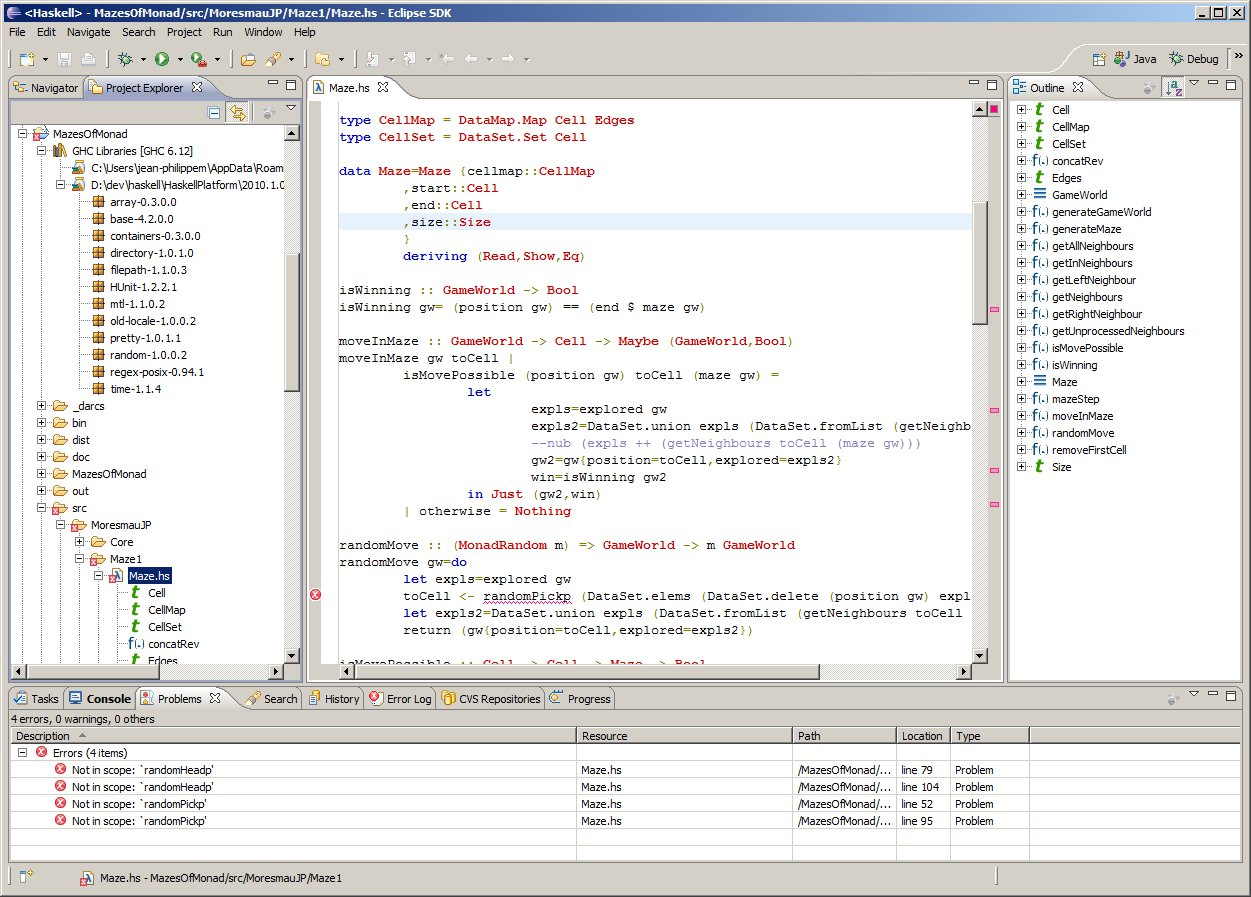
\includegraphics[scale=0.26]{Haskell1.jpg}
% 	\caption{Some Haskell code in a compiler.}
% \end{figure}

% This template has been designed for use in modern systems, but can perhaps be adapted to work on older systems, such as Windows 95. Below is a screenshot of a DOSBox console, an MS-DOS emulator designed to work on several platforms. Windows 95 can be installed into DOSBox, but it is not suggested.

% \begin{figure}[ht!]
% \centering
% 	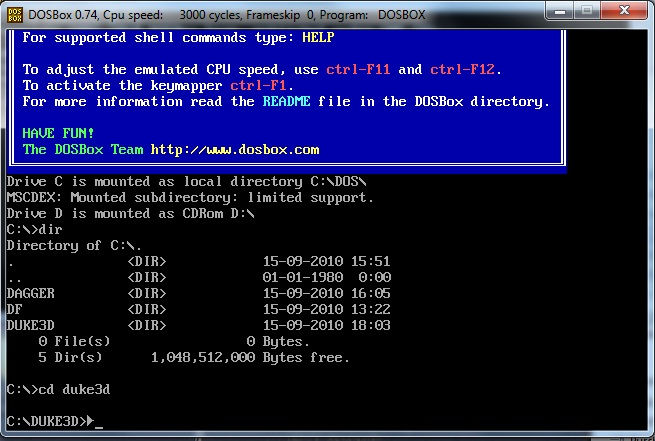
\includegraphics[scale=0.55]{DOSBox1.jpg}
% 	\caption{The DOSBox console running in Windows 7. The contents of the mounted directory C: are displayed, with the active subdirectory DUKE3D.}
% \end{figure}

% \section{Specifications in This TAMU \LaTeX ~ Template}

% All requirements for theses can be found in the most recent version of the Thesis Manual, available at the OGAPS website. The Thesis Office will be happy to assist you if you have questions about formatting. Questions specific to \LaTeX\ should be directed to \texttt{ogaps-latex@tamu.edu}.

% A common question students ask is the placement of a copyright statement at the beginning of a section with reprinted material from a previously printed source. The screenshot below describes how to achieve this. Check the instruction files for more details.

% \begin{figure}[ht!]
% \centering
% 	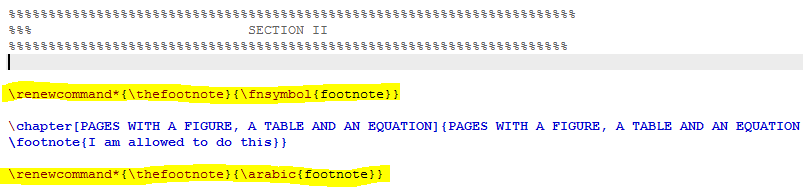
\includegraphics[scale=0.65]{Footnote.png}
% 	\caption{The inclusion of a copyright statement as a footnote. The lines in yellow help to change to footnote marking scheme.}
% \end{figure}

% \subsection{Another Test Section}
% There should be things here.

% %\begin{algorithm}
% %Stuff.
% %\end{algorithm}

% \subsubsection{Test}
% Hello, is it me you're looking for?

% \subsubsection{Test 2}
% There are more things to do.

% \subsection{Yet Another One}
% She called me late last night to say she loved me so. We insert a slew of figures in the remainder of the document to test the look of the List of Figures.

% \begin{figure}[H]
% 	\centering
% 	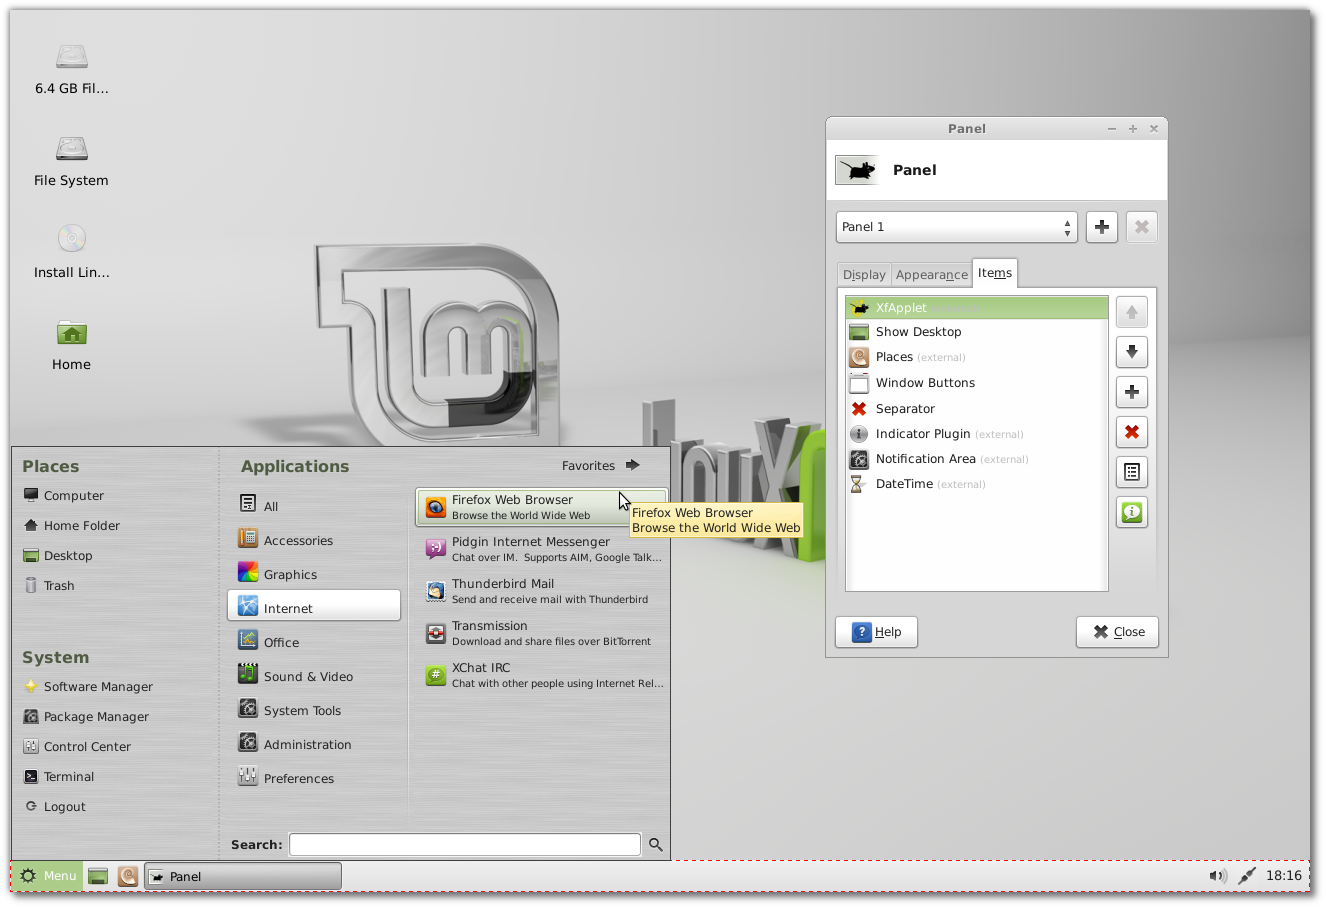
\includegraphics[width=4.25in]{Mint_XFCE.png}
% 	\caption{Linux Mint 13 with the XFCE desktop environment.}
% \end{figure}

% Another figure follows below.

% \begin{figure}[H]
% 	\centering
% 	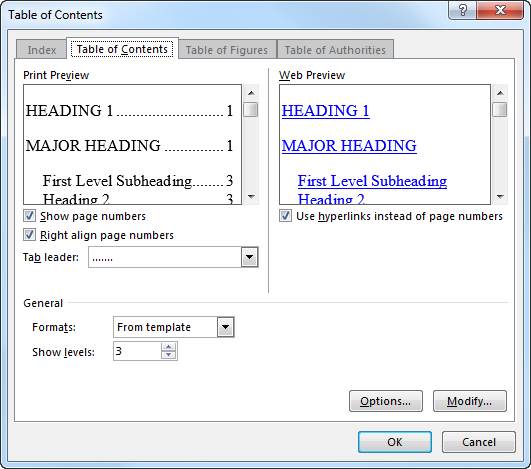
\includegraphics[scale=0.45]{TOC2.png}
% 	\singlespace
% 	\caption{The ``Table of Contents" dialog box in Microsoft Word. This must be accessed to properly generate the Table of Contents when using the Recommended Template.}
% \end{figure}

% Yet another figure follows - the last for this section.

% \begin{figure}[H]
% 	\centering
% 	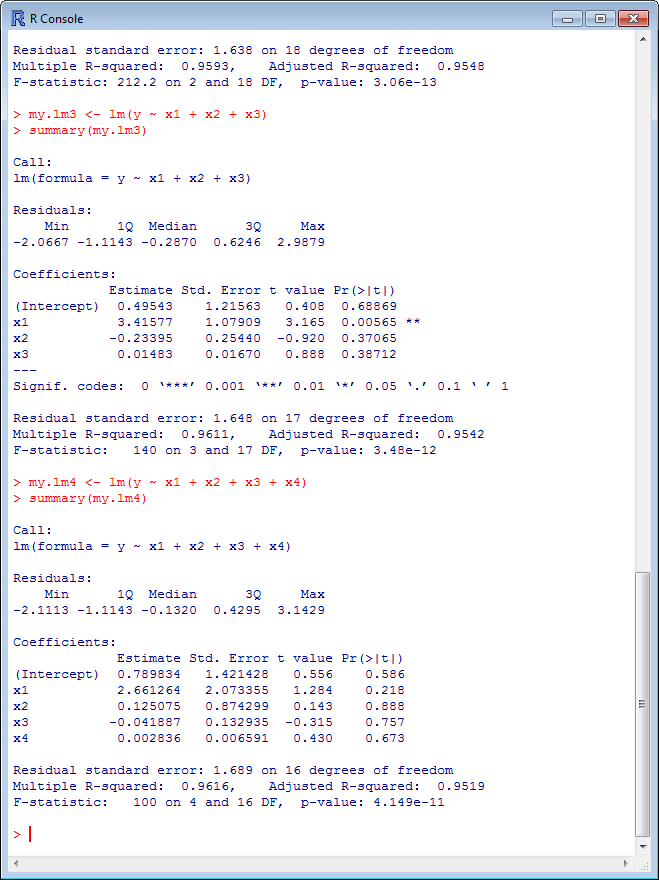
\includegraphics[width=3.75in]{Rachl3.png}
% 	\singlespace
% 	\caption{Linear regression on three (top) and four (bottom) independent variables in base R.}
% \end{figure}
 
%  \subsection{No Surprises Here}
%  Insert another song lyric here.


%%%%%%%%%%%%%%%%%%%%%%%%%%%%%%%%%%%%%%%%%%%%%%%%%%%
%
%  New template code for TAMU Theses and Dissertations starting Fall 2016.  
%
%
%  Author: Sean Zachary Roberson
%  Version 3.17.09
%  Last Updated: 9/21/2017
%
%%%%%%%%%%%%%%%%%%%%%%%%%%%%%%%%%%%%%%%%%%%%%%%%%%%

%%%%%%%%%%%%%%%%%%%%%%%%%%%%%%%%%%%%%%%%%%%%%%%%%%%%%%%%%%%%%%%%%%%%%%%
%%%                           SECTION II
%%%%%%%%%%%%%%%%%%%%%%%%%%%%%%%%%%%%%%%%%%%%%%%%%%%%%%%%%%%%%%%%%%%%%%


\chapter{THEORETICAL FRAMEWORK}
\section{The Standard Model}
Particle physics is the study of the fundamental constituents of matter and the forces between them. For more than 40 years these have been described by the so-called standard model of particle physics (SM), which provides, at least in principle, a basis for understanding most particle interactions, with the only exception of gravity.

The SM can be understood as a gauge theory combining the theory of electroweak interactions(EW) and quantum chromodynamics(QCD), or $SU(3)\times SU(2) \times U(1)$. 

\section{Structure and Particle Content}
In this section, the particle content of the SM will be intriduced, along with the various force carriers. In the following section, the specifics of particle-particle interactions will be explained in detail.

Elementary particles have an associated quantum number call spin, which allows for particle classification in terms of this quantity as fermions and bosons.

\subsection{Fermions}
Fermions are elementary particles with half-integer spin. They constitute the matter content of the SM, which accounts for 12 named fermions, which interact via the weak and electromagnetic force (with the exception of neutrinos). Also, they obey Fermi-Dirac statistics and the Pauli exclusion principle, meaning that no two fermions may be described by the same quantum numbers. Each fermion has its own anti-particle with the same mass but opposite quantum numbers.

The particle content of the SM can be divided into two additional categories of six fermions each, i.e. quarks and gluons. the quarks, which must bind together due to their strong force interaction and the leptons, which can exist independently. Quarks are known to bind into triplets and doublets, called baryons and mesons, respectively. Leptons come into three flavors, each one corresponding to a doublet where the electron, muon and tau are paired with a neutrino. %with the same quantum numbers?

Moreover, fermions are grouped into 3 families or generations of 4 particles (2 quarks and 2 leptons), according to their masses. Each subsequent generation being a heavier version of the previous generation, with the same quantum numbers (neutrinos may have a different mass order). Therefore, the particle formed from Generation I particles are usually more stable and long-lived than those made from Generation III particles. Protons and neutrins themselves are made up of up and down quarks.

%\subsubsection{Quarks}
%Quarks must bind together due to their strong force interaction. They are known to bind into triplets and doublets, called baryons and mesons, respectively.

%\subsubsection{Leptons}
%Leptons, unlike quarks, can exist independently. They come into three flavors, each one corresponding to a doublet where the electron, muon and tau are paired with a neutrino. %with the same quantum numbers?

\subsection{Bosons}
The SM bosons are the mediators of the interaction between the matter content of the SM, but also within themselves. They have integral spin quantum number and follow Bose-Einstein statistics. There are 5 named bosons, the gluons, photons, and W and Z with spin 1 since they go with vector fields, and the Higgs boson which corresponds to a scalar field and therefore has spin 0.

\section{Particle Interactions}
The interactions of the particles described in the previous section can be described in the mathematical framework of gauge field theory. Three of the four fundamental forces of nature are described in the SM (electromagnetism, the strong and the weak force). To each of these forces belongs a physical theory, its corresponding charge, (i.e. electric charge, color or flavor) and an associated boson as mediator.

Modern theories describe these forces in terms of Quantum fields, namely QED, QCD and the unified electroweak quantum field theory. One feature all these theories have in commmon is that they are all gauge invariant. This is important because this is a fundamental requirement from which the detailed properties of the interaction are deduced.

To describe each of the three SM interactions or forces, we will start with a Lagrangian that describes the dynamics of a given system of particles. Then we will take a look at the invariance of the Lagrangian after performing a local gauge transformation that will then require the introduction of gauge fields and their corresponding covariant derivatives. Finally, we will take a look at the conservation laws arising from the symmetry of the gauge invariance.

\subsection{Quantum Electrodynamics}

Quantum Electrodynamics (QED) describes the dynamics of the electromagnetic interaction between fermions and the boson mediating the interaction, the photon. QED corresponds to the $U_{EM}$ group and it was the first discovered example of gauge symmetry.% and it was developed from classical field theory.

In QFT, particles are represented by fields, which are in turn represented mathematically by Lagrangian densities $\mathcal{L}$. QED is described by the Dirac Lagrangian density
%If we start with the Lagrangian density for a free electron of mass m:

\begin{equation}
\mathcal{L} = \bar{\psi}(i\gamma^{\mu}\partial_{\mu} - m)\psi
\end{equation}

where $\gamma^{\mu}$ are the gamma matrices, $\phi$ is a four-component column vector representing the wave function of a spin 1/2 particle (or Dirac spinor), $\bar{\psi}=\psi^{\dagger}\gamma^{0}$, and $m$ is the mass of the particle. The Lagrangian is invariant under a global U(1) transformation

\begin{equation}
\psi \rightarrow \psi '= e^{-i\alpha}\psi
\end{equation}

while the parameter $\alpha$ is kept a constant. If instead, $\alpha$ is allowed to vary as a function of space-time, then equation (transformation) becomes a local U(1) transformation and the Lagrangian density becomes

\begin{equation}
\mathcal{L}\rightarrow \mathcal{L'} = \mathcal{L} + \bar{\psi}\gamma^{\mu}(\partial_{\mu}\alpha(x))\psi
\end{equation}

which is not invariant under the local transformation as is.

In order to restore local gauge invariance, a gauge field $A_{\mu}$ representing the photon and the covariant derivative 

\begin{equation}
D_{\mu} = \partial_{\mu} + iq A_{\mu}
\end{equation} 

, where $q = -e$ (electric charge) are introduced. The new gauge field transforms as

\begin{equation}
A_{\mu}\rightarrow A'_{\mu} = A_{\mu} + \partial_{\mu}\chi(x)
\end{equation}

, where $\chi(x)$ is an arbitrary function of space-time. The covariant derivative has the same transformation properties as $\psi$ and is chosen to replace $\partial_{\mu}$.

After introducing these modifications, the Lagrangian takes the form:

\begin{equation}
\mathcal{L} = \bar{\psi}(i\gamma^{\mu}D_{\mu}-m)\psi - \frac{1}{4}F_{\mu\nu}F^{\mu\nu}
\end{equation}

where $F_{\mu\nu}= \partial_{\mu}A_{\nu} - \partial_{\nu}A_{\mu}$ is the electromagnetic field strength tensor. 

An interesting result is that the Lagrangian does not contain a mass term for the newly-introduced photon field (i.e. no term $~m^{2}A_{\mu}A^{\mu}$), which explains the infinite range of the electromagnetic interaction. 

The final form of the Lagrangian includes lepton-photon interactions, those in the form of $l^{+}l^{-}\gamma$ and a quatric term in the field strngth tensor which is the photon kinetic energy. It can also be generalized to include all leptons by taking the form

\begin{equation}
\mathcal{L} = \sum_{i}\bar{\psi_{i}}(i\gamma^{\mu}D_{\mu}-m_{i})\psi_{i} - \frac{1}{4}F_{\mu\nu}F^{\mu\nu}
\end{equation}

where $i=e,\mu,\tau,u,d,c,s,t,b$.

\subsection{Electroweak Interaction}

The electroweak interaction is based on a local $SU(2)_{L}\times U(1)_{Y}$ gauge symmetry where $L $and $Y$ are the generators of the symmetry. As a result, electromagnetic and weak interactions are unified into a single non-abelian gauge theory. Also, just like in Section, the requirement of local gauge invariance leads to the introduction of gauge fields and determined the interactions mediated by those fields.

In order to understand this unification, we will first work with a fermionic doublet representing an $SU(2)$ symmetry

\begin{equation}
\psi = \begin{pmatrix}
	\psi_{1}(x) \\
	\psi_{2}(x)
\end{pmatrix}, u_{R}, d_{R}
\end{equation}

which transforms under the three dimensional rotation

\begin{equation}
\psi\rightarrow exp<i\alpha^{i}\frac{\sigma_{i}}{2}>\psi
\end{equation}

which is the three dimensional version of eq. and $\sigma^{i}$ are the Pauli sigma matrices.

Just like in the previous section, we allow the parameter $\alpha$ to vary as a function of space-time and thus

\begin{equation}
\psi(x)\rightarrow V(x)\psi(x)
\end{equation}
, where $V(x)= exp(i\alpha^{i}(x)\frac{\sigma^{i}}{2})$.

In order to keep the Lagrangian invariant under this transformation, we introduce three vector fields $A_{\mu}^{i}(x)$ and the covariant derivative

\begin{equation}
D_{\mu} = \partial_{\mu} - igA_{\mu}^{i}\frac{\sigma^{i}}{2}
\end{equation}

and therefore

\begin{equation}
A_{\mu}^{i}(x)\frac{\sigma^{i}}{2}\rightarrow V(x)(A_{\mu}^{i}(x)\frac{\sigma^{i}}{2}+\frac{i}{g}\partial_{\mu})V^{\dagger}(x)
\end{equation}

To simplify this calculation, we can expand $V(x)$ to first order in $\alpha$ 

\begin{equation}
A_{\mu}^{i}\frac{\sigma^{i}}{2}\rightarrow A_{\mu}^{i}\frac{\sigma^{i}}{2} + \frac{1}{g}(\partial_{\mu}\alpha^{i})\frac{\sigma^{i}}{2} + i[\alpha^{i}\frac{\sigma^{i}}{2}, A_{\mu}^{i}\frac{\sigma^{i}}{2}] + ...
\end{equation}

The covariant derivative will have the form

\begin{equation}
D_{\mu}\psi\rightarrow(1+i\alpha^{i}\frac{\sigma^{i}}{2})D_{\mu}\psi
\end{equation}

and the field strength tensor will be

\begin{equation}
F_{\mu\nu}^{i} = \partial_{\mu}A_{\nu}^{i} - \partial_{\nu}A_{\mu}^{i} + g\epsilon^{ijk}A_{\mu}^{j}A_{\nu}^{k}
\end{equation}
and the Yang-Mills Lagrangian becomes

\begin{equation}
\mathcal{L} = -\frac{1}{4}(F_{\mu\nu}^{i})^{2}+\bar{\psi}(i\gamma^{\mu}\partial_{\mu}-igA_{\mu}^{i}\frac{\sigma^{i}}{2})\psi
\end{equation}

Now we can obtain the interaction by following the same procedure as in the previous section, i.e., requiring local gauge invariance in the Lagrangian and introducing new gauge fields and covariant derivatives.

First we should note that the SM fermions possess a fundamental property called chirality, which describes how a given particle's wave function behaves under rotation. In the SM, the left-handed components of the electron neutrino and electron are grouped into an SU(2) doublet. Since the right-handed component of the electron is invariant under SU(2), it is placed in a singlet, i.e.:

\begin{equation}
L_{e} = \begin{pmatrix}
	\nu_{e} \\
	e_{L}
\end{pmatrix}
, e_{R}
\end{equation}
 And so on for the heavier generations of leptons. So far, there is no evidence of right-handed neutrinos in the SM.

 The kinetic energy term of the electroweak Lagrangian for first generation leptons can be represented by:

 \begin{equation}
 \mathcal{L}_{KE}^{e} = L_{e}^{\dagger}\tilde{\sigma}^{\mu}i\partial_{\mu}L_{e}+ e_{R}^{\dagger}\sigma^{\mu}i\partial_{\mu}e_{R}
 \end{equation}
where $\sigma = (\sigma^{0}, \sigma^{1},\sigma^{2}, \sigma^{3})$, $\tilde{\sigma} = (\sigma^{0}, -\sigma^{1},-\sigma^{2}, -\sigma^{3})$, $\sigma^{0}$ is an identity matrix, and the $\sigma^{i}$ are the Pauli matrices. This Lagrangian is invariant under the global $SU(2)_{L}\times U(1)_{Y}$ transformation:

\begin{equation}
L\rightarrow L' = e^{i\theta}UL\\
\end{equation}

\begin{equation}
e_{R}\rightarrow e'_{R} = e^{2i\theta}e_{R}
\end{equation}

where

\begin{equation}
U = e^{-ia^{k}\sigma^{k}}
\end{equation}

and $\theta$ and $a^{k}$ are real numbers parameterizing the transformation.
 However, the Lagrangian is not invariant under a transformation where these parameters are allowed to vary as a function of space-time, i.e. a local transformation.

Following the same reasoning as in the previous section, we can introduce gauge fields and replace the space-time derivatives with an appropiately chosen covariant derivative. This time, we introduce a U(1) gauge field $B_{\mu}(x)$ and three SU(2) gauge fields $W_{\mu}(x)= W_{\mu}^{k}(x)\sigma_{k}$. Such fields must transform as

\begin{equation}
B_{\mu}(x)\rightarrow B'_{\mu}(x) = B_{\mu}(x) + \frac{2}{g_{1}}\partial_{\mu}\theta(x)
\end{equation}
\begin{equation}
W_{\mu}(x)\rightarrow W'_{\mu}(x) = U(x)W_{\mu}(x)U^{\dagger}(x) + \frac{2i}{g_{2}}(\partial_{\mu}U(x))U^{\dagger}(x)
\end{equation}

where $g_{1}$ and $g_{2}$ are dimensionless parameters of the theory, the coupling strengths of the interactions. The necessary covariant derivatives are given by

\begin{equation}
D_{\mu}L_{e} = (\partial_{\mu}+i\frac{g_{1}}{2}YB_{\mu}+i\frac{g_{2}}{2}W_{\mu})L_{e}
\end{equation}

\begin{equation}
D_{\mu}e_{R} = (\partial_{\mu}+i\frac{g_{1}}{2}YB_{\mu})e_{R}
\end{equation}
 
 where Y is the hypercharge operator, whose eigenvalues are listed in Table 2.1. The weak hypercharge can be calculated as $Y=2(Q-T_{3})$, where $T_{3}$ is the third component of the weak isospin quantum number $T$.

 \begin{table}[h!]
	\centering
	\label{qun}
	\begin{tabular}{|l|l|l|l|l|l|l|}
		%\centering
		\hline
		                & Particle & Q   & $T_{3}$ & Y & B & L \\ \hline
		Quarks          & $q_{L} = \begin{pmatrix}
									u \\
									d
									\end{pmatrix}_{L}$ & $\begin{pmatrix} 2/3 \\ -1/3 \end{pmatrix}$  & $\begin{pmatrix} 1/2 \\ -1/2 \end{pmatrix}$ & 1/3 & 1/3 & 0 \\ 
		                & $u_{R}$ & 2/3 & 0 & 4/3 & 1/3 & 0 \\ 
		                & $d_{R}$ & -1/3& 0 & -2/3 & 1/3 & 0 \\ \hline
		Leptons         & $l_{L} = \begin{pmatrix} \nu_{e}\\ e \end{pmatrix}_{L}$ & $\begin{pmatrix} 0 \\ -1 \end{pmatrix}$ & $\begin{pmatrix} 1/2 \\ -1/2 \end{pmatrix}$ & -1 & 0 & 1 \\
		                & $e_{R}$ & -1 & 0 & -2 & 0 & 1 \\ \hline
	
	\end{tabular}
	\caption{Quantum numbers of the SM fermions}
\end{table}

 These covariant derivatives transform according to the same rule as the fields themselves. Combining the kinetic and gage interaction terms of the Lagrangian yields

 \begin{equation}
 \mathcal{L} = \mathcal{L}_{KE} + \mathcal{L}_{gauge}= L_{e}^{\dagger}\tilde{\sigma}^{\mu}iD_{\mu}L_{e}+e_{R}^{\dagger}\sigma^{\mu}iD_{\mu}e_{R} - \frac{1}{4}B_{\mu\nu}B^{\mu\nu}- \sum_{i=1}^{3}\frac{1}{4}W_{\mu\nu}^{i}W^{i\mu\nu}
 \end{equation}

 where $B_{\mu\nu}=\partial_{\mu}B_{\nu}-\partial_{\nu}B_{\mu}$ and $W_{\mu\nu} = [\partial_{\mu}+(\frac{ig_{2}}{2})W_{\mu}]W_{\nu} - [\partial_{\nu}+(\frac{ig_{2}}{2})W_{\nu}]W_{\mu}$ are the field strength tensors. This Lagrangian is now locally invariant.

 The mediators of the electroweak force are the physical bosons $W^{\pm}$, the Z and the photon. All these are combinations of the gauge fields in the following way. 

 The $W^{\pm}$ are linear combinations of the $W_{1}$ and $W_{2}$, which are electrically charged and given by

 \begin{equation}
W_{\mu}^{\pm} = \frac{W_{\mu}^{1}\mp i W_{\mu}^{2}}{\sqrt{2}}
 \end{equation}

The $W_{3}$ and $B$ gauge fields are electrically neutral. The physical Z and photon are linear combinations of these fields, given by

\begin{equation}
Z_{\mu} = W_{\mu}^{3}cos\theta_{W} - B_{\mu}sin\theta_{W}
\end{equation}
\begin{equation}
A_{\mu} = W_{\mu}^{3}sin\theta_{W} - B_{\mu}cos\theta_{W}
\end{equation}

where the Weinberg angle $\theta_{W}$ is defined by $sin\theta_{W}= g_{1}/\sqrt{g_{1}^{2}+g_{2}^{2}}$.

Now, the interactions contained in the Lagrangian only couple the $W^{\pm}$ to the left-handed lepton components, but couple the Z and photon to both the left- and right-handed components. 

We can also see from here that the interaction strength is equal to the electromagnetic charge unit $e$, i.e. $g_{2}sin\theta_{W}=g_{1}cos\theta_{W}=e$.

Finally, in order to include second and third generation leptons, the Lagrangian generalizes to 

\begin{equation}
\mathcal{L}^{l} = \sum_{leptons}(L_{e}^{\dagger}\tilde{\sigma}^{\mu}iD_{\mu}L_{e}+e_{R}^{\dagger}\sigma^{\mu}iD_{\mu}e_{R}) - \frac{1}{4}B_{\mu\nu}B^{\mu\nu}- \sigma_{i=1}^{3}\frac{1}{4}W_{\mu\nu}^{i}W^{i\mu\nu}
\end{equation}

Quarks are included in the electroweak sector in a similar manner. The left-handed components of the $u$ and $d$ quark are place in SU(2) doublets, and the right-handed components in singlets.

\begin{equation}
Q_{u} = \begin{pmatrix}
	u_{L} \\
	d_{L}
\end{pmatrix}, u_{R}, d_{R}
\end{equation}
Two additional doublets and four singlets exist for the second and third generation quarks. The covariant derivatives acting on the quark fields are the same as those which act on the lepton fields, but the quarks have different weak hypercharge assignments from the leptons. Therefore, the dynamic portion of the $u$ and $d$ quark Lagrangian is given by:

\begin{equation}
\mathcal{L}^{q}_{KE} = \sum_{quarks}Q_{u}^{\dagger}\tilde{\sigma}^{\mu}iD_{\mu}Q_{\mu}+u_{R}^{\dagger}\sigma^{\mu}iD_{\mu}u_{R}+d^{\dagger}_{R}\sigma^{\mu}iD_{\mu}d_{R}
\end{equation}
Again, the W bosons couple only to the left-handed quark components, while the Z and photon couple to the right-handed components as well.

The full electroweak Lagrangian is a result of the addition of the lepton and quark kinetic components, as well as the gauge interaction component.

\begin{equation}
\mathcal{L}^{EW} = \mathcal{L}^{l}_{KE} + \mathcal{L}_{KE}^{q} + \mathcal{L}_{gauge}
\end{equation}

Here, we should notice that a couple of symmetries arise from the form of the Lagrangian in Eq. If a U(1) transformation of the form $L_{e,\mu,\tau}\rightarrow e^{i\alpha}L_{e,\mu,\tau}$, $e,\mu,\tau_{R}\rightarrow e,\mu,\tau^{i\alpha}e,\mu,\tau_{R}$ leaves the Lagrangian invariant, which leads to conservation of lepton number. Additionally, a U(1) transformation multiplying all negatively (positively) charged fields by $e^{i\alpha}(e^{-i\alpha})$ leaves the Lagrangian invariant, and implies conservation of electric charge.

On the other hand, the EW Lagrangian is not invariant under charge conjugation $C$ of a parity conservation $P$. Charge conjugation is the operation of changing the sign of all discrete quantum numbers, or equivalently exchanging all particles with antiparticles and vice-versa. A parity transformation is the inversion of spatial coordinates, $r\rightarrow -r$. The neutral current interactions, mediated by the Z and photon, preserve combined CP invariance. However, even combined CP symmetry is violated by weak current interactions, mediated by the $W^{\pm}$, in the quark sector. A third important potential symmetry is time reversal $T$, where $t\rightarrow -t$. Combined CPT invariance is required to mantain Lorentz invariance. Therefore, the breaking of CP also implied the breaking of T symmetry.

Finally, a notable property of the weak interaction is that it only acts on particles with weak isospin quantum number T and that $T_{3}$ is conserved in all interactions.

\subsection{Strong Interaction}

	Quantum Chromodynamics is the theory that describes the interaction between quarks via the strong force. It is represented by a local $SU(3)_{C}$ gauge symmetry and the interaction mediator is the gluon.

	Its corresponding charge is the color. Color charges can be green, red, and blue but only color neutral (or colorless) hadrons are allowed in nature. Baryons contain equal parts of each color and mesons contain color-anticolor pairs.

	In QCD, quarks are represented in this theory as color triplets

	\begin{equation}
	q_{u} = 
	\begin{pmatrix}
		u_{r} \\
		u_{g}\\
		u_{b}
	\end{pmatrix}
	\end{equation}

	and gluons contain two color charges. The eight known combinations of color charges for the gluon are represented by eight gauge fields that will be introduced below.

	As in the previous sections, we start building the interaction from an $SU(3)$ Lagrangian that is globally invariant in the form

	\begin{equation}
	\mathcal{L}^{q}_{QCD} = \sum_{i=1}^{6}\bar{q}_{i}i\gamma^{\mu}\partial_{\mu}q_{i}
	\end{equation}

	This Lagrangian is invariant under a transformation of the form $q_{i}\rightarrow q_{i}' = Uq_{i}$ where $U$ is a member is a member of $SU(3)$. If we allow for a transformation of the for $U(x)$, the Lagrangian is no longer invariant. To return invariance, we introduce 8 gauge fields ($G_{\mu}(x)$), which represent the gluons and an appropiate covariant derivative.
	
	The transformation of the gauge fields and the covariant derivative will take the form:
		\begin{equation}
		G_{\mu}\rightarrow G'_{\mu} = UG_{\mu}U^{\dagger}+\frac{i}{g_{s}}(\partial_{\mu}U)U^{\dagger}
		\end{equation}
		\begin{equation}
		D_{\mu}q_{i} = (\partial_{\mu}+ig_{s}G_{\mu})q_{i}
		\end{equation}
		where $g_{s}$ is the dimensionless coupling strength of the color interaction.
	The field strength tensor for QCD is:
		\begin{equation}
		G_{\mu\nu} = \partial_{\mu}G_{\nu} - \partial_{v}G_{\mu} + ig_{s}(G_{\mu}G_{\nu} - G_{\nu}G_{\mu})
		\end{equation}
	and the locally $SU(3)$ gauge invariant QCD Lagrangian is then given as:
		\begin{equation}
		\mathcal{L}^{q}_{QCD} = \sum_{i=1}^{6}(\bar{q}_{i}i\gamma^{\mu}D_{\mu}q_{i})-\frac{1}{4}\sum_{i=1}^{8}G_{\mu\nu}^{i}G^{i\mu\nu}
		\end{equation}

	In contrast to the EW interaction, C,P, and T are all conserved. The Strong force interaction range is about $10^{-15}$ which is enough to act on nucleons, i.e. protons and neutrons to form atomic nuclei.
	
	QCD is a strongly coupled theory at low energies and large distance scales and weakly interacting at high energies and small distance scales. This fact is responsible for the hadronic bound states of quarks.
		%\item Asymptotic freedom, strong force between quarks increases as they move farther apart until energy is so large that nature prefers to create a new quark-antiquark pair.
	At low energy scales, i.e. non-perturbative regime, QCD calculations are extremely difficult and techniques as lattice gauge theory must be exploited.
	On the other hand, at a high energy scale, or equivalently small distance scales, the strong interaction becomes weakly interacting and quarks are effectively free. In this regime the usual techniques of perturbation theory can be used, allowing high-precision calculations.

\subsection{Brout-Englert-Higgs Mechanism and the Higgs Boson}
	As we have seen from the previous section, the EW and QCD Lagrangians do not contain any mass terms. This implies that the SM bosons should be massless, which contradicts the experimental results since the $W^{\pm}$ and Z bosons do indeed have mass. This is a result of the requirement of local $SU(3)_{C}\times SU(2)_{L}\times U(1)_{Y}$ gauge invariance in the Lagrangian.

	The Brout-Englert-Higgs mechanism allows for W and Z bosons to have mass while preserving gauge invariance by adding one or more complex scalar fields, the Higgs field(s) to the SM Lagrangian. These fields will acquire a vacuum expectation value which will spontaneously break the symmetry of the Lagrangian. 

	The Goldstone theorem tells us that for every spontaneously broken continuous symmetry there will be a new massive scalar "Goldstone" boson. The number of new bosons will be equal to the number of broken generators of the symmetry group. The massless SM bosons then acquire mas by absorbing these Goldstone bosons.
	
	THe BEH mechanism is also used to generate mass for the quarks and electrically charged leptons. The neutrinos, photon, and gluons remain massless, as observed experimentally.
	
	Remember from previous section that there are four massless electroweak gauge bosons, $W^{1}, W^{2}, W^{3}$, and $B^{0}$. The experimentally observed bosons, however, are the massless photon, and three massive bosons (the $W^{\pm}$ and Z). We also know that electric charge Q is conserved in electroweak interactions. This means that the $SU(2)_{L}\times U(1)_{Y}$ electroweak theory is broken such that a new $U(1)_{EM}$ symmetry group is formed which corresponds to electromagnetism. 
	
	In order for three gauge bosons to acquire mass they must absorb three Goldstone bosons. The simplest method to acomplish this is to introduce a complex, scalar $SU(2)$ doublet $\Phi$ with hypercharge $Y=1$.
	\begin{equation}
		\Phi = \begin{pmatrix}
		\Phi_{A} \\
		\Phi_{B}
		\end{pmatrix} = \begin{pmatrix} \phi_{1} \\ i\phi_{2} \\ \phi_{3} \\ i\phi_{4} \end{pmatrix},
	\end{equation}

	The part of the SM Lagrangian which includes the electroweak gauge bosons and the leptons can be written as

	\begin{equation}
	\mathcal{L}_{SM} = -\frac{1}{4}W_{\mu\nu}^{a}W_{a}^{\mu\nu} - \frac{1}{4}B_{\mu\nu}B^{\mu\nu} + \bar{L}_{i}(iD_{\mu}\gamma^{\mu})L_{i} + \bar{e}_{R,i}(iD_{\mu}\gamma^{\mu})e_{R,i}
	\end{equation}

	where $i$ runs over the three generations, $\mu$ and $\nu$ are Lorentz indices, and $a$ runs over the generators in the gauge group. The field strengths are given by

	\begin{equation}
	W_{\mu\nu}^{a} = \partial_{\mu}W_{\nu}^{a} - \partial_{\nu}W_{\mu}^{a} + g_{2}\epsilon^{abc}W_{\mu}^{b}W_{\nu}^{c}
	\end{equation}
	\begin{equation}
	B_{\mu\nu} = \partial_{\mu}B_{\nu} - \partial_{\nu}B_{\mu}
	\end{equation}

	and the covariant derivatives for the left- and right-handed leptons are

	\begin{equation}
	D_{\mu}L_{L} = (\partial_{\mu}- ig_{2}T_{a}W_{\mu}^{a}-ig_{1}YB_{\mu})L_{L}
	\end{equation}
	\begin{equation}
	D_{\mu}e_{R} = (\partial_{\mu}- ig_{1}YB_{\mu})e_{R}
	\end{equation}

	where $T_{a}$ are the generators of the $SU(2)_{L}$ gauge group and $g_{1},g_{2}$ are the coupling constants for the electroweak interaction.

	The scalar part of the Lagrangian required by the addition of a scalar field is then
		\begin{equation}
			\mathcal{L}_{S} = (D_{\mu}\Phi)^{\dagger}(D^{\mu}\Phi) - V(\Phi^{\dagger}\Phi)
		\end{equation}

	where the first term is the kinetic term and the second term is the scalar potential. While the form of the scalar potential is not known from first principles, we can make the assumption that it takes the simplest form possible which has the desired properties of spontaneous symmetry breaking and the ability to be renormalized. Then

		\begin{equation}
		V(\Phi^{\dagger}\Phi) = \mu^{2}\Phi^{\dagger}\Phi+\lambda(\Phi^{\dagger}\Phi)^{2}
		\end{equation}

	The value of $\lambda$ must be positive in order for the vacuum to be stable. The sign of $\mu^{2}$ specifies one of two cases for the potential.

	\begin{itemize}
			\item When $\mu^{2}>0$, the potential $V(\Phi)$ is always positive and has a minimum at

			\begin{equation}
			<0|\Phi|0>\equiv\Phi_{0} = \begin{pmatrix} 0 \\ 0 \end{pmatrix}
			\end{equation}

			where no spontaneous symmetry breaking can occur. 

			\item When $\mu^{2}<0$ the potential has a minimum value not located at the origin. In this case, the neutral component of the scalar field will acquire a vacuum expectation value $v$, a process that we will refer to as electroweak symmetry breaking (EWSB).

			\begin{equation}
			<0|\Phi|0> = \Phi_{0} = \frac{1}{\sqrt{2}}\begin{pmatrix} 0 \\ v \end{pmatrix}
			\end{equation}

			where $v=\sqrt{\frac{-\mu^{2}}{\lambda}}$
	\end{itemize}

	
	By only adding a $vev$ to the neutral component of the scalar field, electromagnetism is unbroken and the $U(1)_{EM}$ symmetry keeps a conserved electric charge $Q=T_{3}+\frac{Y}{2}$.

	We can then expand the scalar field $\Phi$ around the minimum $\Phi_{0}$ to get 

		\begin{equation}
			\Phi(x) = \frac{1}{\sqrt{2}}\begin{pmatrix} 0 \\ v + h(x) \end{pmatrix}
		\end{equation}

	where $h(x)$ is a new scalar field.

	Next we insert this field into the kinetic part of the Lagrangian and redefine the gauge fields as 

		\begin{equation}
		W_{\mu}^{\pm} = \frac{1}{\sqrt{2}}(W_{\mu}^{1}\mp iW_{\mu}^{2})
		\end{equation}

		\begin{equation}
		Z_{\mu} = \frac{1}{\sqrt{g_{1}^{2}+g_{2}^{2}}}(g_{2}W_{\mu}^{3}-g_{1}B_{\mu})
		\end{equation}

		\begin{equation}
		A_{\mu} = \frac{1}{\sqrt{g_{1}^{2}+g_{2}^{2}}}(g_{2}W_{\mu}^{3}+g_{1}B_{\mu})
		\end{equation}

		which correspond to the observed gauge bosons. 

	After this the covariant derivative becomes

		\begin{equation}
		|D_{\mu}\Phi|^{2} = \frac{1}{2}(\partial_{\mu}H)^{2}+\frac{1}{2}g_{2}^{2}(v+H)^{2}W_{\mu}^{+}W^{\mu-}+\frac{1}{8}(v+H)^{2}(g_{1}^{2}+g_{2}^{2})Z_{\mu}Z^{\mu}
		\end{equation}

	From here we can see that the photon $A_{\mu}$ remains massless, but that the mass terms for the $W$ and $Z$ bosons take the general forms $M_{W}^{2}W_{\mu}W^{\mu}$ and $M_{Z}^{2}Z_{\mu}Z^{\mu}/2$ respectively.

	Thus the masses of the electroweak gauge bosons are

		\begin{equation}
		M_{W} = \frac{1}{2}vg_{2}
		\end{equation}
		\begin{equation}
		M_{Z}= \frac{1}{2}v\sqrt{g_{1}^{2}+g_{2}^{2}}
		\end{equation}
		\begin{equation}
		M_{A} = 0
		\end{equation}

	Three of the degrees of freedom from the scalar field, which would have been two charged and one neutral Goldstone boson, have been absorbed by the gauge bosons in order to give them mass. There is one remaining degree of freedom, an oscillation in the radial direction of the scalar potential, which corresponds to the neutral Higgs boson.

	Finally, fermions acquire mass by adding couplings between the fermion fields and the scalar field to the SM Lagrangian. The part of the Lagrangian that corresponds to the first generation fermions is given by

		\begin{equation}
		\mathcal{L}_{F} = -G_{e}\bar{L}\Phi e_{R} - G_{d}\bar{Q}\Phi d_{R} - G_{u}\bar{Q}\tilde{\Phi}u_{R}+h.c.
		\end{equation}

	where $\tilde{\Phi}=i\tau_{2}\Phi^{*}$ is the conjugate of $\Phi$ with negative hypercharge.

	There are additional terms added to the full Lagrangian which correspond to the second and third generations which are not shown here.

	By substituting $\Phi$ into the previous Lagrangian we find

		\begin{align}
		\mathcal{L}_{F} &= -\frac{1}{\sqrt{2}}[G_{e}\begin{pmatrix} \bar{\nu} & \bar{e} \end{pmatrix}_{L}\begin{pmatrix} 0 \\ v+H \end{pmatrix}e_{R}+G_{d}\begin{pmatrix}\bar{u} & \bar{d}\end{pmatrix}_{L}\begin{pmatrix} 0 \\ v+H \end{pmatrix}d_{R} + G_{u}\begin{pmatrix}\bar{u} & \bar{d}\end{pmatrix}_{L}\begin{pmatrix} 0 \\ v+H \end{pmatrix}u_{R}] + h.c. \\
		&= -\frac{1}{\sqrt{2}}(v+H)(G_{e}\bar{e}_{L}e_{R}+G_{d}\bar{d}_{L}d_{R}+G_{u}\bar{u}_{L}u_{R})+h.c. 
		\end{align}

	where $h.c.$ is a placeholder for the hermitian conjugate terms. 

	The fermion masses take the form $m\bar{f}_{L}f_{R} + h.c.$, which means that the fermion masses for the first generation are

		\begin{equation}
		m_{e} = \frac{G_{e}v}{\sqrt{2}}, m_{u}=\frac{G_{u}v}{\sqrt{2}}, m_{d}=\frac{G_{d}v}{\sqrt{2}} 
		\end{equation}

	The second and third generations have similar mass terms. For the case of the neutrinos, since there is no right handed neutrino in the SM the neutrinos that do exist remain massless.
	
	Finally, the coupling constants, $G$, and the fermion masses are not predicted by the SM, so they must be measured and added to the model.

\section{Beyond the Standard Model}
\begin{itemize}
The SM evolved in response to a series of experimental discoveries over a period of several decades, and it turned out to be a remarkably successful theory. At the present time, provided non-zero neutrino masses are incorporated, all experimental observations in particle physics are consistent with the SM, but there is no reason to suppose that there will not be more surprises in the future, as higher energy regions are explored.

Also, there are a few experimental hints which suggest that the SM may not be a complete theory of nature. For example, there is strong evidence that the particles of the SM can only account for a small fraction of the matter in the Universe, and the observed predominance of matter over antimatter cannot be understood in the framework of the SM.

Moreover, although evidence has recently been reported for the existence of gravitational waves, which are a necessary consequence of any quantum theory of gravity, we have no consistent theory of quantum gravity.

Finally, the SM itself embodies many assumptions and more than twenty free parameters, giving rise to many questions like

\begin{itemize}
 \item Can the number of prameters be reduced?
 \item Why are there three families of quarks and leptons, rather than just the one that is required to describe "ordinary matter", i.e. the neutrons and protons?
 \item Are the quarks really point-like particles, or will they turn out to be composite when we are able to explore a higher energy regime?
 \item Why does the weak interaction violate CP invariance, but not the strong interaction?
\end{itemize}

Many theories have been proposed to try to answer these and other questions, and a few experimental programmes have been set up to test them. %They typically predict the existence of particles or unknown phenomena beyond the SM.

\section{Lepton universality}
%One of the current assumptions of the SM is that electron, muon, and tau couplings are the same when interacting weakly. This is often referred to as lepton universality. 
	All known experimental data are consistent with the assumption that the interactions of the electron and its neutrino are identical with those of the muon and its associated neutrino and the tau and its neutrino, provided the mass differences are taken into account. This fundamental assumption is called the universality of lepton interactions.

	We will illustrate universality of this rule by looking at the leptonic decays \cite{MartinShaw}

	\begin{align}\label{eq2.4.1}
	\mu^{+}&\rightarrow e^{+} + \nu_{e} + \bar{\nu}_{\mu},\\
	\mu^{-}&\rightarrow e^{-} + \bar{\nu}_{e} + \nu_{\mu},\\
	\tau^{-}&\rightarrow \mu^{-} + \bar{\nu}_{\mu} + \nu_{\tau}, and\\
	\tau^{-}&\rightarrow e^{-} + \bar{\nu}_{e} + \nu_{\tau}
	\end{align}
	of the muon and tau leptons at rest. 

	To simplify the calculation, we will work to lowest order only and we will use the zero-range approximation (a zero-range point interaction with strength equal to the Fermi constant $G_{F}=1.66\times 10^{-5} GeV^{-2}$), since the masses of the leptons are very small ompared with the rest energy of the W bosons mediating the weak interaction.

	We start by considering the muon decay whose rate has the form (in the zero-range appproximation)

	\begin{equation}\label{eq2.4.2}
	\Gamma(\mu^{-}&\rightarrow e^{-} + \bar{\nu}_{e} + \nu_{\mu}) = KG_{F}^{2}m_{\mu}^{5}
	\end{equation}

	since we are assuming the electron and neutrino masses are zero. Here, $K$ is a dimensionless constant whose value will depend on the precise form of the interaction. If we assume this is the same for muon and tau leptons the same argument gives

	\begin{equation}
	\Gamma(\tau^{-}&\rightarrow e^{-} + \bar{\nu}_{e} + \nu_{\tau}) = KG_{F}^{2}m_{\tau}^{5}
	\end{equation}

	Likewise, $e - \mu$ universality gives

	\begin{equation}
	\Gamma(\tau^{-}&\rightarrow e^{-} + \bar{\nu}_{e} + \nu_{\tau}) = \Gamma(\tau^{-}&\rightarrow \mu^{-} + \bar{\nu}_{\mu} + \nu_{\tau})
	\end{equation}

	This explains why the experimental branching ratios for the two leptonic decay modes of the tau lepton are, to a good approximation, equal. A full calculation, taking into account final state masses, gives the ratio $\Gamma(\tau^{-}&\rightarrow \mu^{-} + \bar{\nu}_{\mu} + \nu_{\tau})/\Gamma(\tau^{-}&\rightarrow e^{-} + \bar{\nu}_{e} + \nu_{\tau})=0.973$, whereas the experimental value is $0.976\pm0.003$.

	It also gives a relation between the $\mu$ and $\tau$ lifetimes 

	\begin{equation}
	\tau_{l}= \frac{1}{\Gamma_{tot}} = \frac{B(l^{-}\rightarrow e^{-}\bar{\nu}_{e}\nu_{l})}{\Gamma(l^{-}\rightarrow e^{-}\bar{\nu}_{e}\nu_{l})}
	\end{equation}

	where $l$ can be the $\mu$ or $\tau$ lepton and $\Gamma_{tot}$ is the total decay rate and therefore

	\begin{equation}
	B(l^{-}\rightarrow e^{-}\bar{\nu}_{e}\nu_{l}) = \frac{\Gamma(l^{-}\rightarrow e^{-}\bar{\nu}_{e}\nu_{l})}{\Gamma_{tot}}
	\end{equation}

	is the branching ratio. Experimentally, $B=1$ and $0.1783\pm0.0004$ for $l=\mu$ and $\tau$. Thus from \ref{eq2.4.1}and \ref{eq2.4.2} we have

	\begin{equation}
	\frac{\tau_{\tau}}{\tau_{\mu}} = \frac{B(\tau^{-}\rightarrow e^{-}\bar{\nu}_{e}\nu_{\tau})}{B(\mu^{-}\rightarrow e^{-}\bar{\nu}_{e}\nu_{\mu})}\(\frac{m_{\nu}}{m_{\tau}}\)^{5} = (1.326\pm0.003)\times 10^{-7}
	\end{equation}

	This agreement, involving lifetimes that differ by seven orders of magnitude, is impressive evidence of the universality of lepton interactions.

\section{B-hadron anomalies}
	So far, no definite violation of this rule has been observed, but recent studies involving the decay rates of B mesons seem to challenge it. BaBar, LHCb and Belle experiments have reported anomalous deviations from SM in measurements of:

	\begin{enumerate}
    	\item The angular distributions of the decay rate of $B\rightarrow K^{*}\mu^{+}\mu^{-}$.
    	\item The branching ratios $R_{K} = \frac{BR(B^{+}\rightarrow K^{+}\mu^{+}\mu^{-})}{BR(B^{+}\rightarrow K^{+}e^{+}e^{-})}$ and $R_{K^{*}} = \frac{BR(B^{+}\rightarrow K^{*}\mu^{+}\mu^{-})}{BR(B^{+}\rightarrow K^{*}e^{+}e^{-})}$.
	\end{enumerate}
Each of these results show a deviation from the expected SM value of 1 in the 2.4-2.6 $\sigma$ range. These decay processes are very rare in the SM, making it hard to obtain a precise measurement. Also, a better understanding of the SM physics behind them (in terms of hadronic uncertainties) could also provide reconciliation with SM predictions. A more recent study combined the results for $R_{K}$ and $R_{K^{*}}$, resulting in a 4$\sigma$ deviation from the SM. 

\subsection{$b\rightarrow s$ quark transitions}
This anomaly hints at the posibility that $b\rightarrow s$ quark transitions cannot be understood entirely within the SM framework. 

Within the SM, the lowest order processes that could mediate the $b\rightarrow s$ quark transitions are at least of third order. Therefore, these processes are rarely observed.

\section{The Z'}
As an alternative, a possible explanation to the B-decay anomalies could postulate the existence of a new heavy neutral gauge boson, the Z'. Such a particle would couple to $b-s$ quarks and non-universally to leptons. In addition, it would be assumed to couple mostly to third generation quarks to explain why it has not been seen yet by any experiment.
%Basic properties/ Feynman diagram
\subsection{Flavour-violating coupling $\delta_{bs}$}
In order to provide an explanation for B-decay anomalies, we need to consider the flavour-violating coupling $\delta_{bs}$. Allowing the Z' boson to couple to $s$ quarks in addition to $b$ quarks results in two times more ways to produce the Z' and two times more ways for it to decay. A non-zero $\delta_{bs}$ will allow the Z's to be produced by $b$ and $\bar{s}$ quarks (in addition to $b\bar{b}$ ones) and this significantly enhances the production cross section.

\subsection{Lifetime calculation}
\subsection{4b Bottom Fermion Fusion}
If we make the assumption that the Z' couples mostly to b quarks, the particle could have diagrams like the on on Figure, which we will refer to as Bottom Fermion fusion diagram (BFF) due to its similarity with Vector Boson Fusion (VBF) diagrams.
%%%%%%%%%%%%%%%%%%%%%%%%%%%%%%%%%%%%%%%%%%%%%%%%%%%%
%
%  New template code for TAMU Theses and Dissertations starting Fall 2016.  
%
%
%  Author: Sean Zachary Roberson
%  Version 3.17.09
%  Last Updated: 9/21/2017
%
%%%%%%%%%%%%%%%%%%%%%%%%%%%%%%%%%%%%%%%%%%%%%%%%%%%
%%%%%%%%%%%%%%%%%%%%%%%%%%%%%%%%%%%%%%%%%%%%%%%%%%%%%%%%%%%%%%%%%%%%%%
%%                           SECTION III
%%%%%%%%%%%%%%%%%%%%%%%%%%%%%%%%%%%%%%%%%%%%%%%%%%%%%%%%%%%%%%%%%%%%%

\chapter{The LHC and CMS Detector}
\section{The Large Hadron Collider}

The Large Hadron Collider (LHC) \cite{Breskin:1244506} experiment at the European ORganization for Nuclear Research (CERN) is the world's largest and most powerful particle accelerator in operation today. Located at the border between Switzerland and France, it consists of a 27-km circumference ring of superconducting magnets and accelerating structures.

Within the ring, protons are accelerated to a speed close to that of light and made to collide at 4 points:

\begin{itemize}
\item CMS (Compact Muon Solenoid) \cite{Chatrchyan:2008aa},
\item ATLAS (A Toroidal LHC ApparatuS) \cite{1748-0221-3-08-S08003},
\item ALICE (A Large Ion Collider Experiment) \cite{Aamodt:2008zz},
\item and LHCb (Large Hadron Collider beauty) \cite{Alves:2008zz}.
\end{itemize}

ATLAS and CMS are the two general-purpose particle detectors located at opposite sides on the LHC ring. These are "onion-type" detectors in the sense that their general layout surrounds the interaction point with sub-detector systems aimed to measure a specific property of the particle to be detected.

The other two detectors, ALICE and LHCb are designed for specific purposes, like studying heavy-ion collisions and performing precision measurements of CP-violation and the physics of B-mesons, respectively. For this study we are going use data collected by the CMS experiment.

 \begin{figure}[H]
 	\centering
 	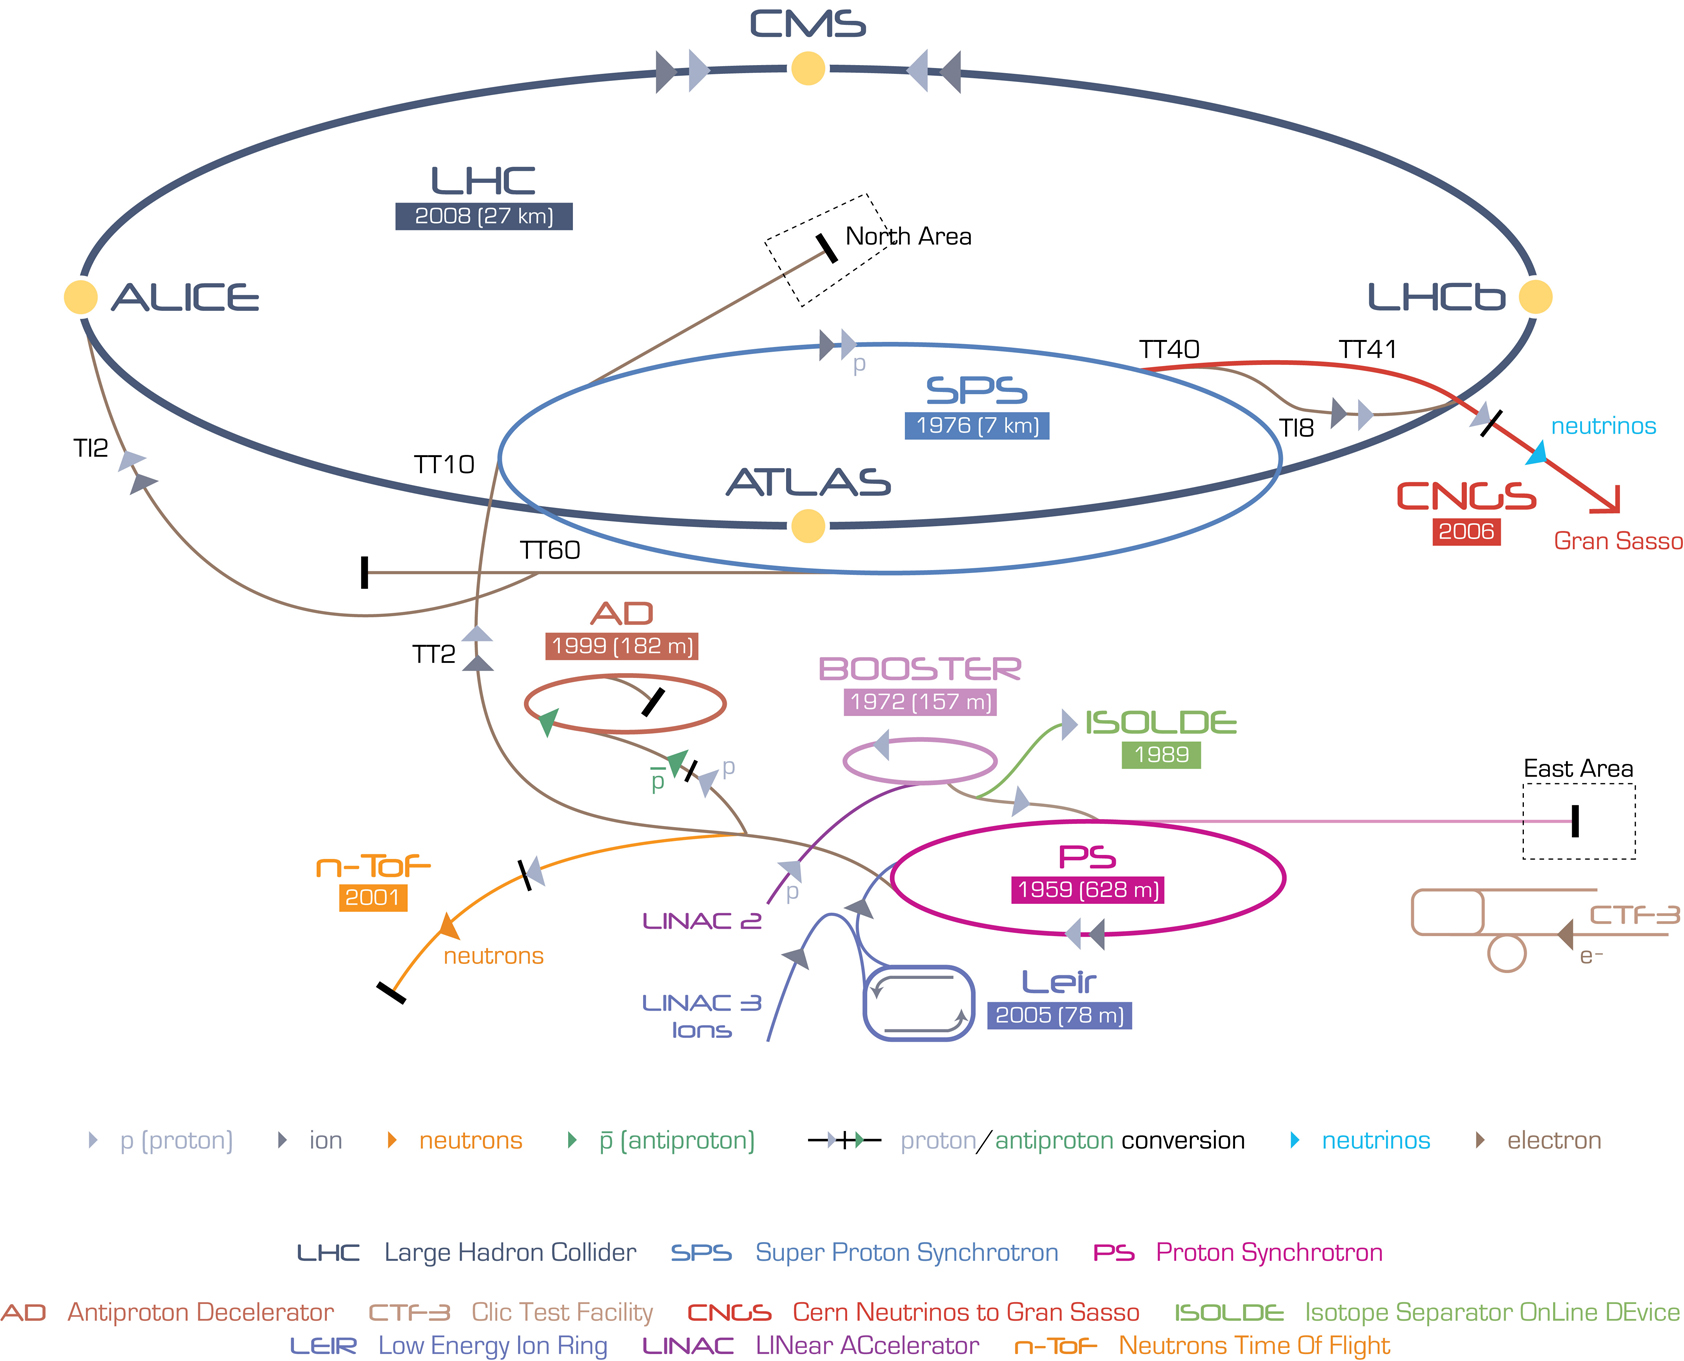
\includegraphics[width=0.75\textwidth]{figures/Cern-Accelerator-Complex.jpg}
 	\singlespace
 	\caption{Schematic diagram for the LHC experiment at CERN. Retrieved from \cite{LHC-schematic}.}
 	\label{fig:lhcdia}
 \end{figure}

 According to Einstein's famous equation $E=mc^{2}$, energy and mass are interchangeable. Therefore in order to produce heavy particles, a large amount of energy is required. The LHC was designed to produced highly energetic proton-proton, lead-proton or lead-lead beam collisions in which a variety of elementary particles can be produced.

 Therefore, the two most important features of a particle accelerator are its center of mass energy and its instantaneous luminosity ($\mathcal{L}$). The latter provides a measurement of the number of collisions that can be produced in the accelerator per squared centimeter and per second.

For a given process, the number of interactions (N) is the product of $\mathcal{L}$ integrated over the data taking time period and the cross section for the process in question ($\sigma_{ref}$):

\begin{equation}
N = \sigma_{ref}\int\mathcal{L}(t)dt
\end{equation} 

Now, the beams circulating the LHC ring are not continuous streams of particles, but rather trains of regularly spaced proton bunches. The experiment was designed to operate with 2,808 bunches of protons per beam, containing about $1.5\times10^{11}$ protons per bunch separated by 25 ns, corresponding to a collision frequency of 40 MHz. 

The LHC was planned to start in September 2008, but due to an incident damaging the machine, this was not the case. The startup was delayed until Nivember 23, 2009. Through its 2010-2011 run, the LHC operated at a center-of-mass energy of 7 TeV. Then in 2012, the energy was increased to 8 TeV, and again to 13 TeV in 2015, after a shutdown in 2013 that lasted two years.


\section{The CMS Detector}

The central feature of the CMS apparatus is a superconducting solenoid of 6m internal diameter, providing a magnetic field of 3.8 T. The solenoidal volume contains a silicon pixel and strip tracker, a lead tungstate crystal EM calorimeter. Each layer of the detector exploits a property of the particle to be detected to measure its energy or its momentum. 
An unusual feature of the CMS detector is that instead of being built on site like other giant detectors of the LHC experiment, it was constructed in 15 sections at ground level before being lowered into an underground cavern near Cessy in France and reassembled. The complete detector is 21 meters long, 12 meters wide and 15 meters high.

The goals of the physics program range from studying the SM (including the Higgs boson) to searching for extra dimensions and particles that could make up dark matter. It even has a very successful heavy ion program.

The layout of the detector can be seen in Figure \ref{fig:cmsdia}. The following sections will describe each of the sub-detectors and its properties.

 \begin{figure}[H]
 	\centering
 	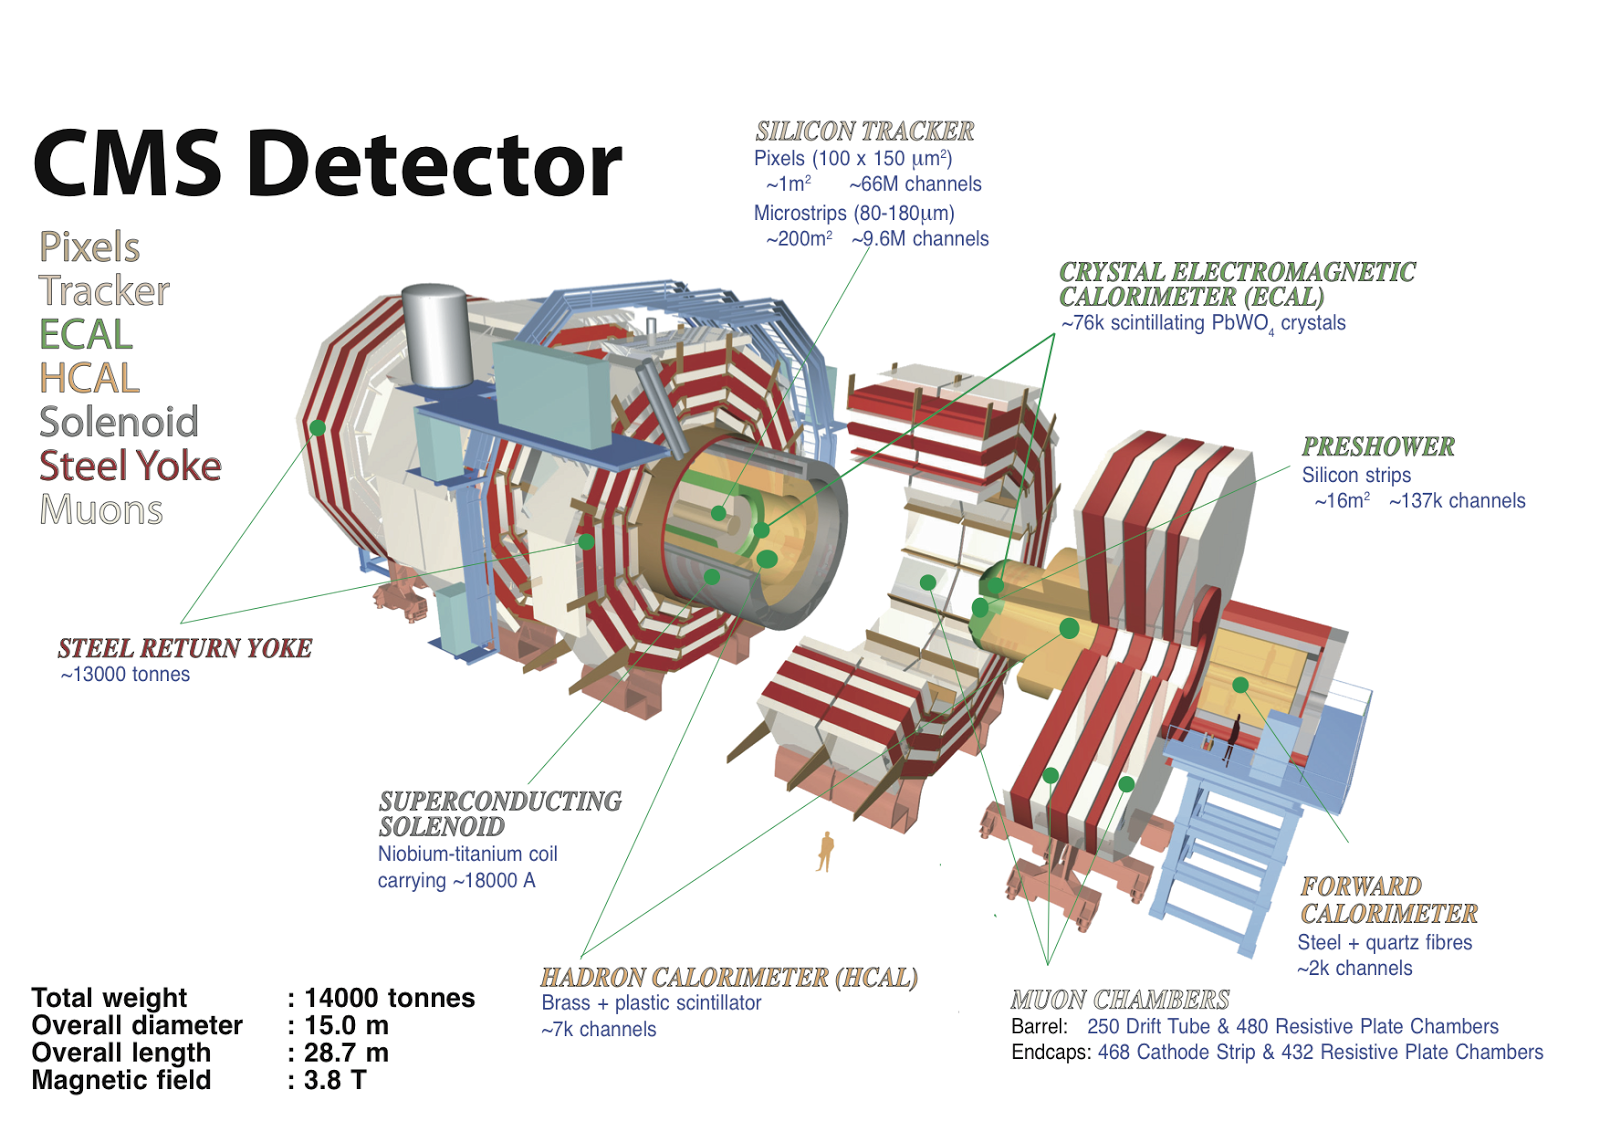
\includegraphics[width=0.85\textwidth]{figures/cms_whole.png}
 	\singlespace
 	\caption{Schematic diagram for the CMS experiment with its sub-detector systems and a person for scale. Retrieved from \cite{CMS-schematic}.}
 	\label{fig:cmsdia}
 \end{figure}

 \subsection{Coordinate System}

 The CMS experiment uses a right-handed coordinate system, with the origin at the nominal collision point, the $x-axis$ pointing to the center of the LHC ring, the $y-axis$ pointing up (perpendicular to the LHC plane), and the $z-axis$ along the anticlockwise beam direction. The polar angle($\theta$) is measured from the positive $z-axis$ and the azimuthal angle($\phi$) is measured from the positive $x-axis$ in the $x-y$ plane. The radius($r$) denotes the distance from the $z-axis$ and the pseudorapidity$(\eta)$ is defined as $\eta=-log[tan(\theta \ 2)]$. $\eta$ is preferently used by particle physicists to measure forward-ness of particles in the detector since any differences in this coordinate are invariant under boosts in the $z-$direction and particle production is roughly uniform in $\eta$. See Figure \ref{fig:cmscor} for reference.

  \begin{figure}[H]
 	\centering
 	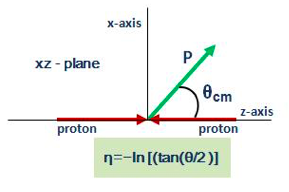
\includegraphics[width=0.5\textwidth]{figures/corsym.png}
 	\singlespace
 	\caption{Diagram for the CMS detector coordinate system.}
 	\label{fig:cmscor}
 \end{figure}

 \subsection{Tracker and Pixel Detector}
 Momentum analysis in CMS makes use of the magnetic field provided by its super-conducting solenoid around which the entire experiment is built. The tracker sub-detector is not only able to measure the momentum of charged particles but also determines their direction at their production vertex.

 The Tracker is the inner most layer of the detector and receives the highest volume of particles and therefore the construction materials were carefully chosen to resist radiation. It consists of a subsystem made entirely of silicon: the pixels, at the very core of the detector and dealing with the highest intensity of particles, and the silicon micro-strip detectors that surround it. In total, the sub-detector is 5.8 long and 2.5 m in diameter with an ability to measure the momentum of charged particles in the region $|\eta|<$ 2.5. Figure \ref{fig:cmstracker} shows the layout of the tracker and its subsystems.

   \begin{figure}[H]
 	\centering
 	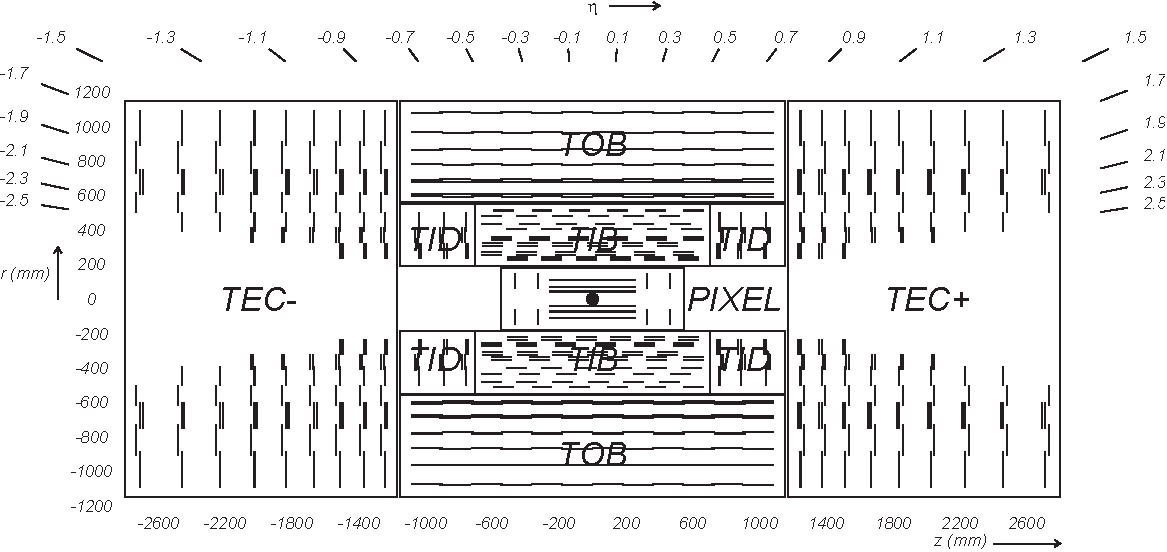
\includegraphics[width=0.9\textwidth]{figures/CMS_tracker.pdf}
 	\singlespace
 	\caption{Layout of the CMS detector tracker with subsystems labeled.}
 	\label{fig:cmstracker}
 \end{figure}

The pixel detector is made up of three barrel layers, called BPIX, and two endcap layers called the FPIX. The BPIX contains 48 million pixels and the FPIX contains another 18 million pixels. In totral it consists of 1440 hybrid silicon detector modules, each with a dimension of $100 \times 150 \mu m^{2}$. The small pixel size enables track resolutions of 10$\mu m$ in the transverse plane and 20$\mu m$ in the $z$-direction. The pixel detector is what gives CMS its exccellent secondary vertex tagging ability in addition to producing seed tracks for the strip tracker and the high level trigger.

Likewise, the silicon strip detector is made up of four subsystems. The Tracker Inner Barrel (TIB) has four layers of 320 $\mu m$ strips. At each end of the TIB is a three-layer Tracker Inner Disks (TID), which contains strips of the same thickness. The Tracker Outer Barrel (TOB) is the six layer system which surrounds the TIB/TID. The first four layers of the TOB use 500$\mu m$ thick strips, and the last two layers use 122 $\mu m$ thick strips. The Tracker EndCaps (TEC) are on either side of the previous setup and contain nine disks with up to seven layers of strips. These estrips are 320 $\mu m$ thick in the inner four rings and 500 $\mu m$ in the outer three rings. In total, the strip detector contains 9.3 million silicon strips.

 \subsection{Electromagnetic Calorimeter}

 The electromagnetic calorimeter (ECAL) is a homogeneous calorimeter made out of lead tungstate ($PbWO_{4}$) crystals totaling 75,848 units. The detector is divided up into two sections which provide a coverage of $|\eta| < 1.479$ in the barrel region (EB) and $1.479 < |\theta| < 3.0$ in two endcap regions (EE). There are also preshower detectors (PS) in each of the endcaps, in fornt of the EE, which cover a pseudorapidity range of $1.653 < |\eta| < 2.6$. Figure \ref{fig:cmsecal} shows the structure of the ECAL.

    \begin{figure}[H]
 	\centering
 	\includegraphics[width=0.9\textwidth]{figures/ECAL_transverse_Section.pdf}
 	\singlespace
 	\caption{A schematic of the CMS ECAL detector with its subsystems labeled.}
 	\label{fig:cmsecal}
	 \end{figure}

Each calorimeter cristal has a depth of 230 mm, which corresponds to 25.8 radiation lengths ($X_{0}$) for $PbWO_{4}$. The scintillation light produced in the crystals is read out by avalanche photodiodes (APDs), which produce approximately 4.5 photoelectrons per MeV at room temperature.

The energy resolution ($\sigma$) is typically parameterized according to

\begin{equation}
(\frac{\sigma_{E}}{E})^{2} = (\frac{N}{E[GeV]})^{2} + (\frac{S}{\sqrt{E[GeV]}})^{2} + C^{2}
\end{equation}

where $N$ is a term representing a contribution due to electronic and pileup noise, $S$ is the stochastic contribution to mis-measurement, and $C$ is the constant term. 


 \subsection{Hadron Calorimeter}

 The CMS hadron calorimeter (HCAL) is a sampling calorimeter, meaning it finds a particle's position, energy and arrival time using alternating layers of "absorber" and fluorescent "scintillator" materials that produce a rapid light pulse when the particle passes through. Special optic fibers collect up this light and feed it into readout boxes where photodetectors amplify the signal. Then the amount of light in a given region is summed up over many layers of tiles in depth, called a "tower", this total amount of light is a measure of a particle's energy. The HCAL is organized into barrel (HB and HO), endcap (HE), and forward (HF). There are 36 barrel "wedges", each weighting 26 tonnes. These form the last layer of detector inside the magnetic coil whilst a few additional layers, the outer barrel (HO), sit outside the coil, ensuring no energy leaks ouut the back of the HB undetected. Similarly, 36 endcap wedges measure particle enrgies as they emerge through the ends of the solenoid magnet.

 Lastly, the two hadronic forward calorimeters (HF) are positioned at either end of CMS, to pick up the myriad particles coming out of the collision region at shallow angles relative to the beam line. These receive the bulk of the particle energy contained in the collision so must be very radiation resistant and use different materials than the other parts of the HCAL.

 Figure \ref{fig:cmshcal} shows the structure and position of the HCAL subsystems. 

     \begin{figure}[H]
 	\centering
 	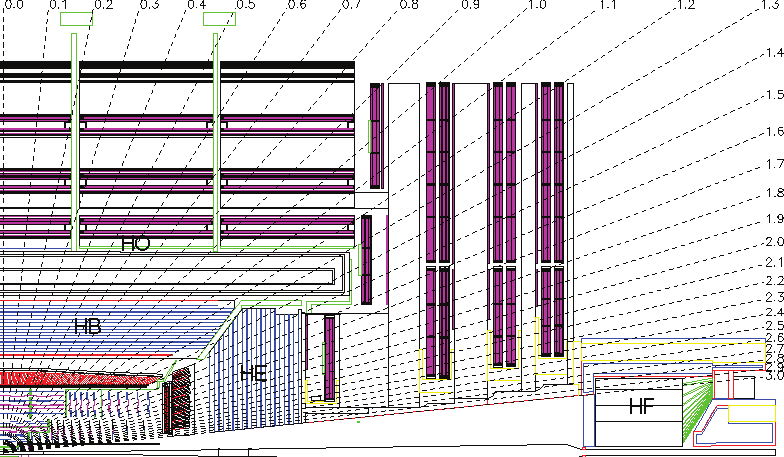
\includegraphics[width=0.9\textwidth]{figures/HCAL_subdet.pdf}
 	\singlespace
 	\caption{Structure and position of the CMS HCAL sub-detector systems.}
 	\label{fig:cmshcal}
	 \end{figure}

Combined, the ECAL and HCAL can measure the energy deposited by a charged pion with a resolution of $\sigma/E\approx100\%/\sqrt{E[GeV]}\oplus5\%$, where $E$ is the jet energy.

 \subsection{Solenoid}

 The CMS magnet is the central device around which the experiment is built, with a 4T tesla magnetic field, which is 100,000 times stronger than that of Earth.

 Its job is to bend the paths of charged particles emerging from high-energy collisions in the LHC. The higher momentum particles get their path curve less than the lighter ones, and as a result, curvature is an important tool for momentum measurements. 

 CMS strong magnetic field, combined with the high-precision position measurements in the tracker and muon detectors, allows for accurate measurement of the momentum of high-energy particles.

 The CMS solenoid magnet is made of coils of wire that produce a uniform magnetic field when electricity flows through them. Also, it is superconducting, the largest ever built, with a weight of 12,000 tonnes. In order for it to be superconducting, it needs to be colled down to -268.5 C, which is a degree warmer than outer space.

 The tracker and calorimeter detectors fit inside the magnet whilst the muon detectors are interleaved with a 12-sided iron structure that surrounds the magnet coils and contains and guides the field. Made up of three layers, this "return yoke" reaches out 14 metres in diameter and also acts as a filter, allowing through only muons and weakly interacting particles such as neutrinos. The enormous magnet also provides most of the experiment's structural support, and must be very strong itself to withstand the forces of its own magnetic field.


 \subsection{Muon System}
 After its magnet, the main feature of the CMS experiment is its capability of detecting muons. Since they can penetrate several meters of iron without interacting, gas-ionization detector chambers were placed at the very edge of the experiment embedded in the steel flux-return yoke in order to detect them. This allows for a pseudorapidity coverage of $|\eta| < 2.4$.

 The muon system consists of 1400 muon chambers which can be classified into three categories, according to the technology used: 250 drift tubes (DTs), 540 cathode strip chambers(CSCs), and 610 resistive plate chambers(RPCs).

 The barrel region of the detector contains DT's and RPCs, while the endcap region contains CSCs and RPCs. The layout of the muon system can be seen in Figure \ref{fig:cmsmuonsys}. 

    \begin{figure}[H]
 	\centering
 	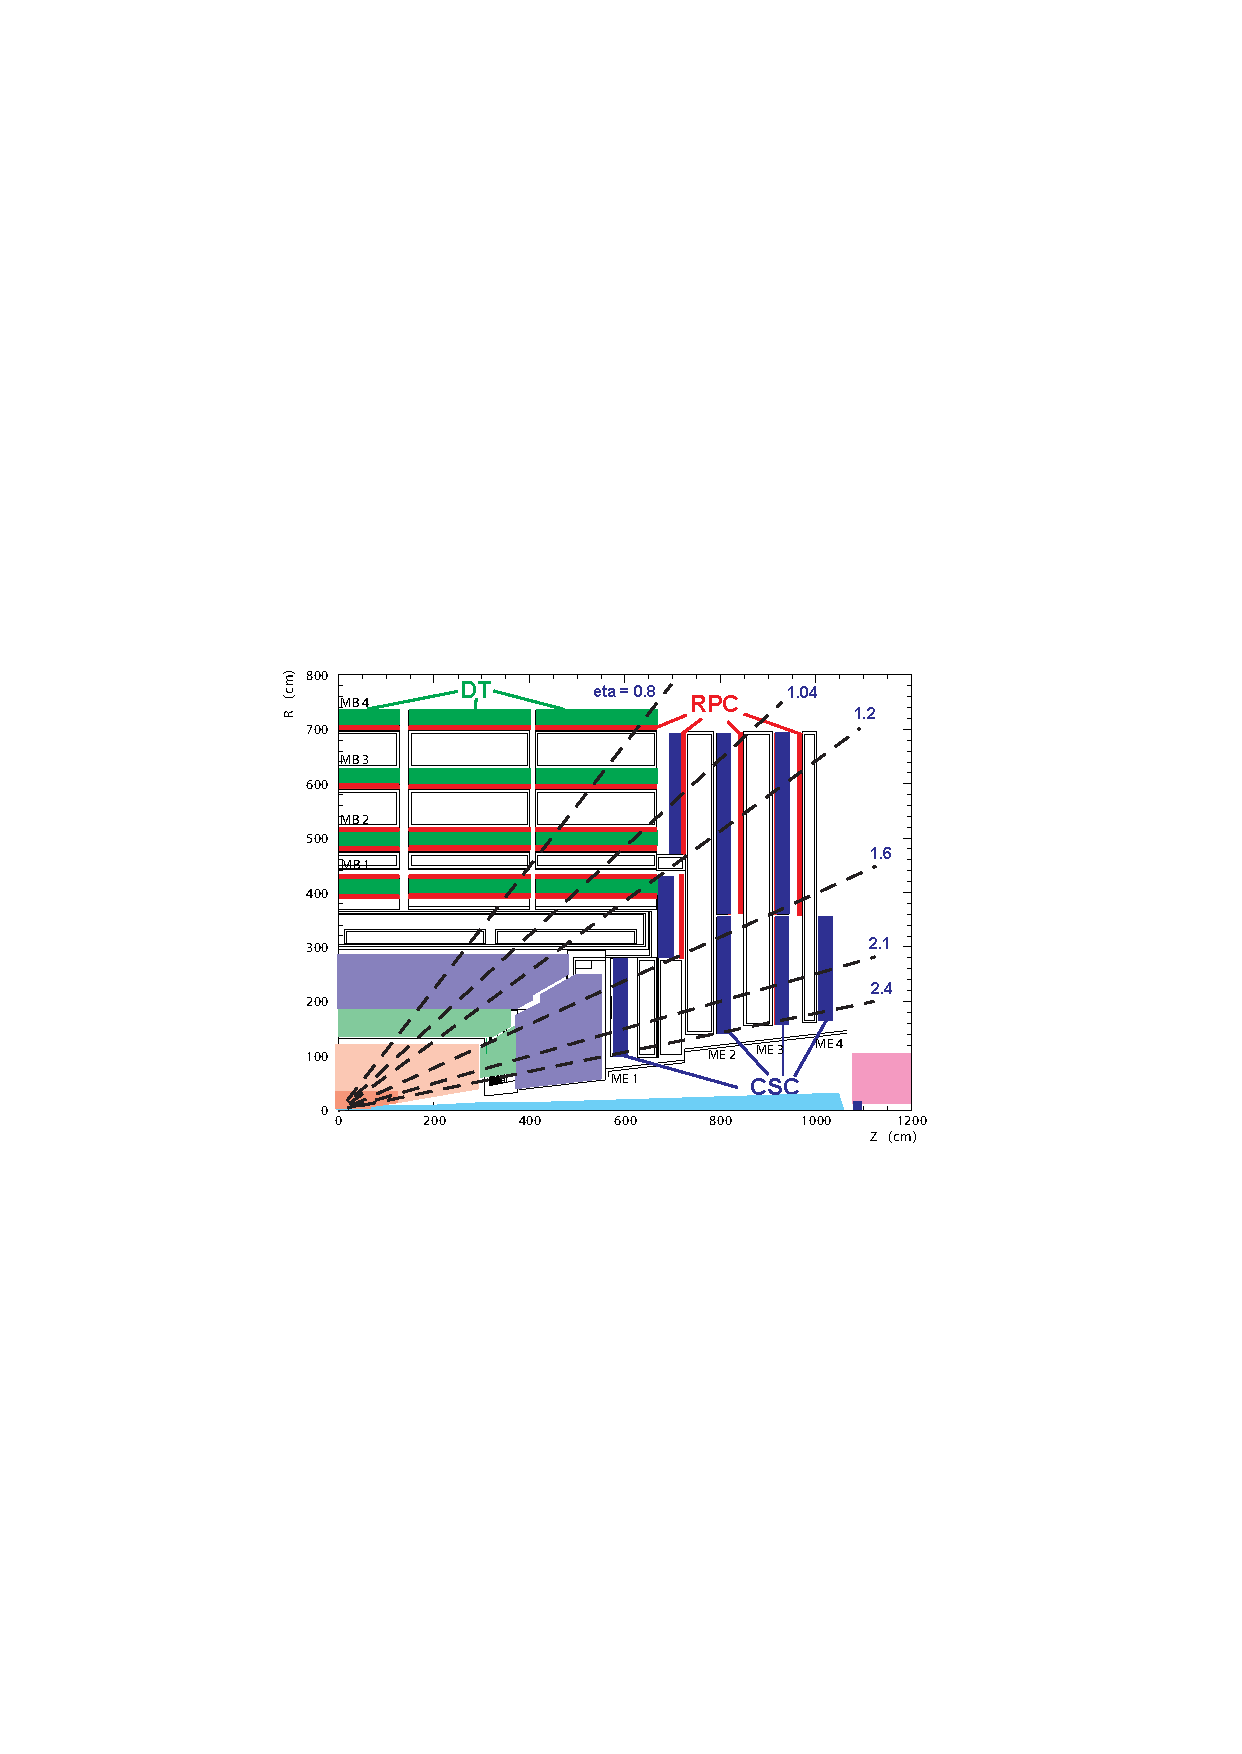
\includegraphics[width=0.9\textwidth]{figures/CMS_muon_system.pdf}
 	\singlespace
 	\caption{Layout of the CMS muon system.}
 	\label{fig:cmsmuonsys}
	\end{figure}

The four muon DT stations sitting outside the magnet coil are interleaved with the
iron "return yoke" (shown in red in Figure \ref{fig:cmsmuchambers}, for the barrel region), which not only returns the flux from the solenoid, but also shields the muon chambers from hadrons. 

    \begin{figure}[H]
 	\centering
 	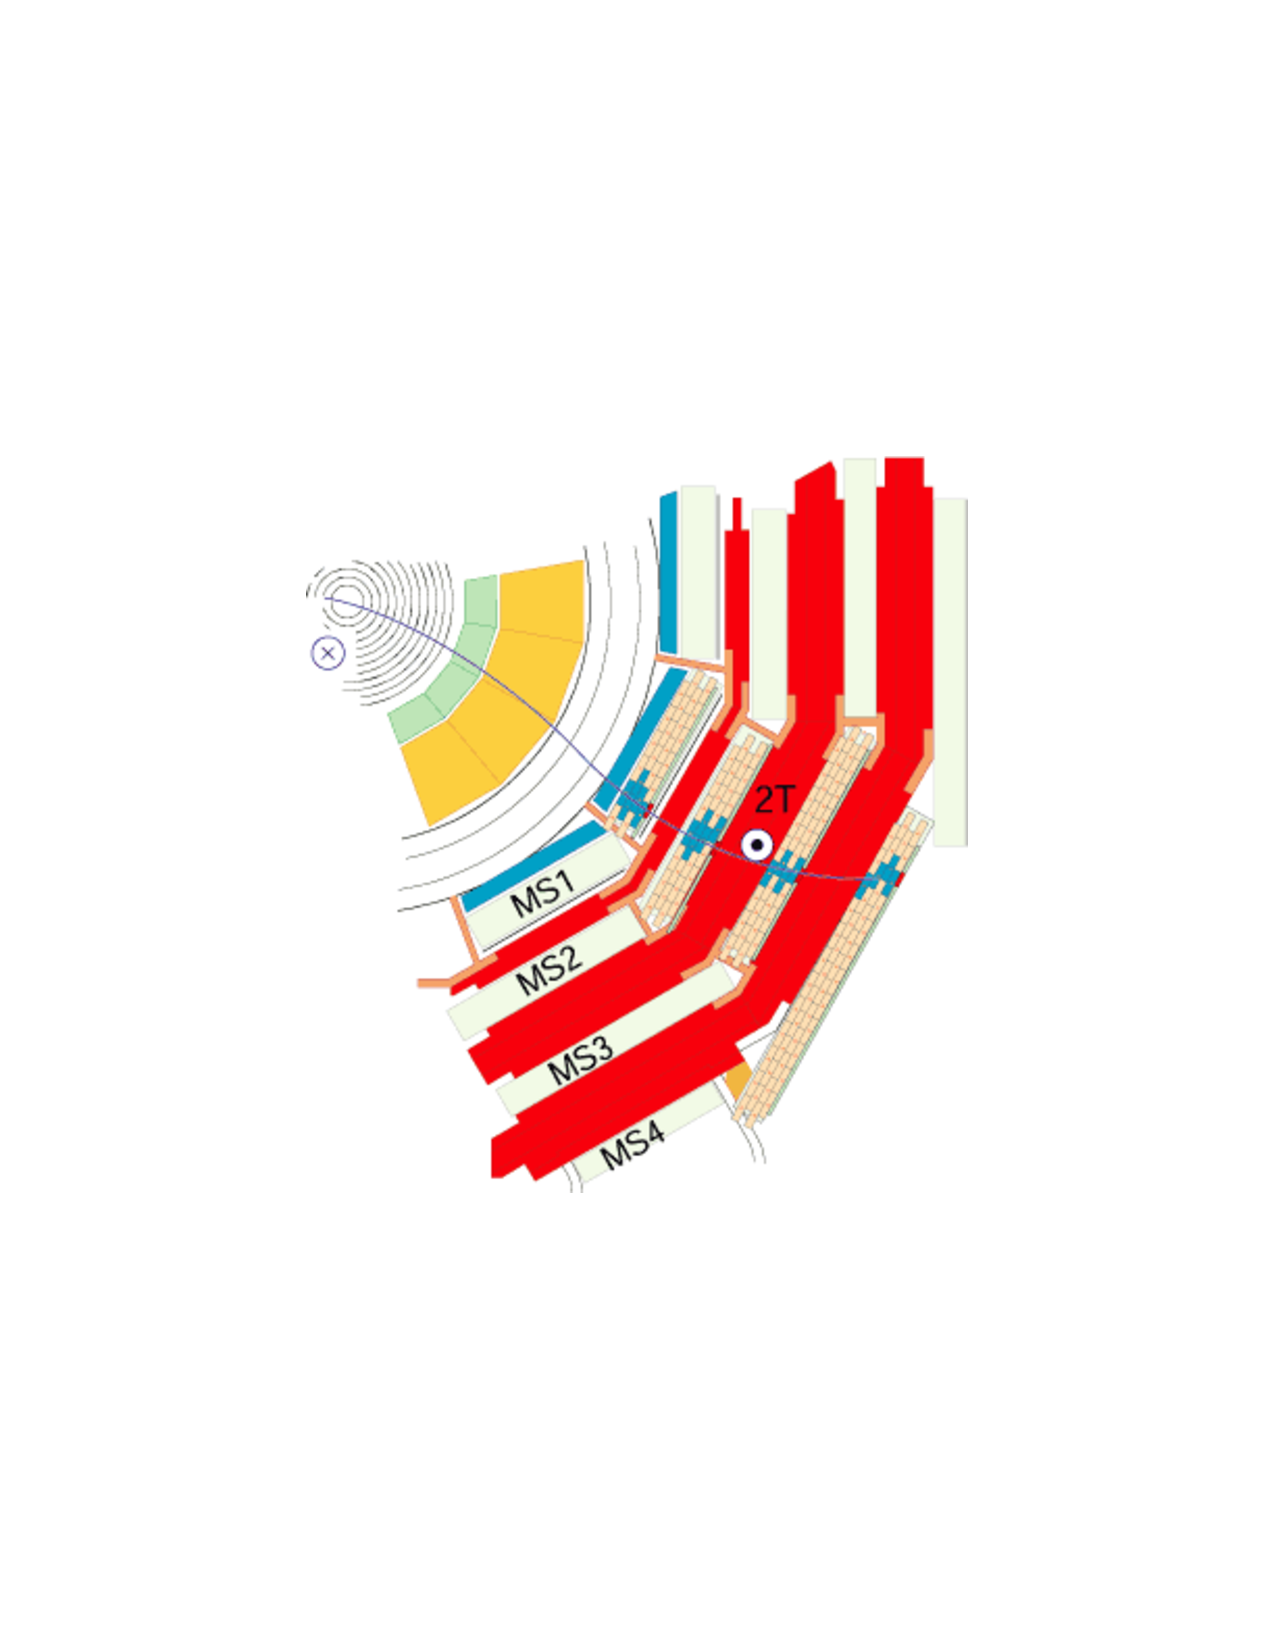
\includegraphics[width=0.9\textwidth]{figures/MuStations.pdf}
 	\singlespace
 	\caption{A muon, in the plane perpendicular to the LHC beams, leaves a curved trajectory in four layers of muon detectors or stations.}
 	\label{fig:cmsmuchambers}
	\end{figure}

The CSCs track the particle's position and allow for triggering, while the RPCs form a redundant trigger system, which quickly decides to keep the acquired muon data or not. Because of the many layers of detector and different specialties of each type, the system is naturally robust and able to filter out background noise.

The muon system on its own has a resolution of 15-40$\%$ depending on $\eta$. Matching muons to tracks measured in the silicon tracker results in a relative transverse momentum resolution for muons with 20$< p_{T} < $ 100 GeV of 1.3-2.0$\%$ in the barrel and better than 6$\%$ in the endcaps. The $p_{T}$ resolution in the barrel is better than 10$\%$ for muons up to 1 TeV \cite{Chatrchyan:2012xi}.


 \subsection{Trigger}
 When CMS is performing at its peak, about one billion proton-proton interactions will take place every second inside the detector. In order to record only those events generated from energetic, head-on collisions, a "trigger" system was implemented.

Level 1 of the trigger is an extremely fast, hardware based process that looks for simple signs of interesting physics, e.g. particles with a large amount of energy or in unusual combinations. The L1 trigger selects events at a rate of around 100 kHz within a time interval of 4$\mu$s. The next step is the High Level Trigger (HLT), which combines the information from different parts of the detector to recreate the entire event and send it to a farm of more than 1000 computers to filter even more events, reducing the event rate to less than 1 kHz before recording them on tape.

\subsection{Luminosity Measurement}

Bsides measuring the kinematics of each of the particles traversing the detector, CMS must also measure the instantaneous luminosity delivered by the LHC. Both the pixel detector, and the HF are able to measure the luminosity to varying degrees of accuracy.

The Van der Meer (VdM) scan method measures the size and shape of the interaction region of the colliding beams. This is achieved by displacing the beams in the x and y- (transverse) planes and measuring the relative interaction rates as a function of the transverse beam separation. For Gaussian beams, the luminosity as a function of the transverse displacement ($\delta u$) can then be expressed as:  

\begin{equation}
\mathcal{L}(\delta u) = \mathcal{L}_{0} exp[-\frac{\delta u^{2}}{2\sigma_{u}^{2}}]
\end{equation}

where 

\begin{equation}
\mathcal{L}_{0} = \frac{N_{1}N_{2}fN_{b}}{2\pi\sqrt{(\sigma_{1x}^{2}+\sigma_{2x}^{2})(\sigma_{1y}^{2}+\sigma_{2y}^{2})}}
\end{equation}

and $\sigma_{u} = \sqrt{\sigma_{1u}^{2}+\sigma_{2x}^{2}}$ with $u=x,y$ for each separation plane, $N_{b}$ the number of colliding bunches and $f$ the revolution frequency.

A fit of the measured interaction rates as a ufnction of the reparation will allow to determine the effective beam size as well as the maximum achievable collision rate ($\dot{N}$)

\begin{equation}
\dot{N} = \mathcal{L}\sigma
\end{equation}

In practice, the scans are performed by moving the beams step-wise across each other in the two transverse plane.

% Notice that the title of this section is long - much longer than the others. When you have long section titles, this template takes care of double spacing the lines in the title. If the title is long to fit in the table of contents, the template will single space the title.

% \section{Yet Another Table}

% Another table is placed here to show the effect of having tables in multiple sections. The list of tables should still double space between table titles, while single spacing long table titles.

% %Fix table labeling.
% \begin{table}[h!]
% 	\centering
% 	\begin{tabular}{|l|l|}
% 		\hline
% 		Dates & Attendance  \\ \hline
% 		August 8-10, 2008 & 3,523  \\ \hline
% 		August 14-16, 2009 & 4,003 \\ \hline
% 		July 9-11, 2010 & 5,049 \\ \hline
% 		August 5-7, 2011 & 6,891  \\ \hline
% 		August 10-12, 2012 & 9,464  \\ \hline
% 		August 16-18, 2013 & 11,077  \\ \hline
% 		July 18-20, 2014 & 14,686 \\ \hline
% 		July 31-August 2, 2015 & 18,411  \\ \hline
% 	\end{tabular}
% 	\caption{San Japan attendance. Data is taken from \cite{ANCONS}. I intentionally make the title of this table long so the single space effect is seen in the list of tables.}
% \end{table}

% You may be wondering why San Japan was chosen. There are a few reasons as to why I did this:

% \begin{enumerate}
% \item It is one of the fastest-growing anime conventions in Texas.
% \item Filler.
% \item I wanted a good variety of table examples.
% \item Because conventions are cool.
% \end{enumerate}

% The \textit{enumerate} environment was used to generated an ordered list above.

% \section{Section Test Example}
% We insert another figure here, just for kicks.

% \begin{figure}[h!]
% 	\centering
% 	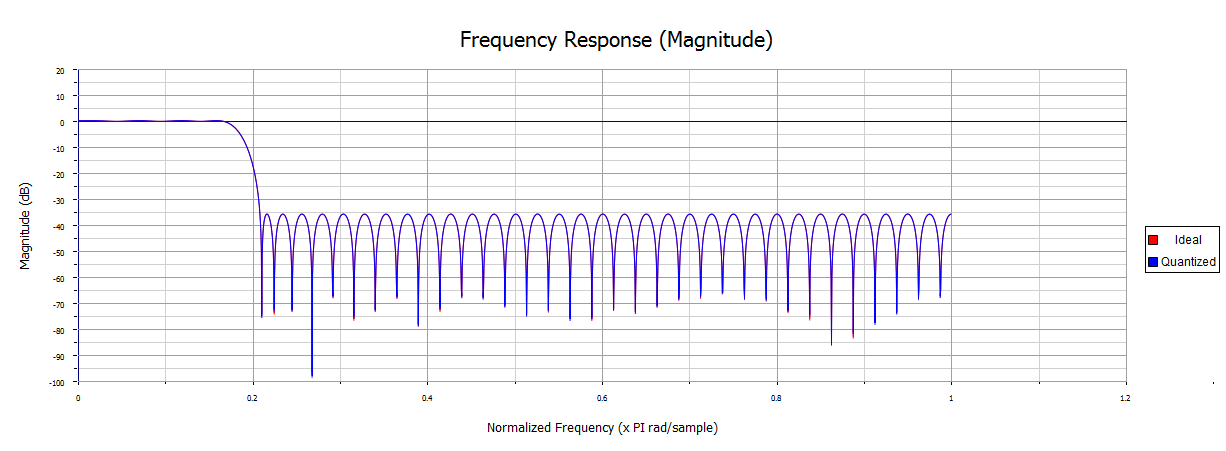
\includegraphics[width = 6.0in]{LowPass_Filter_Design.png}
% 	\caption{A low pass filter design.}
% \end{figure}

% \subsection{Filler, Filler, Filler}

% This section has filler text. These words serve no meaning except to fill a few lines in the document. This section has filler text. These words serve no meaning except to fill a few lines in the document. This section has filler text. These words serve no meaning except to fill a few lines in the document.

% \begin{figure}[h!]
% 	\centering
% 	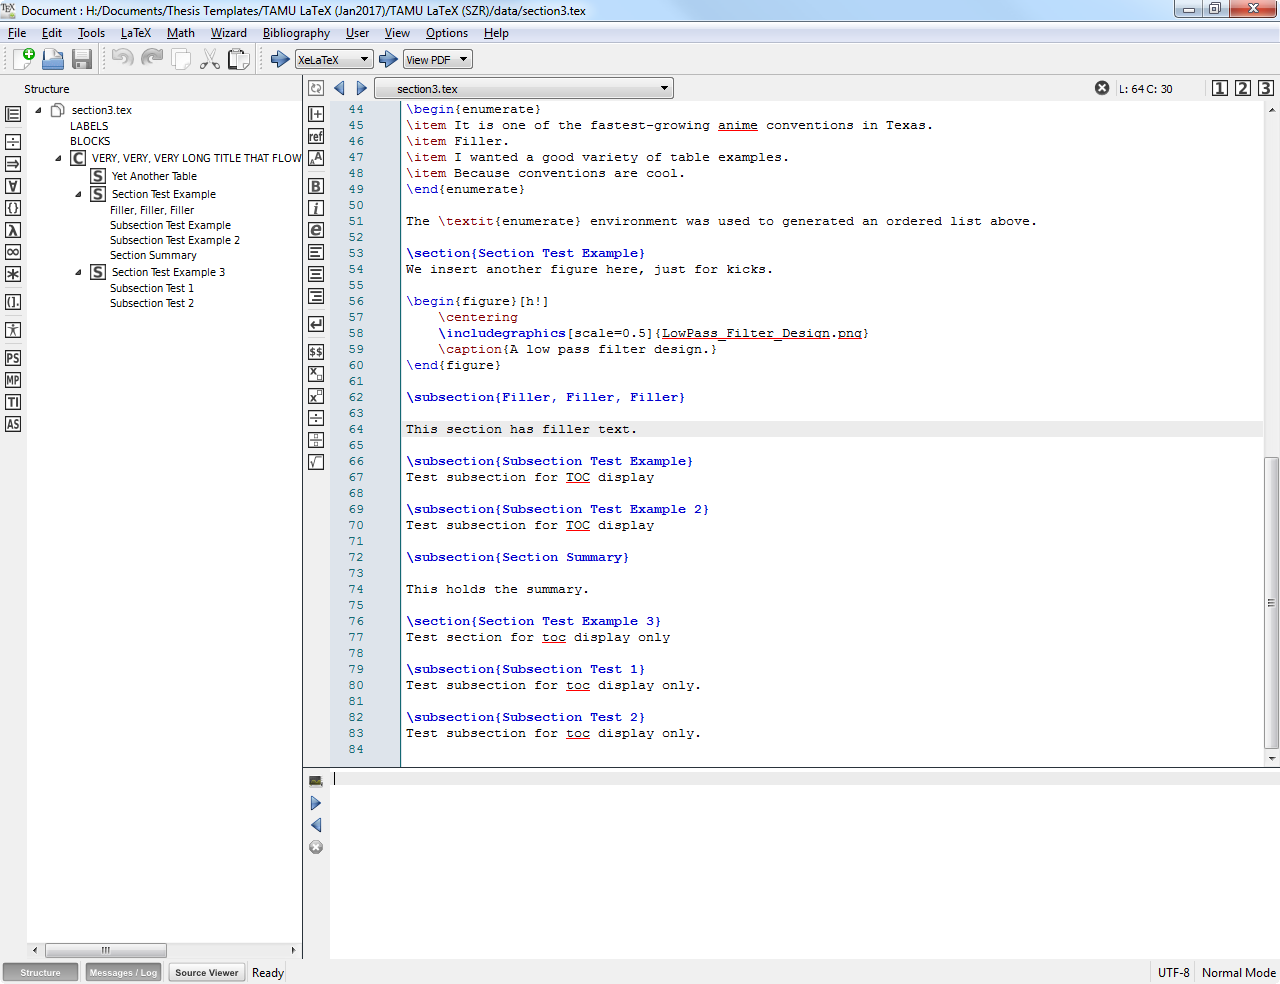
\includegraphics[width=3.75in]{Workspace1.png}
% 	\caption{A typical Texmaker workspace in Windows 7. The right sidebar displays the current file's structure according to the subsections in place.}
% \end{figure}

% This section has filler text. These words serve no meaning except to fill a few lines in the document. This section has filler text. These words serve no meaning except to fill a few lines in the document. This section has filler text. These words serve no meaning except to fill a few lines in the document. This section has filler text. These words serve no meaning except to fill a few lines in the document. This section has filler text. These words serve no meaning except to fill a few lines in the document. This section has filler text. These words serve no meaning except to fill a few lines in the document.

% \begin{figure}[h!]
% 	\centering
% 	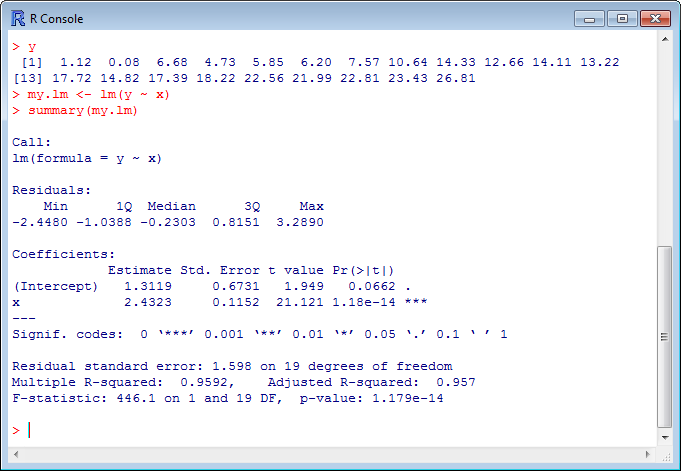
\includegraphics[width=3.5in]{Rachl1.png}
% 	\caption{Some commands in R.}
% \end{figure}

% \subsection{Subsection Test Example}
% Test subsection for TOC display

% \subsection{Subsection Test Example 2}
% This section has filler text. These words serve no meaning except to fill a few lines in the document. This section has filler text. These words serve no meaning except to fill a few lines in the document. This section has filler text. These words serve no meaning except to fill a few lines in the document.

% \begin{figure}[h!]
% 	\centering
% 	
\includegraphics[scale=0.85]{TAM_Logo1.png}
% 	\caption{The logo of a familiar university.}
% \end{figure}

% \begin{figure}[!h]
% 	\caption{Yet another blank float that has no purpose. This is only to test the appearance of the Lists of Figures and the List of Tables.}
% \end{figure}

% \subsection{Section Summary}
  
% This holds the summary. Well, not really a summary - there was a lot of filler in this section.

% \begin{figure}[h!]
% 	\centering
% 	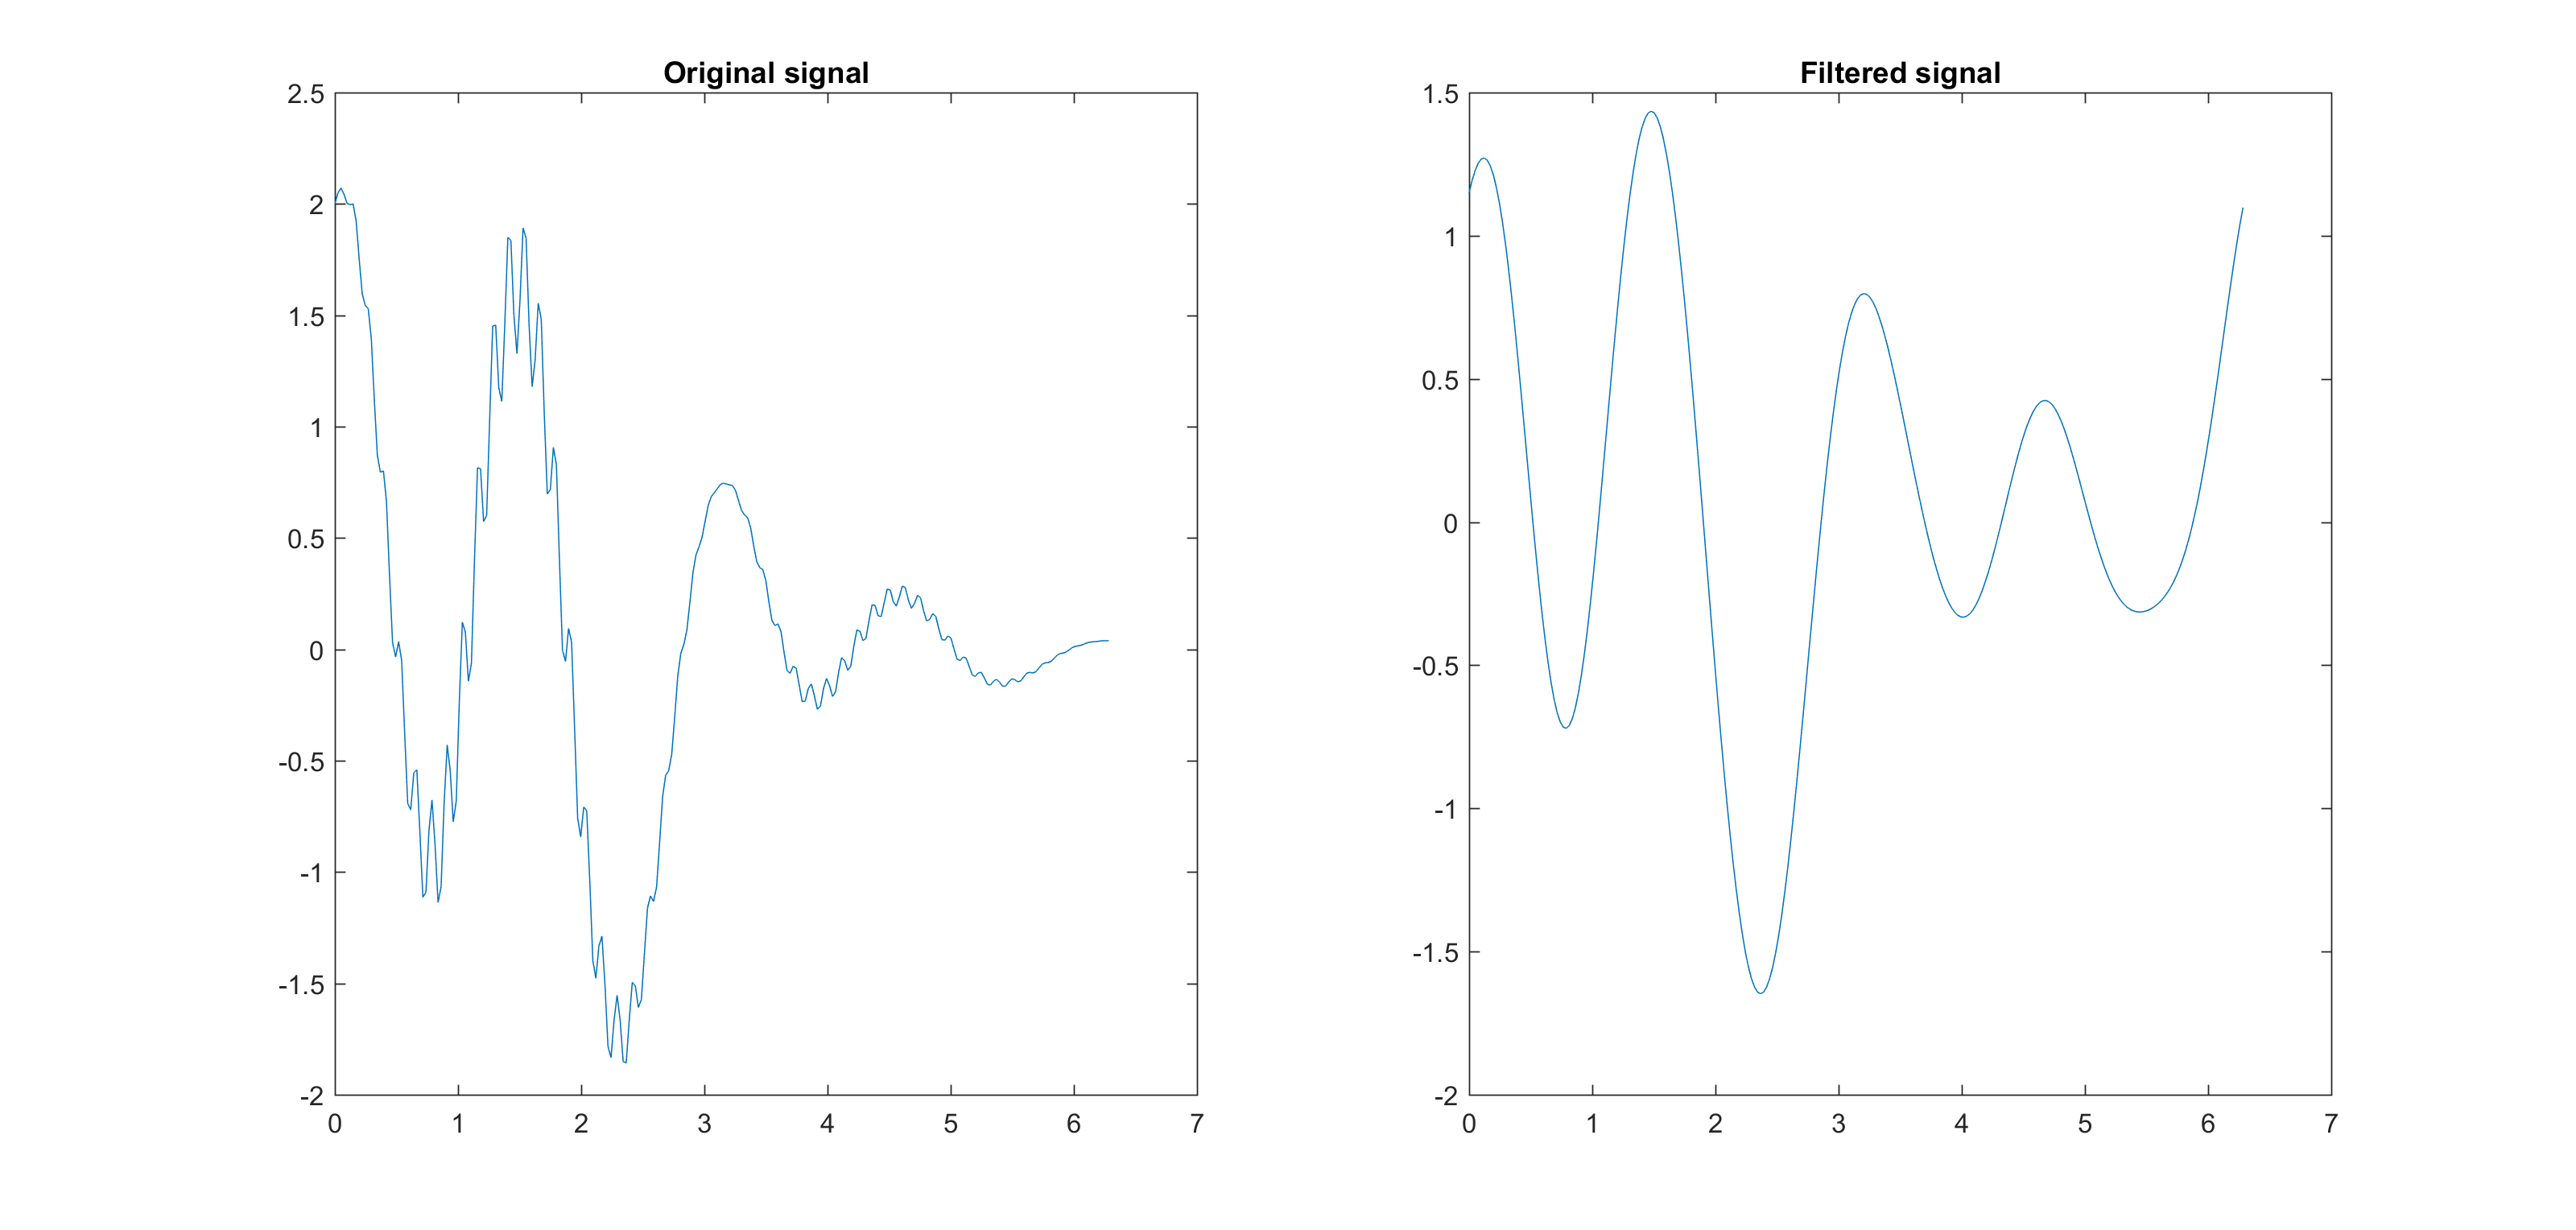
\includegraphics[width=6.5in]{Filter1.png}
% 	\caption{A signal and the result after a basic filter. The FFT was used to create the plot on the right.}
% \end{figure}

% \section{Section Test Example 3}
% Test section for toc display only.

% \begin{figure}[!h]
% 	\caption{There is nothing to see here.}
% \end{figure}

% \begin{figure}[!h]
% 	\caption{There is another float here. I wonder what could be here? Guess what? Nothing! There is no material in this float.}
% \end{figure}

% \subsection{Subsection Test 1}
% Test subsection for toc display only.

% \subsection{Subsection Test 2}
% Test subsection for toc display only.
%%%%%%%%%%%%%%%%%%%%%%%%%%%%%%%%%%%%%%%%%%%%%%%%%%%%
%
%  New template code for TAMU Theses and Dissertations starting Fall 2016.  
%
%
%  Author: Sean Zachary Roberson
%  Version 3.17.09
%  Last Updated: 9/21/2017
%
%%%%%%%%%%%%%%%%%%%%%%%%%%%%%%%%%%%%%%%%%%%%%%%%%%%
%%%%%%%%%%%%%%%%%%%%%%%%%%%%%%%%%%%%%%%%%%%%%%%%%%%%%%%%%%%%%%%%%%%%%%
%%                           SECTION IV
%%%%%%%%%%%%%%%%%%%%%%%%%%%%%%%%%%%%%%%%%%%%%%%%%%%%%%%%%%%%%%%%%%%%%



\chapter{EVENT RECONSTRUCTION \label{cha:eventreco}}
In the CMS detector, collisions happen in a small longitudinal region near the center called the luminous region or interaction region. Collisions themselves are not recorded, only the particles that get created. The origin of one or more new particles is called a vertex. An event is the set of particle measurements in the detector associated to a single beam-beam crossing. It is the job of the reconstruction software to process the raw information and identify physics objects for a given event.

 \begin{figure}[H]
 	\centering
 	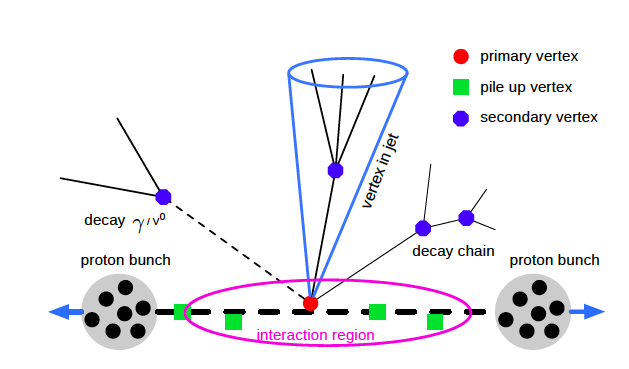
\includegraphics[width=0.75\textwidth]{figures/eventvertex.png}
 	\singlespace
 	\caption{Schematic diagram for an event at the LHC.}
 	\label{fig:vertex}
 \end{figure}


\section{Data Acquisition}
The CMS Data Acquisition (DAQ) and trigger system was specifically designed to collect and analyze data at a rate of 40MHz, which corresponds to a 25 ns collision rate. Unfortunately, due the electronics system is only able to record a few hundreds of Hz of events. Therefore, events are filtered online by so-called trigger systems, so that only interesting events are written to disk. The collision triggering the readout is called the primary vertex, while other collisions from the beams are called pile-up. Secondary vertices refer to the other production points, when particles are created from decay or hard-scattering. This is shown in Figure \ref{fig:vertex}. Particles from the primary vertex usually have a high transverse momentum ($p_{T}$), making them interesting and easier to study.

\subsection{L1 Trigger and HLT}
 When CMS is performing at its peak, about one billion proton-proton interactions will take place every second inside the detector. In order to record only those events generated from energetic, head-on collisions, a "trigger" system was implemented.

Level 1 of the trigger is an extremely fast, hardware based process that looks for simple signs of interesting physics, e.g. particles with a large amount of energy or in unusual combinations. The L1 trigger selects events at a rate of around 100 kHz within a time interval of 4$\mu$s. The next step is the HLT, which combines the information from different parts of the detector to recreate the entire event and send it to a farm of more than 1000 computers to filter even more events, reducing the event rate to less than 1 kHz before recording them on tape.

\subsection{T1 sites and data storage}

CMS computing operates on a tiered computing structure. A Tier-0 computing center is located at CERN where the data is transferred form the HLT and a first set of reconstruction occurs. From there, it is transferred to one of seven Tier-1 computing centers located around the world. At the Tier-1 centers, a full reconstruction of the data is performed. Furthermore, there are 55 Tier-2 centers which can be accessed by the collaboration members for data processing and storage.

 \begin{figure}[H]
 	\centering
 	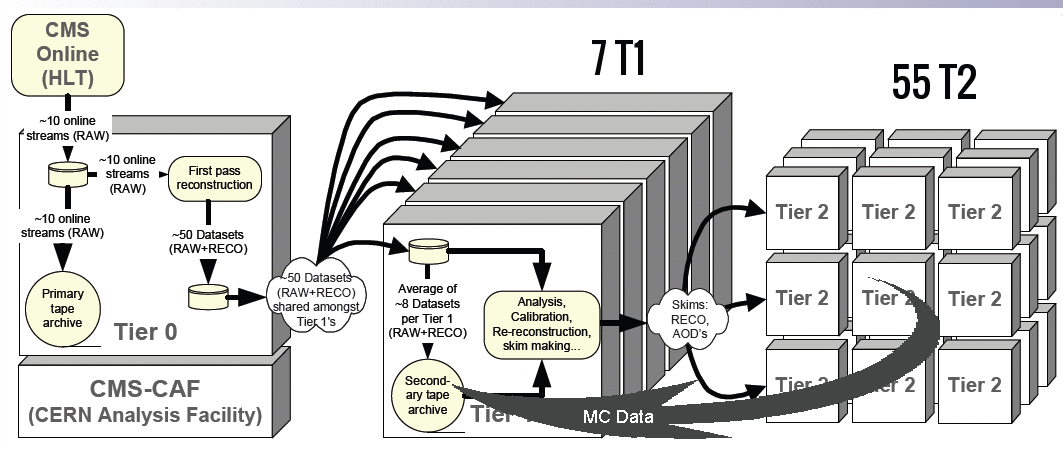
\includegraphics[width=0.75\textwidth]{figures/dataflowtiers_MC.png}
 	\singlespace
 	\caption{Flow of CMS detector data through the tiers. Reprinted from \cite{CMSdatatier}}
 	\label{fig:datatier}
 \end{figure}

 The data itself is also processed in three data tiers. The first layer of this is the RAW data, which is created by unpacking detector streams passed on from the L1 and HLT triggers, typically composed of measurements from the different calorimeters as well as some information provided by the L1 trigger. This RAW data is reconstructed into physics objects(i.e. muons, electrons, photons) that can be grouped later for further analysis. This step is called RECO, which is short for reconstruction and contains both the detector and physics object information. 

 After RECO, an \textit{analysis object data} (AOD) is formed from a subset of the RECO information. AOD objects are typically comprised of only high-level physics objects, making the files much smaller. This data format is usually the preferred one for physics analysis.



\section{Particle Flow Event Reconstruction}
\label{sec:track}

As mentioned in Section 2, CMS is one of the two general-purpose detectors at the LHC, and as such, it was designed based on the concept of cylindrical detection layers. In the previous section we described how data was managed and stored during the acquisition process. This section will focus on how physicists make sense of the raw detector information.  

 First, detector data is measured in the form of electronic signals, i.e. hits in the tracker or energy depositions in the calorimeters. Then, the trajectories of charged particles, or tracks, are reconstructed from the position hits in the detector. From the collection of tracks in an event, the primary and any secondary vertices are reconstructed. 

An optimal event description can be achieved by correlating the basic elements from all detector layers (tracks and clusters) to identify each final-state particle, and by combining the corresponding measurements to reconstruct the particle properties on the basis of this identification. At CMS, this approached is called \textit{particle-flow (PF) reconstruction}.

The reconstructed and identified individual particle list includes muons, electrons, photons, charged hadrons, as well as stable and unstable neutral hadrons. These particles can be non-isolated, and even originate from an intricate overlap of reconstructed charged particles, ECAL and HCAL energy clusters, and signals in the muon chambers.

Looking at Figure \ref{fig:cmsslice}, one can see that photons and neutral hadrons are in general identified by ECAL and HCAL clusters with no track link. No attempt is made to distinguish the various species of neutral and charged hadrons in the PF reconstruction. Electrons can be identified by a track and an ECAL cluster, with a momentum-to-energy ratio compatible with unity, and not connected to an HCAL cluster. Finally, muons and neutrinos would traverse the calorimeters with little or no interactions. While neutrinos would escape undetected, muons would be identified by a track in the inner tracker connected to a track in the muon detectors.

 \begin{figure}[h]
  	\label{fig:cmsslice}
 	\centering
 	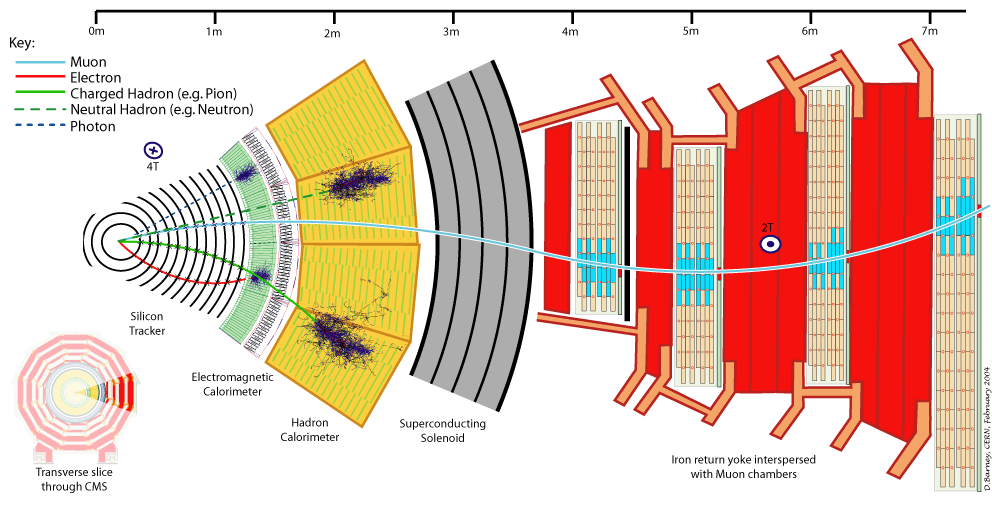
\includegraphics[width=0.75\textwidth]{figures/image005.png}
 	\singlespace
 	\caption{Cross-sectional view of the CMS detector with all of the sub-detectors labeled. The colored lines correspond to different particle types. Each particle interacts with different pieces of the detector and may or may not be bent by the magnetic field. Reprinted from \cite{CMSSlice}}
 \end{figure}

The PF concept was developed and used for the first time by the ALEPH experiment at LEP\cite{BUSKULIC1995481} and can now be used in hadron colliders due to the very fine spatial granularity of the detectors. In particular, CMS is very well suited for PF reconstruction due to its highly-segmented tracker,  a fine-grained ECAL, and an hermetic HCAL.

Also, the CMS magnet is large enough to accommodate the tracker and both the ECAL and HCAL, thereby minimizing the mount of material in front of the calorimeters. This particular feature is an advantage for PF reconstruction, as it eliminates the energy losses before the calorimeters caused by particles showering in the coil material and facilitates the link between tracks and calorimeter clusters.

\subsection{Iterative Tracking}

 The first step of the reconstruction process is referred to as local reconstruction and it consists of the clustering of \textit{zero-suppressed} signals above specified thresholds in pixel and strip channels into hits. The next step is track reconstruction, which refers to the process of using the reconstructed hits to obtain estimates for the momentum and position parameters of the charged particles responsible for the detector hits. 

 The tracking software at CMS\cite{TRK-11-001} is commonly referred to as the combinatorial Track Finder (CTF), which is an adaptation of the combinatorial Kalman Filter \cite{Billoir:1989mh},\cite{BILLOIR1990219},\cite{Mankel:1997dy}, which in turn is an extension of the Kalman filter\cite{Fruhwirth:1987fm} to allow pattern recognition and track fitting to occur in the same framework. The collection of reconstructed tracks is produced by multiple passes or iterations of the same CTF track reconstruction sequence, in a process called iterative tracking. 

The basic idea of iterative tracking is that the initial iteration seach for tracks that are easiest to find (e.g., of relatively large $p_{T}$, and produced near the interaction region). After each iteration, hits associated with tracks are removed, thereby reducing the combinatorial complexity, and simplifying subsequent iterations in a seach for more difficult classes of tracks (e.g., low $p_{T}$, or greatly displaced tracks).

Each iteration proceeds in four steps:

\begin{itemize}
	\item Seed generation which provides track candidates consisting of a few (2 or 3) hits. Seeds are generated in the innermost layers of the tracker and are commonly referred to as "proto-tracks".
	\item Track finding, which is based on a Kalman filter. It extrapolates the seed trajectories along the expected flight path of a charged particle, searching for additional hits that can be assigned to the track candidate.
	\item Track fitting. A module that is used to provide the best possible estimate of the parameters of each trajectory by means of a Kalman filter.
	\item Track selection. This step sets the quality flags and discards tracks that fails certain specified criteria.
\end{itemize}

A total of six iterations are used, each with different seed generation, $p_{T}$ and impact parameter requirements.

The first iterations have strict criteria in order to achieve a negligible small fake rate. Once the hits are associated with these tracks are removed, the seeding criteria is loosened. By doing this, tracking efficiency is increased. From iteration 4 and on, the constraints on the tracks closer to the interaction point are slowly relaxed. This allows for reconstruction of secondary charged particles created from photon conversions and nuclear interactions in the tracker volume.

\subsection{Calorimeter Clustering}
Clustering in the calorimeters is the process of grouping detector cells that register hits together to measure the energy and direction of stable neutral particles. Additionally, clustering seeks to separate the neutral particles from energy deposits associated with charged hadrons, reconstruct electrons (including all associated Bremsstrahlung photons), and measure the energy of charged hadrons for which tracks were not determined accurately. The clustering algorithm is performed separately in each sub-detector: ECAL barrel and endcap, HCAL barrel and endcap, and in the pre-shower.

The clustering proceeds via three steps\cite{CMS:2009nxa}:

\begin{enumerate}
	\item Identify 'cluster seeds'. These are defined as the cell in a calorimeter with a local maximum of energy (above some set threshold).
	\item Expand from the seed to grow 'topological clusters'. This is done by aggregating calorimeter cells that have at least one side in common with the seed cell, and also have an energy over a particular threshold.
	\item Repeat the process of cluster growing, now using new cells that are part of the cluster.
\end{enumerate}

In this sense, a "seed" gives rise to a "particle-flow cluster". If a cell is identified by two clusters, the energy is shared between the clusters according to the distance from the cell to the center of each cluster. The cluster energies and positions are iteratively determined as new cells are added to the cluster.

\subsection{Linking Tracks and Clusters}
Once the basic PF elements like the trajectories of charged particles in the inner tracker, electron and muon tracks, and calorimeter clusters are available, the next step in reconstructing a particle is the so-called \textit{link algorithm}.

 The link algorithm can test any pair of elements in the event. In order to prevent the computing time of the link algorithm from growing quadratically with the number of particles, the pairs of elements considered by the link procedure are restricted to the nearest neighbors in the ($\eta,\phi$) plane, as obtained with a $k$-dimensional tree\cite{Bentley1975MultidimensionalBS}. The specific conditions required to link two elements depend on their nature.

 If two elements are found to be linked, the algorithm defines a distance between these two elements, aimed at quantifying the quality of the link. The link algorithm then produces \textit{PF blocks} of elements associated either by a direct link or by an indirect link through common elements.

 The link between tracks and calorimeter clusters proceeds by extrapolating the last measured hit in the tracker to one of the three detectors\cite{CMS:2009nxa}:

 \begin{itemize}
 	\item The two layers of the pre-shower detector,
 	\item the ECAL, at a depth corresponding to the expected maximum of the electron shower profile,
 	\item the HCAL, to a depth corresponding to one interaction length.
 \end{itemize}

 The track is then linked to a cluster in these detectors if the extrapolated position is within the cluster boundaries. Additionally, to link Bremsstrahlung photons to their associated electron, tangents to the track are extrapolated to the ECAL and cluster found within those boundaries is also linked.

 Similarly, links between the calorimeters are formed when a cluster from the more granular calorimeter (pre-shower or ECAL) is within the cluster envelope of the less granular calorimeter (ECAL or HCAL).

 Finally, muon tracks are linked to charged particle tracks by a global fit between the two sets of tracks.

 \section{Physics Object Reconstruction}

With the tracks identified, calorimeter clusters formed and the linking of clusters to tracks, particles can then be reconstructed. The particle flow process begins by reconstructing muons, then electrons and photons, and finally charged hadrons. As each particle is reconstructed, the tracks and clusters associated with it are removed from the collection of blocks used to form candidate particles, which ensures that energy deposits attributed to one particle are not used twice. The hadrons are then clustered together to form jets, and these jets can additionally be identified as coming from tau leptons or b quarks (Figure \ref{fig:pf}).


 \begin{figure}[h]
  	\label{fig:pf}
 	\centering
 	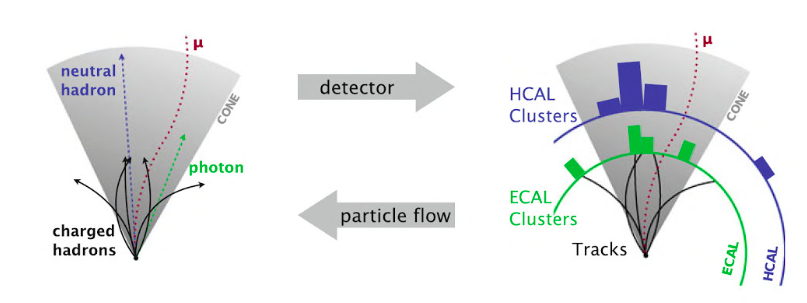
\includegraphics[width=0.75\textwidth]{figures/jets.png}
 	\singlespace
 	\caption{CMS Particle Flow algorithm. The diagram shows how collisions lead to particle decays and final state particles. On the right side of the diagram the tracks and deposits in the CMS detector are shown. The left side shows that PF candidates are derived from detector information and then become input for the PF algorithm that uses them to construct high-level physics objects like electrons, which are then used by analysts to reconstruct the collision event. Reprinted from \cite{CMS-PAS-PFT-09-001}}
 \end{figure}

\section{Jets}

During proton-proton collisions, the confined state of quarks and gluons is broken. This de-confined state of the free partons does not last very long, as it is not allowed by QCD. Shortly after the collision, partons hadronize and a bunch of particles is generated by this process. These particles are usually collimated in a given direction due to the boosted nature of the parton, and thereby producing a jet or spray of particles around it.

\begin{figure}[h]
  	\label{fig:jets2}
 	\centering
 	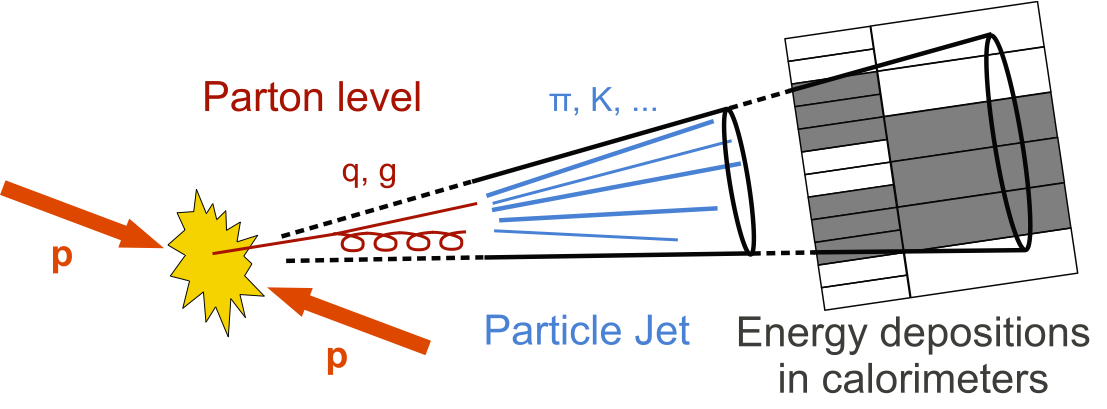
\includegraphics[width=0.75\textwidth]{figures/jetsatcmsand.png}
 	\singlespace
 	\caption{Diagram of proton-proton collision producing a jet}
 \end{figure}

In practice, jets are the result of clustering groups of charged hadrons, photons, and neutral hadrons coming from PF. The energy fraction in jets is divided amongst them with a breakdown of roughly 65$\%$, 25$\%$, and 10$\%$ respectively. This is illustrated in Figure \ref{fig:jme}. For this study, jets were reconstructed from PF candidates clusters using the anti-$k_{T}$ algorithm\cite{Cacciari:2008gp} as defined in the FASTJET package\cite{Cacciari:2011ma}.

\begin{figure}[h]
  	\label{fig:jme}
 	\centering
 	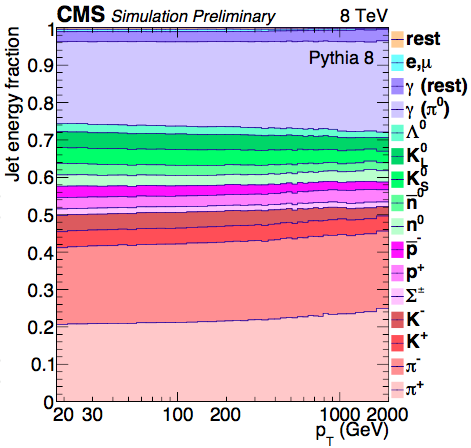
\includegraphics[width=0.75\textwidth]{figures/jme.png}
 	\singlespace
 	\caption{Jet composition}
 \end{figure}

 Jet clustering algorithms work by defining a distance parameter($d_{ij}$) between to PF candidates $i$ and $j$, and the distance between such cluster and the beam, $d_{iB}$. These are defined as

 \begin{align}
 \label{jetclust}
 d_{ij} = min(k_{ti}^{2p},k_{tj}^{2p})\frac{\Delta_{ij}^{2}}{R^{2}}
 d_{iB} &= k_{ti}^{2p}
 \end{align}

where $\Delta_{ij}^{2} = (y_{i}-y_{j})^{2}+(\phi_{i}-\phi_{j})^{2}$, and $k_{ti}$, $y_{i}$, and $\phi_{i}$ are the transverse momentum, rapidity, and azimuth of particle $i$, respectively. R is a user-defined radius parameter, and $p$ is a measure of the relative power of energy vs geometric scales. Particularly, for the anti-$k_{T}$ algorithm, $p=-1$, and Equation \ref{jetclust} reduces to

\begin{equation}
d_{ij} = min(\frac{1}{p_{ti}^{2}},\frac{1}{p_{tj}^{2}})\frac{\Delta_{ij}^{2}}{R^{2}}
\end{equation}

The algorithm loops over all PF candidate objects, calculating $d_{ij}$ for each pair of objects. Once it does this, it selects the two objects with the lowest value of $d_{ij}$ and combines them. This process is repeated until the smallest value of $d_{ij}>d_{iB}$ for all the remaining pairs. 

As a result, the cutoff limit of $1/p_{T}^{2}$ defines a maximum size that the algorithm will look to cluster particles inside. The construction of $d_{ij}$ using the inverse $p_{T}^{2}$ has a result of producing values of $d_{ij}$ that are smaller for objects with a higher $p_{T}$, given equal separation. As a result, softer particles will tend to cluster to higher $p_{T}$ particles long before they would cluster amongst themselves. If no hard particles are present, the jet object will simply cluster soft $p_{T}$ particles in a circle in an $\eta-\phi$ space of radius R.

The clustering of the anti-$k_{T}$ algorithm leads to jets with a large $p_{T}$ being reconstructed as perfect circles, while softer jets can have a more ambiguous shape. Figure \ref{fig:antikt} shows a display of the anti-$k_{T}$ algorithm for a distance parameter R=1. Notice that the green jet around $y=2$ and $\phi=5$ has a circular shape, while it deforms the smaller jet right next to it.

Finally, the anti-$k_{T}$ algorithm is both infrared and collinear safe. Infrared safety means that the jet clustering algorithm is insensitive to the emission of soft, wide angle particles. Under this condition, two jets would not be merge due to one of them producing a high-momentum particle between them. Collinear safety means that if there is a splitting which results in two parallel high-$p_{T}$ particles, a single jet is produced and the jet properties will not be different from a jet where this splitting did not occur. If the algorithm follows these two properties, it is referred to as being IRC safe.

\begin{figure}[h]
  	\label{fig:antikt}
 	\centering
 	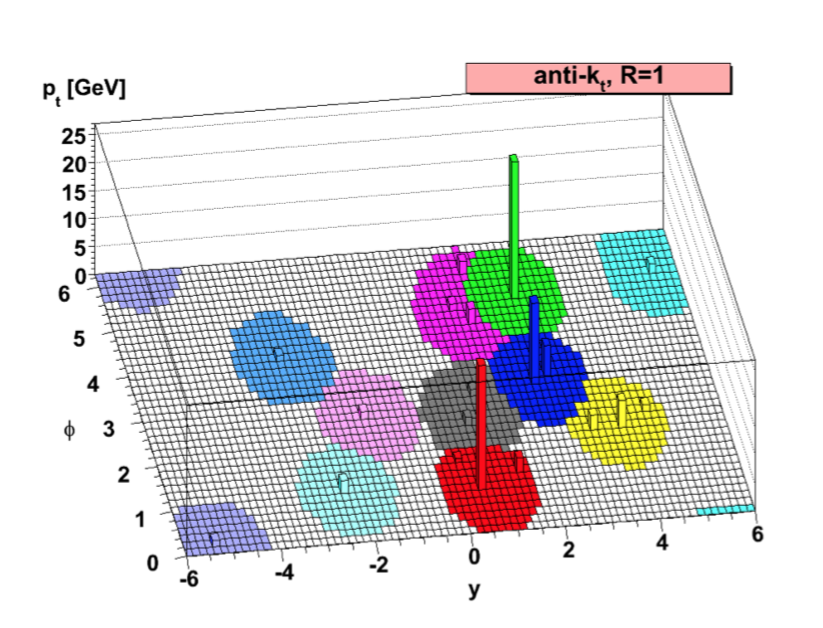
\includegraphics[width=0.75\textwidth]{figures/antikt.png}
 	\singlespace
 	\caption{A sample parton-level event clustered with the anti-$k_{T}$ algorithm. Reprinted from \cite{Cacciari:2008gp}}
 \end{figure}

The use of PF candidates, with their built in tracking information for jet reconstruction provides a jet resolution of 15$\%$ at 10 GeV, 8$\%$ at 100 GeV, and 4$\%$ at 1 TeV\cite{CMS-PAS-PFT-09-001}. 

After the clustering procedure, the momentum and energy of the reconstructed jets still might not be the same as those from the initial parton, whether because of additional pileup energy produced during the same bunch crossing as the primary vertex or detector effects. To correct for this, CMS adopted a factorized approach, where each level of correction targets a specific effect and each correction factor obtained is applied in order. The goal is to make sure each jet has a relative response

\begin{equation}
\mathcal{R}_{rel} = \frac{p_{T}^{reco}}{p_{T}^{ref}} 
\end{equation}

as close as possible to unity. Here $p_{T}^{reco}$ is the reconstructed jet $p_{T}$ and $p_{T}^{ref}$ is the true of reference $p_{T}$ of the jet. 

The process of correcting the jet 4-momentum by means of a scale or weight obtained from matching the reconstructed jet information to that of the reference jet in Monte Carlo is referred to as jet energy correction (JEC).

The first level of correction, commonly referred to as the L1FastJet corrections, starts by removing pileup or electronic noise energy that may have made it into the jet reconstruction. This multiplicative correction will only remove energy from within the jet and will take the form in Equation \ref{pileupeq}, where $\rho$ is the median energy density of the event, $A$ is the jet area, and $f$ is an estimate of the offset inside the jet per unit of jet area \cite{JINST2011,Cacciari2007}.

\begin{equation}
\label{pileupeq}
p_{T}^{L1Corrected} = p_{T}^{uncorrected}\dot(1 - A\frac{f(\eta,\rho,A)}{p_{T}^{uncorrected}})
\end{equation}

The L2Relative correction compensates for the non-linearity in the jet response as a function of $\eta$ while the L3Absolute correction does the same thing as a function of $p_{T}$. All three corrections are applied to both data and simulation. An additional level of correction, called L2L3Residual, is applied to data only in order to correct for the difference in scale between the data and simulation.

A final level of modification to the reconstructed objects is an $\eta$ dependent smearing factor applied to the jet 4-momenta coming from the MC samples. The distribution of jet energies within the MC simulation tends to be more sharply peaked and less broad than the same distribution in data, resulting in a smaller jet energy resolution (JER) than we can realistically measure using the CMS detector. The deterministic "smearing" method recommended by CMS matches the MC jet energy resolution to that in data. 

The reconstructed jet $p_{T}$ is scaled by a correction factor $C_{JER}$ as determined in Equation \ref{eq:C_JER}, where $C_{\eta}$ is a correction factor derived as a function of $\eta$. The multiplicative JER correction factor is then used to modify the jet 4-momentum as in Equation \ref{eq:Jet_JER}.

\begin{equation}
\label{eq:C_JER}
C_{JER}=max\left(0.0,\frac{p_{T}^{GEN}}{p_{T}^{RECO}}+C_{\eta}\cdot\left(1-\frac{p_{T}^{GEN}}{p_{T}^{RECO}}\right)\right)
\end{equation}

\begin{equation}
\label{eq:Jet_JER}
\textbf{X}_{Jet}^{corrected}=C_{JER}{\cdot}\textbf{X}_{Jet}^{RECO}
\end{equation}

A set of quality cuts, collectively called PF jet identification, are applied to the resulting collection of jets to ensure that only real, hard scatter PF jets are used during the analysis\cite{CMS-AN-2010-003}. Several working point are defined at varying levels of efficiency and purity, but this analysis makes use of the tight criteria shown in Table \ref{tab:PFJetID}\cite{PFJetID}.

\begin{table}[htbp]
    \caption{Cut based PF jet identification requirements for the tight working point.}
    \centering
    \begin{tabular}{llll}
        \hline
        \multirow{2}{*}{Cut Variable}               & Cut Value \\\cline{2-2}
                                                    & Tight\\ 
        \hline 
        $\eta$& $|\eta|<$2.7 &2.7$<|\eta|\leq$ 3.0  & $|\eta|>$ 3.0\\
        \hline 
        Neutral Hadron Fraction  & <0.90  & <0.98 & -\\  
        Neutral EM Fraction      & <0.90  & > 0.01 & <0.90\\
        $n_{constituents}$       & >1     & -      & - \\
        Muon fraction            & <0.8   & -      & -\\
        Number of Neutral Particles & - & > 2      & >10\\
        \hline
        and for $|\eta| \leq$ 2.4 in addition apply\\
        \hline
        Charged Hadron Fraction & > 0 \\
        Charged Multiplicity    & > 0 \\
        Charged EM Fraction     & < 0.90\\
        \hline 
    \end{tabular}
    \label{tab:PFJetID}
\end{table}

All cuts on the jet energy fractions are made on the raw jets, before any energy correction is applied. In addition to the PF jet quality cuts, this analysis requires that all jets be within |$\eta$| < 2.6 and to have a $p_{T} > $ 30 GeV. 

\section{b-tagging}
Some jets are produced from a b-quark that after hadronization gets transformed into a B meson that has a large lifetime, and subsequently decay after it has traveled some distance. B-tagging is the identification of jets at some confidence level as having decayed from a B meson.

\begin{figure}[h]
  	\label{fig:antikt}
 	\centering
 	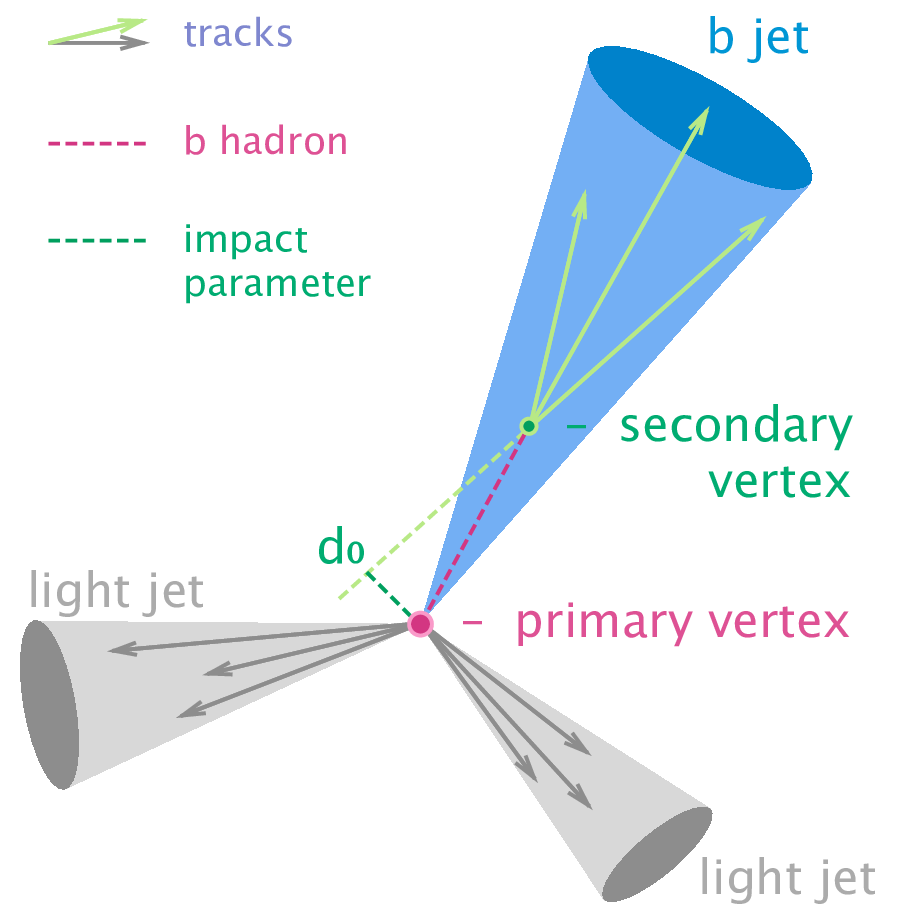
\includegraphics[width=0.75\textwidth]{figures/Btag.png}
 	\singlespace
 	\caption{Diagram showing the common principle of identification of jets initiated by B hadron decays. Reprinted from \cite{wiki:btag}}
 \end{figure}

A variety of b-tagging algorithms has been developed by CMS to select b-quark jets\cite{BTV-12-001} based on variables such as the impact parameters of the charged-particle tracks, the properties of reconstructed decay vertices, and he presence or absence of a lepton, or combinations thereof. These algorithms heavily rely on machine learning tools and are thus natural candidates for advanced tools like deep neural networks. 

A new algorithm, DeepCSV\cite{Sirunyan_2018, PhysRevD.94.112002}, uses a deep neural network. The input is the same set of observables used by the existing CSVv2 b-tagger (Table \ref{tab:csvv2var})\cite{Weiser:927399}, but using more hidden layers, more nodes per layer, and a simultaneous training in all vertex categories and for all jet flavors. Also, the training strategy was adapted and about 50 million jets are used for the training of the deep neural network. The new DeepCSV algorithm outperforms the CSVv2 tagger, with an absolute b-tagging efficiency improvement of about 4$\%$ for a misidentification probability for light flavor jets of 1$\%$. 

\begin{table}[htbp]
    \caption{Input variables used for the CSVv2 algorithm.}
    \centering
    \begin{tabular}{l}
        \hline
        %\multirow{2}{*}{Cut Variable}               & Cut Value \\\cline{2-2}
        Input variable                                            \\ 
        \hline 
        Secondary vertex 2D flight distance significance\\
        Number of secondary vertices\\
        Track $\eta_{rel}$\\
        Corrected secondary vertex mass\\
        Number of track from secondary vertex\\
        Secondary vertex enegry ratio\\
        $\Delta R (Secondary vertex, jet)$ \\
        3D interaction point significance of the first four tracks\\
        Track $p_{T,rel}$\\
        $\Delta R (track, jet)$ \\
        Track $p_{T,rel}$ ratio\\
        Track distance\\
        Track decay length\\
        Summed tracks $E_{T}$ ratio\\
        $\Delta R$(summed tracks, jet)\\
        First track 2D interaction point significance above c threshold\\
        Number of selected tracks\\
        Jet $p_{T}$\\
        Jet $\eta$\\
        \hline 
    \end{tabular}
    \label{tab:csvv2var}
\end{table}

This algorithm uses the reconstructed tracks and secondary vertices found by using the \textit{inclusive vertex finding} (IVF) algorithm \cite{ADAM2007781}. The same input variables used for the CSVv2 tagger are used, with the difference that the track-based variables use up to six tracks in the training of the DeepCSV. Jets are randomly selected in such a way that similar jet $p_{T}$ and $\eta$ distributions are obtained for all jet flavors. These distributions are also used as input variables in the training to take into account the correlation between the jet kinematics and the other variables. The distribution of all input variables is preprocessed to center the mean of each distribution around zero and to obtain a root-mean-square value of unity. All of the variables are presented to the multi-variable analysis (MVA) in the same way because of the preprocessing.

The training is performed using jets with $p_{T}$ between 20 GeV and 1 TeV, and within the tracker acceptance. The relative ratio of jets of each flavor is set to 2:1:4 for b:c:udsg jets. a mixture of $t\bar{t}$ and multi-jet events is used to reduce the possible dependency of the training on the heavy-flavor quark production process.

The training of the deep neural network is performed using the KERAS\cite{chollet2015keras} deep learning library, interfaced with the TENSORFLOW\cite{tensorflow2015-whitepaper} library that is used for low-level operations such as convolutions. The neural network uses four hidden layers that are fully connected, each with 100 nodes. For the nodes in the last layer, a normalized exponential function is used for the activation to be able to interpret the output value as a probability for a certain jet flavor category, $P(f)$. The output layer contains five nodes corresponding to five jet flavor categories used in the training. These categories are defined according to whether the jet contains exactly one b hadron, at least two b hadrons, exactly one c hadron and no b hadrons, at least two c hadrons and no b hadrons, or none of the aforementioned categories. Each of these categories is completely independent of the others, and the reasoning behind the chosen categorization has to do with the ability to provide analysis to identify jets containing two b or c hadrons. 

The tagger can categorize individual jets in so-called "Tight" (DeepCSVT), "Medium"(DeepCSVM), and "Loose"(DeepCSVL) categories or working points. These working points correspond to 0.1, 1, and 10 $\%$ misidentification rates, respectively.

Figure \ref{fig:deepcsv} shows the b-jet efficiency as a function of the jet $p_{T}$ for the DeepCSV algorithm at different working points. These efficiencies are obtained on simulated $t\bar{t}$ events using jets within tracker acceptance with $p_{T}$ > 30 GeV.

\begin{figure}[h]
  	\label{fig:deepcsv}
 	\centering
 	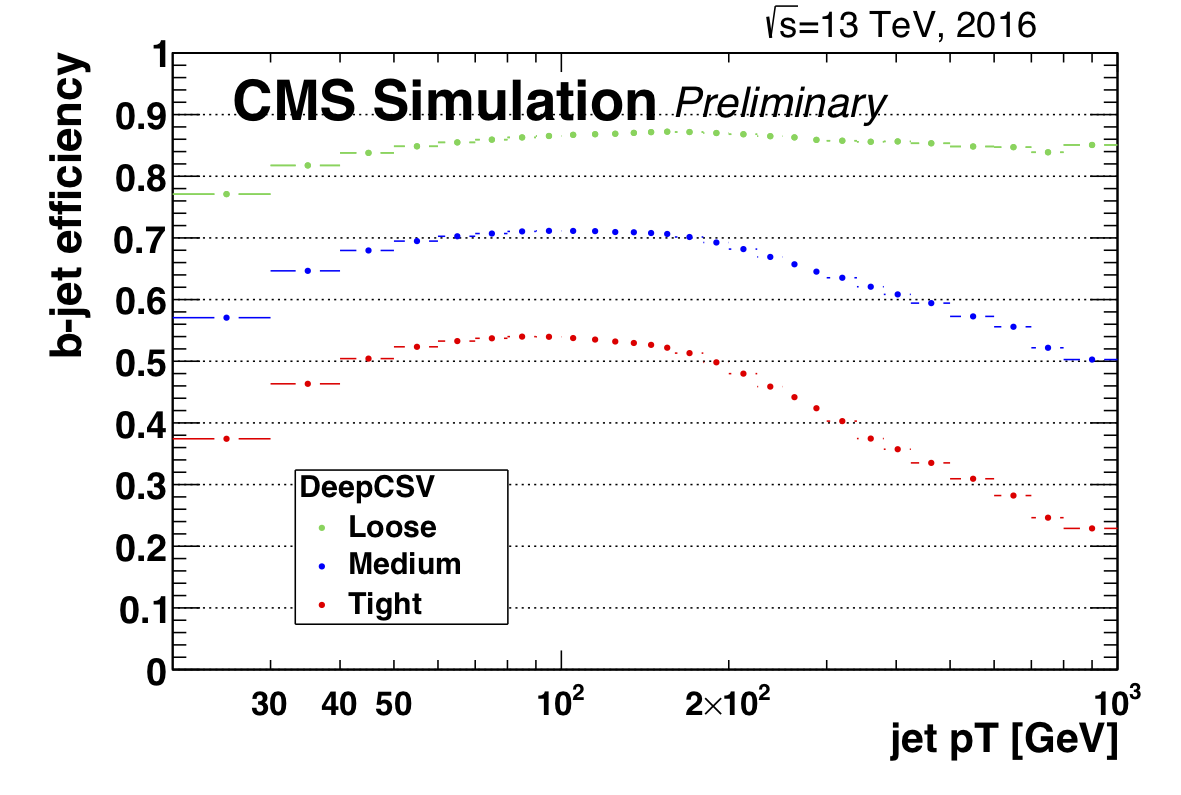
\includegraphics[width=0.75\textwidth]{figures/effvspt_b_deep.png}
 	\singlespace
 	\caption{b-jet efficiency as a function of jet $p_{T}$ for the DeepCSV algorithm. \cite{Sirunyan_2018}}
 \end{figure}

\section{Event Generation}
Searching for new physics can basically be reduced to a search for deviations from the SM. For this reason, extremely accurate signal and SM background predictions are required. For a given analysis, these predictions take the form of samples of events representing various physics scenarios, as they would be seen in the CMS detector. Monte Carlo (MC) event generators are used to simulate proton-proton collisions resulting in a variety of final states. The passage of these final states through the CMS detector is then simulated, and the resulting detector level data is analyzed. The reconstruction algorithms described in the previous section are then run on the simulated data, allowing for a direct comparison with real data.

\subsection{Event Generators}
Event generators are software packages which take as input a desired initial state and simulate all possible outcomes, or a selected subset of outcomes, from an interaction between the specified initial state particles. Bare partons produced in the hard scattering undergo gluon radiation or splitting, and subsequently undergo hadronization to form colorless hadrons. Unstable particle produced in the hard interaction or parton shower are made to decay to stable particles according to their known, or imposed, branching fractions and lifetimes.

During the event generation process, partons which take part in hard scattering interactions with large momentum transfer can be considered free due to asymptotic freedom. The large energy scale involved allows treatment of the interaction using perturbative methods. Under these assumptions, the proton-proton cross section at the LHC for a given $N$ particle final state is given by

\begin{equation}
\sigma_{N} = \sum_{a,b}\int_{0}^{1}dx_{1}\int_{0}^{1}dx_{2}f_{a}(x_{1},\mu^{2})f_{b}(x_{2},\mu^{2})\hat{\sigma}_{N}^{ab}
\end{equation}

where the sum is over all parton species $a$ and $b$ within protons 1 and 2. $f_{i}(x_{j},\mu^{2})$ is the probability (calculated at renormalization scale $\mu^{2}$) of finding parton species $i$ carrying a momentum fraction $x_{j}$ of the parent proton $j$, and $\hat{\sigma}_{N}^{ab}$ is the partonic cross section for initial state $a+b$. The function $f_{i}(x_{j},\mu^{2})$ is referred to as a parton distribution function (PDF). The main task involved in simulation of the hard interaction is the evaluation of this integral. The partonic cross section is itself given by

\begin{equation}
\begin{split}\label{eq:event_generation_partonic_cross_section}
\hat{\sigma}_{N}^{ab}=\int_{cuts}d\hat{\sigma}_{N}^{ab}={}&\frac{\left(2\pi\right)^{4}S}{4\sqrt{\left(p_{1}{\cdot}p_{2}\right)^{2}-m_{1}^{2}m_{2}^{2}}}\times \\ &\int_{cuts} \left[\prod_{i=1}^{N}\frac{d^{3}q_{i}}{\left(2\pi\right)^{3}2E_{i}}\right]\delta^{4}\left(p_{1}+p_{2}-\sum_{i}^{N}q_{i}\right)|\mathcal{M}_{p_{1}p_{2}\rightarrow\{\vec{q}\}}^{ab}|^{2}
\end{split}
\end{equation}

where $p_{i}$ are the incoming particle four-momenta, $q_{i}(E_{i})$ are the outgoing particle four-momenta, $S$ is a product of factors $1/j!$ for each set of $j$ identical particles in the final state, and $\mathcal{M}_{p_{1}p_{2}\rightarrow\{\vec{q}\}}^{ab}$ is the parton level matrix element (ME) for the process. The event generator must build and evaluate all Feynman diagrams associated with the given process to determine the parton level ME, or these must be hard-coded by the package authors. 

The number of diagrams is directly proportional to the final state multiplicity and therefore becomes a complex problem very quickly. Next-to-leading-order (NLO) generators have recently been developed which include loop diagrams. This inclusion complicates the matter enormously as divergences arise in real and virtual contributions which must cancel. 

Once the MEs have been evaluated, the evaluation of the multidimensional phase space integration required for the random sampling is performed using MC techniques. The spectator partons which did not take part in the initial hard interaction can undergo semi-hard interactions with each other, which is referred to as the underlying event (UE). Because these spectator interactions are typically soft, they are not calculable by perturbative methods and empirical models are used to describe them.

Bare partons may be produced as a result of the hard interaction. These partons are perturbatively evolved from the scale of the hard interaction through successive branchings down to a lower energy scale at which they combine to form colorless hadrons, the hadronization scale. These successive branchings are the origin of hadronic jets, whereby individual partons lead to a cascade of partons moving in the general direction of the original parton and sharing its momentum. The probability for a parton to branch into two partons as it evolves from scale $t$ to $t'<t$ and the kinematics of such a branching can ce calculated form first principles, accurate to fixed order in the strong coupling; the results of which are known as the DGLAP evolution equations. Thus, the partons are recursively evolved down to the hadronization scale through successive branchings. Care must be taken to avoid double counting of regions in phase-space. After showering of an N-1 particle final state, an additional hard parton can be radiated, thus producing overlap with an $N$ particle interaction hard state. The colored proton remnants which did not take part in the hard interaction can produce showers as well. 

At the hadronization scale, the showering ceases and the colored partons group to form colorless hadrons. This regime is not amenable to perturbative calculations, and no first-principle theory is viable. Various phenomenological methods have been developed to model hadronization, including the \textit{Lund-string-model} and the \textit{cluster hadronization model}. In the Lund model, color string attach to a pair of quarks, and as these strings stretch, energy is built up in the electromagnetic field until vacuum excitation of a quark-antiquark pair becomes possible. Ultimately, color connected pairs of quarks form hadrons. 

The cluster hadronization model assumes a local parton-hadron duality, this hadronic quantum numbers result from the quantum numbers of local partons with minimal disruption needed to produce colorless hadrons. Regardless of the hadronization model choice, the produced hadrons are often unstable, and are then decayed to stable hadrons.

\subsubsection{Pythia}

PYTHIA is a general purpose, tree level partonic ME generator capable of performing parton showering, hadronization, and UE simulation. A variety of $2\rightarrow1,2,3$ processes are included. Full spin correlations are included in the decays of unstable resonances. Shower evolution proceeds in terms of decreasing time-like virtuality, and imposes angular ordering by veto. Shower evolution is accurate to the LL level. The Lund string model is used for hadronization. UE interactions are described perturbatively as multiple nearly-independent $2\rightarrow 2$ scatterings. PYTHIA 8 is used in this analysis to simulate signal samples with $xqcut=30$ and $qcut=60$.

\subsubsection{MADGRAPH}

MADGRAPH is another generator that is used in this analysis for simulating hard parton emission (ie. ISR and FSR), but must be interfaced with PYTHIA for showering and collinear radiation.

\subsection{Detector Simulation}

The next step in the simulation of events chain is the simulation of how particles will interact with the detector and its constituent materials or how the readout electronics will behave. To simulate the response of the CMS detector, the generators are interfaced with a sophisticated detector simulation based on the GEANT4 software package, which takes into account the exact detector geometry as well as all materials used.

The alignment, calibration, and other conditions which may change over time are periodically checked and stored in a database. These conditions are used for both offline simulation and reconstruction as well as for online activities. A snapshot of the conditions at some point in time is called a global tag. For reference, this analysis uses the $80X\_dataRun2\_2016LegacyRepro\_v4$ and $80X\_mcRun2\_asymptotic\_2016\_TrancheIV\_v8$ global tags for data and simulation, respectively. 

The final state particles from the event generator are sent to the detector simulation, which tracks the particles as they move through the detector depositing energy into what are called simulated hits. While the models of electromagnetic interactions are extremely precise, the hadronic interactions have a greater uncertainty associated with them. The simulation goes through the data acquisition process, event simulating the responses of the photodetectors and readout electronics. The resulting information is then analyzed by the same reconstruction process that the real data goes through and is stored using the ROOT software library. 


%The next line is the format for inserting new sections.
%Replace the name "newsection"  with the name of your
%new section file.
%\include{data/newsection}

%fix spacing in bibliography, if any...
%%%%%%%%%%%%%%%%%%%%%%%%%%%%%%%%%%%%%%%%%%%%%%%%%%%%%%%%%%%%%
\let\oldbibitem\bibitem
\renewcommand{\bibitem}{\setlength{\itemsep}{0pt}\oldbibitem}
%%%%%%%%%%%%%%%%%%%%%%%%%%%%%%%%%%%%%%%%%%%%%%%%%%%%%%%%%%%%%%%
%The bibliography style declared is the IEEE format. If
%you require a different style, see the document
%bibstyles.pdf included in this package. This file,
%hosted by the University of Vienna, shows several
%bibliography styles and examples of in-text citation
%and a references page.
\bibliographystyle{ieeetr}

\phantomsection
\addcontentsline{toc}{chapter}{REFERENCES}

\renewcommand{\bibname}{{\normalsize\rm REFERENCES}}

%This file is a .bib database that contains the sources.
%This removes the dependency on the previous file
%bibliography.tex.
\bibliography{data/myReference}




%This next line includes appendices. The file
%appendix.tex contains commands pointing to
%the appendix files; be sure to change these
%pointers if you end up changing the filenames.
%Leave this commented if you will not need
%appendix material.
%%%%%%%%%%%%%%%%%%%%%%%%%%%%%%%%%%%%%%%%%%%%%%%%%%%%
%
%  New template code for TAMU Theses and Dissertations starting Fall 2016.  
%
%
%  Author: Sean Zachary Roberson
%  Version 3.17.09
%  Last Updated: 9/21/2017
%
%%%%%%%%%%%%%%%%%%%%%%%%%%%%%%%%%%%%%%%%%%%%%%%%%%%

\begin{appendices}
\titleformat{\chapter}{\centering\normalsize}{APPENDIX \thechapter}{0em}{\vskip .5\baselineskip\centering}
\renewcommand{\appendixname}{APPENDIX}

%%%%%%%%%%%%%%%%%%%%%%%%%%%%%%%%%%%%%%%%%%%%%%%%%%%
%
%  New template code for TAMU Theses and Dissertations starting Fall 2016.
%
%
%  Author: Sean Zachary Roberson 
%	 Version 3.16.09
%  Last updated 9/12/2016
%
%%%%%%%%%%%%%%%%%%%%%%%%%%%%%%%%%%%%%%%%%%%%%%%%%%%

%%%%%%%%%%%%%%%%%%%%%%%%%%%%%%%%%%%%%%%%%%%%%%%%%%%%%%%%%%%%%%%%%%%%%%
%%                           APPENDIX A 
%%%%%%%%%%%%%%%%%%%%%%%%%%%%%%%%%%%%%%%%%%%%%%%%%%%%%%%%%%%%%%%%%%%%%

\phantomsection

\chapter{\uppercase{First Appendix}}

Text for the Appendix follows.

\begin{figure}[h]
\centering
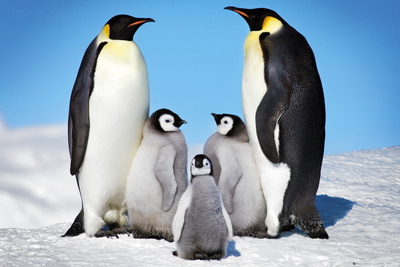
\includegraphics[scale=.50]{figures/Penguins.jpg}
\caption{TAMU figure}
\label{fig:tamu-fig5}
\end{figure}

%%%%%%%%%%%%%%%%%%%%%%%%%%%%%%%%%%%%%%%%%%%%%%%%%%%
%
%  New template code for TAMU Theses and Dissertations starting Fall 2016.
%
%
%  Author: Sean Zachary Roberson 
%	 Version 3.16.09 
%  Last updated 9/12/2016
%
%%%%%%%%%%%%%%%%%%%%%%%%%%%%%%%%%%%%%%%%%%%%%%%%%%%

%%%%%%%%%%%%%%%%%%%%%%%%%%%%%%%%%%%%%%%%%%%%%%%%%%%%%%%%%%%%%%%%%%%%%%
%%                           APPENDIX B
%%%%%%%%%%%%%%%%%%%%%%%%%%%%%%%%%%%%%%%%%%%%%%%%%%%%%%%%%%%%%%%%%%%%%

\chapter{\uppercase {A Second Appendix Whose Title Is Much Longer Than The First}}

Text for the Appendix follows.

\begin{figure}[h]
\centering
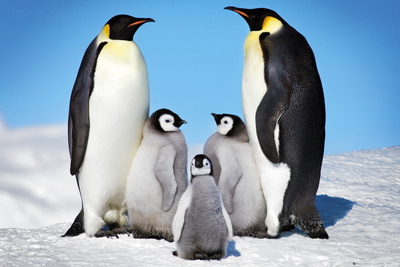
\includegraphics[scale=.50]{figures/Penguins.jpg}
\caption{Another TAMU figure.}
\label{fig:tamu-fig6}
\end{figure}

\section{Appendix Section}

\section{Second Appendix Section}


\pagebreak{}

\end{appendices}


\end{document}
